% Requires in the preamble:
% \usepackage{amsmath,amssymb}
% \usepackage{tikz,pgfplots}
% \pgfplotsset{compat=1.18}

\chapter{Parametric Curves, Polar Coordinates, and Conics}
\label{chap:parametric-polar-conics}

Differential equations taught us to let time drive a function.  A solution might be
written as

\[
t\longmapsto y(t),
\]

where one input \(t\) produces one output \(y\).

But some curves resist being written as

\[
y=f(x).
\]

A circle fails the vertical line test.  A loop may pass above the same \(x\)-value more
than once.  A point on a wheel can rise, fall, and return to the same horizontal
position.

The curve is not the problem.  The notation is the problem.

Instead of forcing one coordinate to depend on the other, we let both coordinates
depend on a parameter:

\[
x=x(t),
\qquad
y=y(t).
\]

A moving point draws the curve.

\section{Parametric curves}
\label{sec:parametric-curves}

A graph \(y=f(x)\) is one way to describe a curve.  A parametric description is another.
It is often closer to the way the curve is actually produced.

A particle has a horizontal position and a vertical position.  A wheel point has an
\(x\)-coordinate and a \(y\)-coordinate.  A planet has two coordinates in a plane.  In
each case, time does not have to appear on the final picture, but it may be the easiest
way to draw the picture.

\[
\boxed{
\text{A parametric curve is a curve traced by a moving point.}
}
\]

\subsection{A curve as a moving point}
\label{subsec:curve-as-moving-point}

Imagine a point moving around the unit circle.  At time \(t\), put

\[
x(t)=\cos t,
\qquad
y(t)=\sin t.
\]

Then the point has position

\[
P(t)=(x(t),y(t))=(\cos t,\sin t).
\]

When \(t=0\),

\[
P(0)=(1,0).
\]

When \(t=\pi/2\),

\[
P(\pi/2)=(0,1).
\]

When \(t=\pi\),

\[
P(\pi)=(-1,0).
\]

When \(t=3\pi/2\),

\[
P(3\pi/2)=(0,-1).
\]

As \(t\) increases from \(0\) to \(2\pi\), the point travels once around the circle in the
counterclockwise direction.

\begin{figure}[h]
\centering
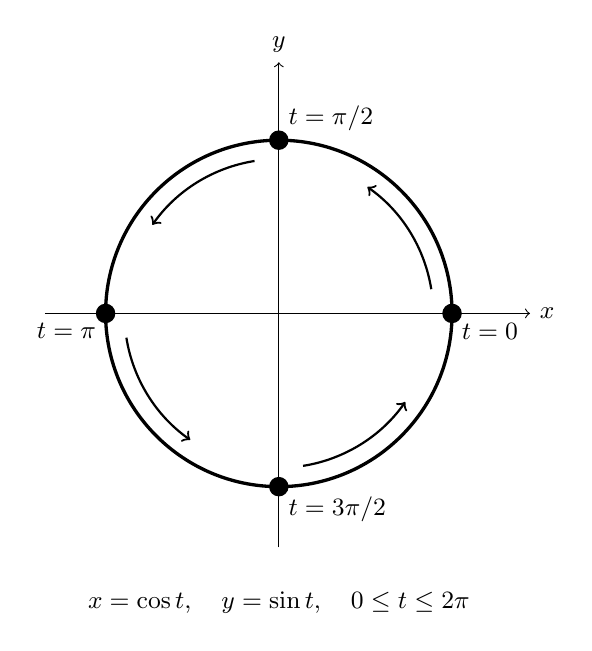
\begin{tikzpicture}[scale=2.2, every node/.style={font=\small}]
  % axes
  \draw[->] (-1.35,0) -- (1.45,0) node[right] {\(x\)};
  \draw[->] (0,-1.35) -- (0,1.45) node[above] {\(y\)};

  % circle
  \draw[very thick] (0,0) circle (1);

  % arrows along circle
  \draw[->, thick] (0.88,0.14) arc (9:55:0.89);
  \draw[->, thick] (-0.14,0.88) arc (99:145:0.89);
  \draw[->, thick] (-0.88,-0.14) arc (189:235:0.89);
  \draw[->, thick] (0.14,-0.88) arc (279:325:0.89);

  % points
  \fill (1,0) circle (1.6pt);
  \fill (0,1) circle (1.6pt);
  \fill (-1,0) circle (1.6pt);
  \fill (0,-1) circle (1.6pt);

  \node[below right] at (1,0) {\(t=0\)};
  \node[above right] at (0,1) {\(t=\pi/2\)};
  \node[below left] at (-1,0) {\(t=\pi\)};
  \node[below right] at (0,-1) {\(t=3\pi/2\)};

  \node at (0,-1.67) {\(x=\cos t,\quad y=\sin t,\quad 0\le t\le 2\pi\)};
\end{tikzpicture}
\caption{The parameter \(t\) tells how the point moves around the circle.}
\label{fig:parametric-unit-circle}
\end{figure}

The curve itself is the circle.  The parametrization tells more: it tells where the point is
at each time, the direction of travel, and how fast the point moves.

This extra information is often useful.  A road map shows the road.  A schedule tells
how the traveler moves along it.  A parametric curve contains both.

\begin{quote}
\textbf{Parametrization of a plane curve.}
A \emph{parametrization} of a plane curve is a pair of functions

\[
x=x(t),
\qquad
y=y(t),
\]

defined for \(t\) in an interval \(I\).  The moving point

\[
P(t)=(x(t),y(t))
\]

traces the curve as \(t\) runs through \(I\).

The variable \(t\) is called a \emph{parameter}.  It is often time, but it does not have
to be.
\end{quote}

The interval for \(t\) is part of the description.  For example,

\[
x=\cos t,
\qquad
y=\sin t,
\qquad
0\le t\le 2\pi
\]

traces the full unit circle once.

But

\[
x=\cos t,
\qquad
y=\sin t,
\qquad
0\le t\le \pi
\]

traces only the upper semicircle.

The formulas alone do not tell the whole story.  The parameter interval matters.

\subsection{Eliminating the parameter when possible}
\label{subsec:eliminating-parameter}

Sometimes a parametric curve can be translated into an ordinary Cartesian equation by
removing the parameter.

For the circle example,

\[
x=\cos t,
\qquad
y=\sin t.
\]

Since

\[
\cos^2 t+\sin^2 t=1,
\]

we get

\[
x^2+y^2=1.
\]

That is the Cartesian equation of the unit circle.

This equation tells the geometric shape.  It does not tell the direction of motion or the
speed.  Those belong to the parametrization.

\paragraph{Example: a line.}
Let

\[
x=1+3t,
\qquad
y=-2+t,
\qquad
0\le t\le 2.
\]

The point starts at

\[
(x(0),y(0))=(1,-2)
\]

and ends at

\[
(x(2),y(2))=(7,0).
\]

To eliminate \(t\), solve the first equation:

\[
t=\frac{x-1}{3}.
\]

Substitute into \(y=-2+t\):

\[
y=-2+\frac{x-1}{3}.
\]

So

\[
y=\frac13x-\frac73.
\]

The parametrization traces the line segment on this line from \((1,-2)\) to \((7,0)\).

\begin{figure}[h]
\centering
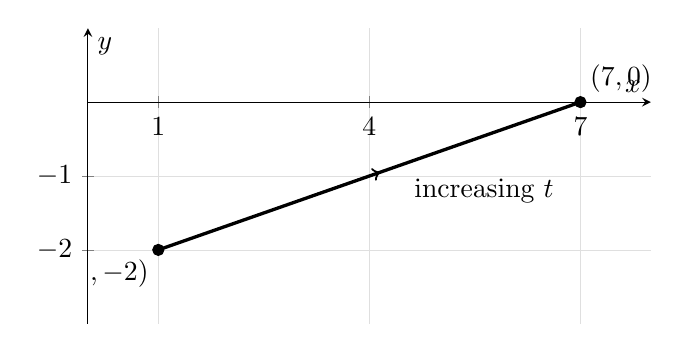
\begin{tikzpicture}
\begin{axis}[
    width=0.72\textwidth,
    height=0.44\textwidth,
    xmin=0, xmax=8,
    ymin=-3, ymax=1,
    axis lines=middle,
    xlabel={\(x\)},
    ylabel={\(y\)},
    xtick={1,4,7},
    ytick={-2,-1,0},
    grid=both,
    grid style={line width=.1pt, draw=gray!25},
]
\addplot[very thick, domain=1:7, samples=2] {(x-1)/3 - 2};
\addplot[only marks, mark=*] coordinates {(1,-2) (7,0)};
\draw[->, thick] (axis cs:3.15,-1.28) -- (axis cs:4.15,-0.95);
\node[anchor=north east] at (axis cs:1,-2) {\((1,-2)\)};
\node[anchor=south west] at (axis cs:7,0) {\((7,0)\)};
\node[anchor=west] at (axis cs:4.5,-1.2) {increasing \(t\)};
\end{axis}
\end{tikzpicture}
\caption{The equations \(x=1+3t,\;y=-2+t\) trace a line segment with a direction.}
\label{fig:parametric-line-segment}
\end{figure}

The Cartesian equation gives the infinite line.  The parameter interval gives the segment.

\paragraph{Example: a sideways parabola.}
Let

\[
x=t^2-1,
\qquad
y=t,
\qquad
-2\le t\le 2.
\]

Since \(y=t\), we can substitute directly:

\[
x=y^2-1.
\]

This is a parabola opening to the right.  It is not the graph of a single function
\(y=f(x)\), because most \(x\)-values to the right of \(-1\) have two \(y\)-values.

The parametric form has no trouble with this.  It gives exactly one point for each
value of \(t\):

\[
P(t)=(t^2-1,t).
\]

As \(t\) increases from \(-2\) to \(2\), the point moves down the lower branch to the
vertex \((-1,0)\), then up the upper branch.

\begin{figure}[h]
\centering
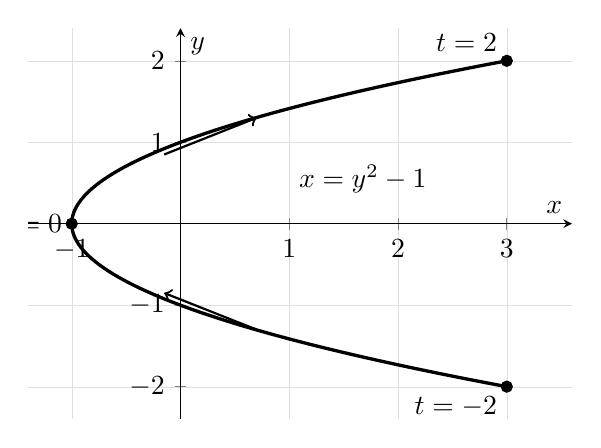
\begin{tikzpicture}
\begin{axis}[
    width=0.70\textwidth,
    height=0.54\textwidth,
    xmin=-1.4, xmax=3.6,
    ymin=-2.4, ymax=2.4,
    axis lines=middle,
    xlabel={\(x\)},
    ylabel={\(y\)},
    xtick={-1,0,1,2,3},
    ytick={-2,-1,0,1,2},
    grid=both,
    grid style={line width=.1pt, draw=gray!25},
]
\addplot[very thick, domain=-2:2, samples=150] ({x^2-1},{x});
\addplot[only marks, mark=*] coordinates {(3,-2) (-1,0) (3,2)};
\draw[->, thick] (axis cs:0.7,-1.3) -- (axis cs:-0.15,-0.85);
\draw[->, thick] (axis cs:-0.15,0.85) -- (axis cs:0.7,1.3);
\node[anchor=north east] at (axis cs:3,-2) {\(t=-2\)};
\node[anchor=east] at (axis cs:-1,0) {\(t=0\)};
\node[anchor=south east] at (axis cs:3,2) {\(t=2\)};
\node[anchor=west] at (axis cs:1.0,0.55) {\(x=y^2-1\)};
\end{axis}
\end{tikzpicture}
\caption{The sideways parabola is easy to trace parametrically: \(x=t^2-1,\;y=t\).}
\label{fig:sideways-parabola-parametric}
\end{figure}

This example shows why parametrization is useful.  The curve is simple, but it is not
a graph \(y=f(x)\).  A moving point can trace it naturally.

\subsection{What elimination forgets}
\label{subsec:what-elimination-forgets}

Eliminating the parameter can be helpful, but it forgets information.

Consider the three parametrizations

\[
x=\cos t,\qquad y=\sin t,\qquad 0\le t\le 2\pi,
\]

\[
x=\cos(2t),\qquad y=\sin(2t),\qquad 0\le t\le 2\pi,
\]

and

\[
x=\cos(-t),\qquad y=\sin(-t),\qquad 0\le t\le 2\pi.
\]

All three satisfy

\[
x^2+y^2=1.
\]

So elimination gives the same Cartesian equation.

But the motions are different.

\begin{center}
\begin{tabular}{c|c|c}
\textbf{parametrization} & \textbf{what it traces} & \textbf{orientation} \\ \hline
\((\cos t,\sin t)\) & unit circle once & counterclockwise \\[3pt]
\((\cos 2t,\sin 2t)\) & unit circle twice & counterclockwise \\[3pt]
\((\cos(-t),\sin(-t))\) & unit circle once & clockwise
\end{tabular}
\end{center}

The same equation

\[
x^2+y^2=1
\]

does not remember how the circle was traced.

\begin{quote}
\textbf{Warning.}
A Cartesian equation describes the set of points on the curve.  A parametrization also
describes the motion along the curve.

When you eliminate the parameter, you may lose:

\[
\text{orientation},\qquad
\text{speed},\qquad
\text{starting point},\qquad
\text{ending point},\qquad
\text{repeated tracing}.
\]
\end{quote}

There is another warning.  Eliminating the parameter can accidentally enlarge the
curve if the parameter interval is ignored.

\paragraph{Example: keep the domain.}
Let

\[
x=t^2,
\qquad
y=t^4,
\qquad
-1\le t\le 1.
\]

Since

\[
y=(t^2)^2,
\]

we get

\[
y=x^2.
\]

But \(x=t^2\), so

\[
0\le x\le 1.
\]

The curve is not the whole parabola \(y=x^2\).  It is only the part from

\[
(0,0)
\]

to

\[
(1,1),
\]

and it is traced twice: once as \(t\) runs from \(-1\) to \(0\), and once as \(t\) runs
from \(0\) to \(1\).

The parameter interval is not decoration.  It is part of the curve's behavior.

\subsection{Different parametrizations of the same curve}
\label{subsec:different-parametrizations-same-curve}

A single geometric curve can have many parametrizations.  This is not a nuisance.  It is
a choice of schedule.

The line segment from \(A=(1,2)\) to \(B=(5,4)\) can be described by

\[
x=1+4t,
\qquad
y=2+2t,
\qquad
0\le t\le 1.
\]

At \(t=0\), the point is \(A\).  At \(t=1\), the point is \(B\).

The same segment can also be described by

\[
x=1+4s^2,
\qquad
y=2+2s^2,
\qquad
0\le s\le 1.
\]

This still starts at \(A\) and ends at \(B\), and it traces the same geometric segment.
But it does not move along the segment at the same rate.

For the first parametrization,

\[
\frac{dx}{dt}=4,
\qquad
\frac{dy}{dt}=2.
\]

The components of motion are constant.

For the second parametrization,

\[
\frac{dx}{ds}=8s,
\qquad
\frac{dy}{ds}=4s.
\]

At \(s=0\), both derivatives are \(0\).  The point starts from rest, then speeds up.

The road is the same.  The trip is different.

\paragraph{A reverse parametrization.}
The segment from \(A=(1,2)\) to \(B=(5,4)\) can also be traced backward:

\[
x=5-4t,
\qquad
y=4-2t,
\qquad
0\le t\le 1.
\]

Now the starting point is \(B\), and the ending point is \(A\).

\begin{quote}
\textbf{Parametrization as schedule.}
A geometric curve tells where the point can be.

A parametrization tells where the point is, in what order, and at what rate.
\end{quote}

This distinction will matter when we compute slopes, lengths, and areas.  The geometry
may be unchanged, but the parameter controls the calculations.

\subsection{Orientation and speed along a curve}
\label{subsec:orientation-speed-along-curve}

When \(t\) is time, the derivatives

\[
\frac{dx}{dt}
\qquad\text{and}\qquad
\frac{dy}{dt}
\]

measure horizontal and vertical velocity.

The speed along the curve is the length of the velocity components:

\[
\boxed{
\text{speed}
=
\sqrt{\left(\frac{dx}{dt}\right)^2+\left(\frac{dy}{dt}\right)^2}.
}
\]

This is the Pythagorean theorem applied to a very small motion.

If during a short time \(\Delta t\),

\[
\Delta x\approx x'(t)\Delta t,
\qquad
\Delta y\approx y'(t)\Delta t,
\]

then the small distance traveled is approximately

\[
\sqrt{(\Delta x)^2+(\Delta y)^2}
\approx
\sqrt{\bigl(x'(t)\Delta t\bigr)^2+\bigl(y'(t)\Delta t\bigr)^2}.
\]

So

\[
\Delta s
\approx
\sqrt{(x'(t))^2+(y'(t))^2}\,\Delta t.
\]

That is why the square root formula is the speed.

\paragraph{Example: speed on the unit circle.}
For

\[
x=\cos t,
\qquad
y=\sin t,
\]

we have

\[
\frac{dx}{dt}=-\sin t,
\qquad
\frac{dy}{dt}=\cos t.
\]

So the speed is

\[
\sqrt{(-\sin t)^2+(\cos t)^2}
=
\sqrt{\sin^2 t+\cos^2 t}
=
1.
\]

The point moves around the unit circle with constant speed \(1\).

For

\[
x=\cos(2t),
\qquad
y=\sin(2t),
\]

we have

\[
\frac{dx}{dt}=-2\sin(2t),
\qquad
\frac{dy}{dt}=2\cos(2t).
\]

The speed is

\[
\sqrt{4\sin^2(2t)+4\cos^2(2t)}
=
2.
\]

The second point moves twice as fast.  On \(0\le t\le2\pi\), it also traces the circle
twice.

\paragraph{Example: a point that pauses.}
Let

\[
x=t^3,
\qquad
y=0.
\]

The curve is the \(x\)-axis.  The point moves along it, passing through the origin at
\(t=0\).  Its speed is

\[
\sqrt{(3t^2)^2+0^2}=3t^2.
\]

At \(t=0\), the speed is \(0\).  The point momentarily stops, then continues moving to
the right.

A zero speed does not always mean the curve ends.  It may only mean the chosen
schedule has a pause.

The next section asks how to do calculus on such curves.  A tangent slope is no longer
found from \(y=f(x)\).  Instead, both \(x\) and \(y\) are changing, and the slope must be
built from their rates.

\section{Calculus with parametric curves}
\label{sec:calculus-parametric-curves}

A parametric curve gives two functions:

\[
x=x(t),
\qquad
y=y(t).
\]

The graph is drawn in the \(xy\)-plane, but the motion is controlled by \(t\).

So a slope question must be translated.

\[
\text{How fast does \(y\) change with respect to \(x\)?}
\]

The parameter tells us two easier facts:

\[
\text{how fast \(y\) changes with respect to \(t\),}
\]

and

\[
\text{how fast \(x\) changes with respect to \(t\).}
\]

The slope \(\dfrac{dy}{dx}\) is the ratio of those two rates.

\subsection{\texorpdfstring{Slope \(dy/dx\) from \(dx/dt\) and \(dy/dt\)}{Slope dy/dx from dx/dt and dy/dt}}
\label{subsec:parametric-slope-formula}

Return to the sideways parabola

\[
x=t^2-1,
\qquad
y=t.
\]

At \(t=1\), the point is

\[
(x,y)=(0,1).
\]

The coordinate rates are

\[
\frac{dx}{dt}=2t,
\qquad
\frac{dy}{dt}=1.
\]

At \(t=1\),

\[
\frac{dx}{dt}=2,
\qquad
\frac{dy}{dt}=1.
\]

This means that near \(t=1\), a small increase in time produces about twice as much
horizontal change as vertical change.  The tangent slope should be

\[
\frac{\text{vertical change}}{\text{horizontal change}}
=
\frac{1}{2}.
\]

That is exactly the ratio

\[
\frac{dy/dt}{dx/dt}.
\]

\begin{quote}
\textbf{Parametric slope formula.}
Suppose \(x(t)\) and \(y(t)\) are differentiable near \(t=t_0\), and

\[
\frac{dx}{dt}(t_0)\neq0.
\]

Then the slope of the parametric curve at \(t=t_0\) is

\[
\boxed{
\frac{dy}{dx}
=
\frac{\dfrac{dy}{dt}}{\dfrac{dx}{dt}}
}
\]

evaluated at \(t=t_0\).
\end{quote}

\paragraph{Why the formula is true.}
If \(x\) can be used as the input near \(t=t_0\), then \(y\) changes with \(t\) through
\(x\).  The chain rule says

\[
\frac{dy}{dt}
=
\frac{dy}{dx}\frac{dx}{dt}.
\]

If

\[
\frac{dx}{dt}\neq0,
\]

we can divide:

\[
\frac{dy}{dx}
=
\frac{dy/dt}{dx/dt}.
\]

The condition \(\frac{dx}{dt}\neq0\) matters.  If \(x\) is not changing at that instant,
then a slope measured as vertical change divided by horizontal change may be infinite
or may require more analysis.

\paragraph{Example: slope on a sideways parabola.}
For

\[
x=t^2-1,
\qquad
y=t,
\]

we have

\[
\frac{dy}{dx}
=
\frac{dy/dt}{dx/dt}
=
\frac{1}{2t},
\qquad
t\neq0.
\]

At \(t=1\), the slope is

\[
\frac12.
\]

At \(t=-1\), the slope is

\[
-\frac12.
\]

At \(t=0\), the formula is not allowed because

\[
\frac{dx}{dt}=0.
\]

The point at \(t=0\) is

\[
(-1,0),
\]

the vertex of the sideways parabola.  The tangent there is vertical.

\begin{figure}[h]
\centering
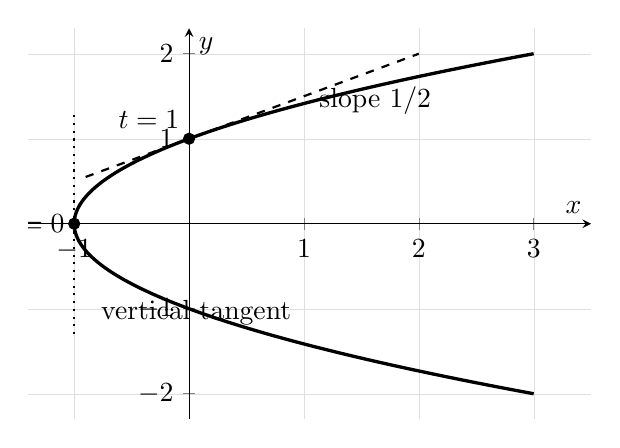
\begin{tikzpicture}
\begin{axis}[
    width=0.72\textwidth,
    height=0.54\textwidth,
    xmin=-1.4, xmax=3.5,
    ymin=-2.3, ymax=2.3,
    axis lines=middle,
    xlabel={\(x\)},
    ylabel={\(y\)},
    xtick={-1,0,1,2,3},
    ytick={-2,-1,0,1,2},
    grid=both,
    grid style={line width=.1pt, draw=gray!25},
]
\addplot[very thick, domain=-2:2, samples=160] ({x^2-1},{x});

% tangent at t=1: point (0,1), slope 1/2
\addplot[thick, dashed, domain=-0.9:2.0, samples=2] {1 + 0.5*x};

% vertical tangent at vertex
\draw[thick, dotted] (axis cs:-1,-1.3) -- (axis cs:-1,1.3);

\addplot[only marks, mark=*] coordinates {(0,1) (-1,0)};
\node[anchor=south east] at (axis cs:0,1) {\(t=1\)};
\node[anchor=east] at (axis cs:-1,0) {\(t=0\)};
\node[anchor=west] at (axis cs:1.05,1.45) {slope \(1/2\)};
\node[anchor=west] at (axis cs:-0.85,-1.05) {vertical tangent};
\end{axis}
\end{tikzpicture}
\caption{For \(x=t^2-1,\;y=t\), the slope is \(\dfrac{1}{2t}\) when \(t\neq0\).}
\label{fig:parametric-slope-sideways-parabola}
\end{figure}

The parametric formula has recovered exactly what the geometry suggests.

\paragraph{Example: slope on the circle.}
For

\[
x=\cos t,
\qquad
y=\sin t,
\]

we have

\[
\frac{dx}{dt}=-\sin t,
\qquad
\frac{dy}{dt}=\cos t.
\]

Therefore

\[
\frac{dy}{dx}
=
\frac{\cos t}{-\sin t}
=
-\cot t,
\]

as long as \(\sin t\neq0\).

At \(t=\pi/4\), the point is

\[
\left(\frac{\sqrt2}{2},\frac{\sqrt2}{2}\right),
\]

and the slope is

\[
-\cot(\pi/4)=-1.
\]

The tangent line slopes downward at \(45^\circ\), as expected on the upper right part
of the circle.

\subsection{Horizontal and vertical tangents}
\label{subsec:horizontal-vertical-tangents-parametric}

The formula

\[
\frac{dy}{dx}
=
\frac{dy/dt}{dx/dt}
\]

makes horizontal and vertical tangents easy to identify.

A horizontal tangent has slope \(0\).  This happens when

\[
\frac{dy}{dt}=0
\]

while

\[
\frac{dx}{dt}\neq0.
\]

A vertical tangent has infinite slope.  This happens when

\[
\frac{dx}{dt}=0
\]

while

\[
\frac{dy}{dt}\neq0.
\]

\begin{quote}
\textbf{Horizontal and vertical tangents for parametric curves.}

For a differentiable parametrization \(x=x(t)\), \(y=y(t)\):

\[
\boxed{
\text{horizontal tangent: } \frac{dy}{dt}=0,\quad \frac{dx}{dt}\neq0;
}
\]

\[
\boxed{
\text{vertical tangent: } \frac{dx}{dt}=0,\quad \frac{dy}{dt}\neq0.
}
\]

If both derivatives are \(0\), the test does not decide the tangent.  More work is
needed.
\end{quote}

\paragraph{Example: tangents on the unit circle.}
For

\[
x=\cos t,
\qquad
y=\sin t,
\]

we have

\[
x'(t)=-\sin t,
\qquad
y'(t)=\cos t.
\]

Horizontal tangents occur when

\[
y'(t)=\cos t=0,
\]

so

\[
t=\frac{\pi}{2},\quad \frac{3\pi}{2}.
\]

At these times,

\[
x'(t)=-\sin t\neq0.
\]

The points are

\[
(0,1)
\qquad\text{and}\qquad
(0,-1).
\]

Vertical tangents occur when

\[
x'(t)=-\sin t=0,
\]

so

\[
t=0,\quad \pi,\quad 2\pi.
\]

At these times,

\[
y'(t)=\cos t\neq0.
\]

The corresponding points are

\[
(1,0)
\qquad\text{and}\qquad
(-1,0).
\]

\begin{figure}[h]
\centering
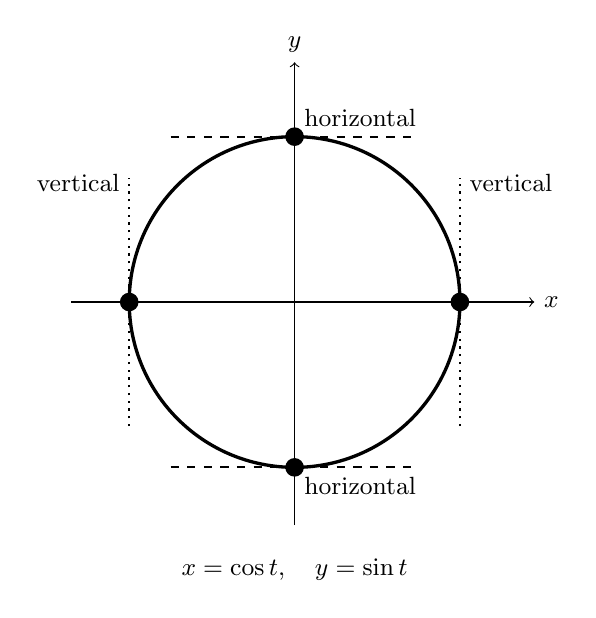
\begin{tikzpicture}[scale=2.1, every node/.style={font=\small}]
  \draw[->] (-1.35,0) -- (1.45,0) node[right] {\(x\)};
  \draw[->] (0,-1.35) -- (0,1.45) node[above] {\(y\)};

  \draw[very thick] (0,0) circle (1);

  % horizontal tangents
  \draw[thick, dashed] (-0.75,1) -- (0.75,1);
  \draw[thick, dashed] (-0.75,-1) -- (0.75,-1);

  % vertical tangents
  \draw[thick, dotted] (1,-0.75) -- (1,0.75);
  \draw[thick, dotted] (-1,-0.75) -- (-1,0.75);

  \fill (0,1) circle (1.6pt);
  \fill (0,-1) circle (1.6pt);
  \fill (1,0) circle (1.6pt);
  \fill (-1,0) circle (1.6pt);

  \node[above right] at (0,1) {horizontal};
  \node[below right] at (0,-1) {horizontal};
  \node[right] at (1,0.72) {vertical};
  \node[left] at (-1,0.72) {vertical};

  \node at (0,-1.62) {\(x=\cos t,\quad y=\sin t\)};
\end{tikzpicture}
\caption{On the unit circle, \(y'=0\) gives horizontal tangents and \(x'=0\) gives vertical tangents.}
\label{fig:circle-horizontal-vertical-tangents}
\end{figure}

This is a good example of the parametric method.  The circle is not a single graph
\(y=f(x)\), but the tangent slopes are still easy to find.

\paragraph{A warning when both derivatives vanish.}
The conditions above deliberately exclude the case

\[
x'(t)=0
\qquad\text{and}\qquad
y'(t)=0.
\]

At such a time, the moving point has zero speed.  The curve may still have a tangent,
but the simple quotient gives

\[
\frac{0}{0},
\]

which tells us nothing.

For example, let

\[
x=t^2,
\qquad
y=t^3.
\]

At \(t=0\),

\[
x'(0)=0,
\qquad
y'(0)=0.
\]

The slope formula is not legal at \(t=0\).  For \(t\neq0\),

\[
\frac{dy}{dx}
=
\frac{3t^2}{2t}
=
\frac32t.
\]

As \(t\to0\), this slope approaches \(0\).  The curve has a horizontal tangent at the
cusp, but we had to find it by a limit, not by substituting into the formula.

\begin{quote}
\textbf{Moral.}
When both \(dx/dt\) and \(dy/dt\) are zero, do not use the horizontal or vertical tangent
test blindly.  Study the nearby motion.
\end{quote}

We will meet this warning again when a curve stops, reverses, or forms a cusp.

\subsection{Concavity}
\label{subsec:parametric-concavity}

Concavity asks how the slope changes as \(x\) changes.

For an ordinary function \(y=f(x)\), we write

\[
\frac{d^2y}{dx^2}
\]

for the derivative of \(\frac{dy}{dx}\) with respect to \(x\).

For a parametric curve, \(\frac{dy}{dx}\) is first a function of \(t\).  To differentiate it
with respect to \(x\), use the same idea as before:

\[
\frac{d}{dx}
=
\frac{1}{dx/dt}\frac{d}{dt},
\]

provided \(dx/dt\neq0\).

Thus

\[
\boxed{
\frac{d^2y}{dx^2}
=
\frac{\dfrac{d}{dt}\left(\dfrac{dy}{dx}\right)}{\dfrac{dx}{dt}}.
}
\]

This formula says:

\[
\text{rate of change with respect to \(x\)}
=
\frac{\text{rate of change with respect to \(t\)}}{\text{rate of change of \(x\) with respect to \(t\)}}.
\]

It is the same slope idea one level higher.

\paragraph{Example: concavity of the sideways parabola.}
For

\[
x=t^2-1,
\qquad
y=t,
\]

we found

\[
\frac{dy}{dx}=\frac{1}{2t},
\qquad
t\neq0.
\]

Differentiate with respect to \(t\):

\[
\frac{d}{dt}\left(\frac{dy}{dx}\right)
=
\frac{d}{dt}\left(\frac{1}{2t}\right)
=
-\frac{1}{2t^2}.
\]

Since

\[
\frac{dx}{dt}=2t,
\]

we get

\[
\frac{d^2y}{dx^2}
=
\frac{-1/(2t^2)}{2t}
=
-\frac{1}{4t^3}.
\]

For \(t>0\), this is negative.  The upper branch is concave down.

For \(t<0\), this is positive.  The lower branch is concave up.

That matches the picture of

\[
x=y^2-1.
\]

The upper branch can be written as

\[
y=\sqrt{x+1},
\]

which bends downward.  The lower branch can be written as

\[
y=-\sqrt{x+1},
\]

which bends upward.

\paragraph{Example: concavity of the upper semicircle.}
Use

\[
x=\cos t,
\qquad
y=\sin t,
\qquad
0<t<\pi.
\]

This traces the upper semicircle.  We already found

\[
\frac{dy}{dx}=-\cot t.
\]

Differentiate with respect to \(t\):

\[
\frac{d}{dt}(-\cot t)=\csc^2 t.
\]

Also,

\[
\frac{dx}{dt}=-\sin t.
\]

Therefore

\[
\frac{d^2y}{dx^2}
=
\frac{\csc^2 t}{-\sin t}
=
-\frac{1}{\sin^3 t}.
\]

On \(0<t<\pi\),

\[
\sin t>0,
\]

so

\[
\frac{d^2y}{dx^2}<0.
\]

The upper semicircle is concave down everywhere.  This agrees with the graph

\[
y=\sqrt{1-x^2}.
\]

\begin{quote}
\textbf{Concavity for parametric curves.}
To find concavity:

\[
\begin{array}{ll}
\text{1.} & \text{Compute } \dfrac{dy}{dx}=\dfrac{y'(t)}{x'(t)}.\\[8pt]
\text{2.} & \text{Differentiate that expression with respect to \(t\).}\\[8pt]
\text{3.} & \text{Divide by } \dfrac{dx}{dt}.
\end{array}
\]

The result is \(\dfrac{d^2y}{dx^2}\), whenever the divisions make sense.
\end{quote}

The phrase ``whenever the divisions make sense'' is not a minor detail.  Parametric
curves can have vertical tangents, cusps, and pauses.  At such points, the algebra may
need a separate geometric check.

\subsection{Motion in the plane as a bridge to vectors}
\label{subsec:motion-plane-bridge-vectors}

Parametric equations are not only a way to draw curves.  They are also the natural
language of plane motion.

If a particle has position

\[
P(t)=(x(t),y(t)),
\]

then its horizontal and vertical velocities are

\[
x'(t)
\qquad\text{and}\qquad
y'(t).
\]

We can package them as the pair

\[
\langle x'(t),y'(t)\rangle.
\]

This pair points in the direction of motion.  Its length is the speed:

\[
\sqrt{(x'(t))^2+(y'(t))^2}.
\]

The acceleration components are

\[
x''(t)
\qquad\text{and}\qquad
y''(t),
\]

so the acceleration pair is

\[
\langle x''(t),y''(t)\rangle.
\]

This is the beginning of vector calculus, but the idea is already familiar: each
coordinate is an ordinary single-variable function of time.

\paragraph{Example: projectile motion.}
Suppose a ball is launched from height \(5\) feet with horizontal velocity \(80\) ft/s
and initial vertical velocity \(60\) ft/s.  Ignoring air resistance, its position can be
modeled by

\[
x(t)=80t,
\]

\[
y(t)=5+60t-16t^2,
\]

where \(t\) is measured in seconds.

The coordinate velocities are

\[
x'(t)=80,
\qquad
y'(t)=60-32t.
\]

The horizontal velocity is constant.  The vertical velocity decreases because gravity pulls
downward.

The acceleration components are

\[
x''(t)=0,
\qquad
y''(t)=-32.
\]

So the acceleration is

\[
\langle 0,-32\rangle,
\]

which points straight downward.

The slope of the trajectory is

\[
\frac{dy}{dx}
=
\frac{60-32t}{80}
=
\frac34-\frac25t.
\]

At \(t=0\), the slope is

\[
\frac34.
\]

At the top of the flight, the vertical velocity is \(0\):

\[
60-32t=0,
\]

so

\[
t=\frac{15}{8}.
\]

At that time,

\[
\frac{dy}{dx}=0,
\]

so the tangent is horizontal.

We can also eliminate \(t\).  Since

\[
x=80t,
\]

we have

\[
t=\frac{x}{80}.
\]

Substitute into \(y\):

\[
y=5+60\left(\frac{x}{80}\right)-16\left(\frac{x}{80}\right)^2.
\]

Simplify:

\[
y=5+\frac34x-\frac{x^2}{400}.
\]

The path is a parabola.  The parametrization tells how the ball moves along it.

\begin{figure}[h]
\centering
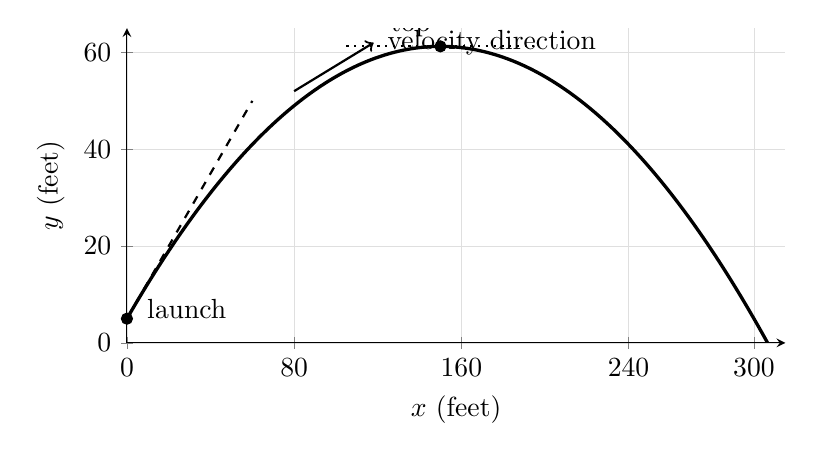
\begin{tikzpicture}
\begin{axis}[
    width=0.82\textwidth,
    height=0.46\textwidth,
    xmin=0, xmax=315,
    ymin=0, ymax=65,
    axis lines=left,
    xlabel={\(x\) (feet)},
    ylabel={\(y\) (feet)},
    xtick={0,80,160,240,300},
    ytick={0,20,40,60},
    grid=both,
    grid style={line width=.1pt, draw=gray!25},
]
\addplot[very thick, domain=0:306.5, samples=200] {5 + 0.75*x - x^2/400};

% top point: t=15/8, x=150, y=61.25
\addplot[only marks, mark=*] coordinates {(0,5) (150,61.25)};

% tangent at start slope 3/4
\addplot[thick, dashed, domain=0:60, samples=2] {5 + 0.75*x};

% horizontal tangent at top
\draw[thick, dotted] (axis cs:105,61.25) -- (axis cs:195,61.25);

% velocity arrows, drawn approximately
\draw[->, thick] (axis cs:80,52.0) -- (axis cs:118,62.0);
\node[anchor=west] at (axis cs:120,62) {velocity direction};

\node[anchor=south east] at (axis cs:150,61.25) {top};
\node[anchor=west] at (axis cs:5,7) {launch};
\end{axis}
\end{tikzpicture}
\caption{The equations \(x=80t,\;y=5+60t-16t^2\) give the path and the motion along it.}
\label{fig:parametric-projectile}
\end{figure}

This example brings several ideas together.

The Cartesian equation

\[
y=5+\frac34x-\frac{x^2}{400}
\]

shows the shape of the path.

The parametric equations

\[
x=80t,
\qquad
y=5+60t-16t^2
\]

show the motion: where the ball is at each time, how fast it moves horizontally and
vertically, when it reaches the top, and how gravity changes the vertical velocity.

\subsection{What comes next}
\label{subsec:parametric-calculus-what-next}

The derivative questions have now been answered for parametric curves.

\[
\frac{dy}{dx}
=
\frac{dy/dt}{dx/dt}
\]

gives tangent slopes, when \(dx/dt\neq0\).

\[
\frac{d^2y}{dx^2}
=
\frac{\dfrac{d}{dt}\left(\dfrac{dy}{dx}\right)}{dx/dt}
\]

gives concavity, when the divisions are valid.

But a moving point also travels a distance.  Earlier, distance came from accumulated
speed.  The same idea now applies in the plane.

If

\[
\text{speed}
=
\sqrt{(x'(t))^2+(y'(t))^2},
\]

then the length of a parametric curve should be an integral of this speed.

That is the next question:

\[
\boxed{
\text{How much length is accumulated while the point traces the curve?}
}
\]
\section{Length and area for parametric curves}
\label{sec:length-area-parametric-curves}

The last section used the coordinate rates

\[
\frac{dx}{dt}
\qquad\text{and}\qquad
\frac{dy}{dt}
\]

to find slope and concavity.  Those same rates also measure something more physical:
how much distance the moving point travels.

A parametric curve is drawn by motion.  So its length should come from speed.

\subsection{Arc length from speed}
\label{subsec:parametric-arc-length-speed}

Suppose a point has position

\[
P(t)=(x(t),y(t)),
\qquad
a\le t\le b.
\]

During a short time interval of length \(\Delta t\), the coordinate changes are
approximately

\[
\Delta x\approx x'(t)\Delta t,
\qquad
\Delta y\approx y'(t)\Delta t.
\]

The small distance traveled is therefore approximately

\[
\Delta s
\approx
\sqrt{(\Delta x)^2+(\Delta y)^2}.
\]

Substitute the approximations:

\[
\Delta s
\approx
\sqrt{\bigl(x'(t)\Delta t\bigr)^2+\bigl(y'(t)\Delta t\bigr)^2}.
\]

Thus

\[
\Delta s
\approx
\sqrt{(x'(t))^2+(y'(t))^2}\,\Delta t.
\]

The square root is the speed of the point.  Adding these small distances and passing to
the limit gives the length.

\begin{quote}
\textbf{Arc length of a parametric curve.}
If \(x'(t)\) and \(y'(t)\) are continuous on \([a,b]\), then the distance traveled by

\[
P(t)=(x(t),y(t)),
\qquad
a\le t\le b,
\]

is

\[
\boxed{
L=\int_a^b
\sqrt{\left(\frac{dx}{dt}\right)^2+
      \left(\frac{dy}{dt}\right)^2}\,dt.
}
\]

In words,

\[
\boxed{
\text{length}=\int \text{speed}\,dt.
}
\]
\end{quote}

This formula measures the distance traveled by the moving point.  If the point traces
the same curve twice, the integral counts both trips.

\paragraph{Example: a line segment.}
Let

\[
x=1+4t,
\qquad
y=2+2t,
\qquad
0\le t\le1.
\]

The point starts at

\[
(1,2)
\]

and ends at

\[
(5,4).
\]

The coordinate rates are

\[
\frac{dx}{dt}=4,
\qquad
\frac{dy}{dt}=2.
\]

So the speed is

\[
\sqrt{4^2+2^2}=\sqrt{20}=2\sqrt5.
\]

Therefore

\[
L=\int_0^1 2\sqrt5\,dt=2\sqrt5.
\]

This agrees with the distance formula:

\[
\sqrt{(5-1)^2+(4-2)^2}
=
\sqrt{16+4}
=
2\sqrt5.
\]

The arc length formula passes the simplest test.

\paragraph{Example: circumference of a circle.}
A circle of radius \(R\) can be parametrized by

\[
x=R\cos t,
\qquad
y=R\sin t,
\qquad
0\le t\le 2\pi.
\]

Then

\[
\frac{dx}{dt}=-R\sin t,
\qquad
\frac{dy}{dt}=R\cos t.
\]

The speed is

\[
\sqrt{R^2\sin^2t+R^2\cos^2t}
=
R.
\]

Thus the length is

\[
L=\int_0^{2\pi} R\,dt=2\pi R.
\]

So the familiar circumference formula comes from accumulated speed.

\begin{figure}[h]
\centering
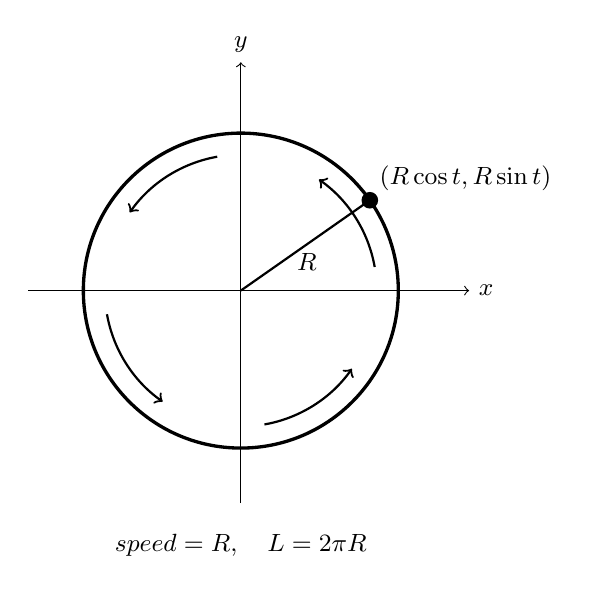
\begin{tikzpicture}[scale=2.0, every node/.style={font=\small}]
  \draw[->] (-1.35,0) -- (1.45,0) node[right] {\(x\)};
  \draw[->] (0,-1.35) -- (0,1.45) node[above] {\(y\)};

  \draw[very thick] (0,0) circle (1);

  \draw[->, thick] (0.85,0.15) arc (10:55:0.86);
  \draw[->, thick] (-0.15,0.85) arc (100:145:0.86);
  \draw[->, thick] (-0.85,-0.15) arc (190:235:0.86);
  \draw[->, thick] (0.15,-0.85) arc (280:325:0.86);

  \draw[thick] (0,0) -- ({cos(35)},{sin(35)});
  \fill ({cos(35)},{sin(35)}) circle (1.5pt);
  \node[above right] at ({cos(35)},{sin(35)}) {\((R\cos t,R\sin t)\)};
  \node at (0.42,0.18) {\(R\)};

  \node at (0,-1.62) {\(\text{speed}=R,\quad L=2\pi R\)};
\end{tikzpicture}
\caption{The circle is traced at constant speed \(R\), so its length is \(2\pi R\).}
\label{fig:parametric-circle-length}
\end{figure}

\paragraph{The graph formula as a special case.}
If a curve is already given as a graph

\[
y=f(x),
\qquad
a\le x\le b,
\]

we can parametrize it by

\[
x=t,
\qquad
y=f(t),
\qquad
a\le t\le b.
\]

Then

\[
\frac{dx}{dt}=1,
\qquad
\frac{dy}{dt}=f'(t).
\]

The parametric arc length formula becomes

\[
L=\int_a^b \sqrt{1+\bigl(f'(t)\bigr)^2}\,dt.
\]

This is exactly the arc length formula for a graph.  The parametric formula is not a new
kind of length.  It is the same length written in a more flexible language.

\begin{quote}
\textbf{Warning: geometric length versus distance traveled.}
The integral

\[
\int_a^b
\sqrt{(x'(t))^2+(y'(t))^2}\,dt
\]

counts distance traveled during the parametrized motion.

If the same geometric curve is traced twice, the integral doubles.  If the point stops
momentarily, the formula still works; a zero speed at an instant contributes no length.
\end{quote}

\subsection{Surface area from a parametrized curve of revolution}
\label{subsec:parametric-surface-area-revolution}

Earlier, surface area of revolution came from a simple small piece:

\[
dS=(\text{circumference})(\text{small arc length}).
\]

The same idea now works for a parametrized curve.

Suppose

\[
x=x(t),
\qquad
y=y(t),
\qquad
a\le t\le b,
\]

with \(y(t)\ge0\).  Rotate the curve around the \(x\)-axis.

A small arc segment has length

\[
ds=
\sqrt{\left(\frac{dx}{dt}\right)^2+
      \left(\frac{dy}{dt}\right)^2}\,dt.
\]

At height \(y(t)\), that small segment sweeps out a thin band whose circumference is

\[
2\pi y(t).
\]

So the small surface area is

\[
dS
=
2\pi y(t)\,ds.
\]

Therefore

\[
dS
=
2\pi y(t)
\sqrt{\left(\frac{dx}{dt}\right)^2+
      \left(\frac{dy}{dt}\right)^2}\,dt.
\]

\begin{quote}
\textbf{Surface area around the \(x\)-axis.}
If \(x'(t)\) and \(y'(t)\) are continuous and \(y(t)\ge0\) on \([a,b]\), then rotating the
parametric curve

\[
x=x(t),
\qquad
y=y(t)
\]

around the \(x\)-axis gives surface area

\[
\boxed{
S=
2\pi\int_a^b
y(t)
\sqrt{\left(\frac{dx}{dt}\right)^2+
      \left(\frac{dy}{dt}\right)^2}\,dt.
}
\]
\end{quote}

For rotation around the \(y\)-axis, the radius is \(x(t)\), assuming \(x(t)\ge0\).  Then

\[
\boxed{
S=
2\pi\int_a^b
x(t)
\sqrt{\left(\frac{dx}{dt}\right)^2+
      \left(\frac{dy}{dt}\right)^2}\,dt.
}
\]

More generally, the radius is always the distance from the curve to the axis of rotation.

\paragraph{Example: surface area of a sphere.}
Rotate the upper semicircle

\[
x=R\cos t,
\qquad
y=R\sin t,
\qquad
0\le t\le\pi,
\]

around the \(x\)-axis.  This produces a sphere of radius \(R\).

We already know the speed:

\[
\sqrt{\left(\frac{dx}{dt}\right)^2+
      \left(\frac{dy}{dt}\right)^2}
=
R.
\]

Therefore

\[
S=
2\pi\int_0^\pi (R\sin t)(R)\,dt.
\]

So

\[
S=2\pi R^2\int_0^\pi \sin t\,dt.
\]

Since

\[
\int_0^\pi \sin t\,dt=2,
\]

we get

\[
\boxed{
S=4\pi R^2.
}
\]

The familiar surface area of a sphere is again an accumulated band area.

\begin{figure}[h]
\centering
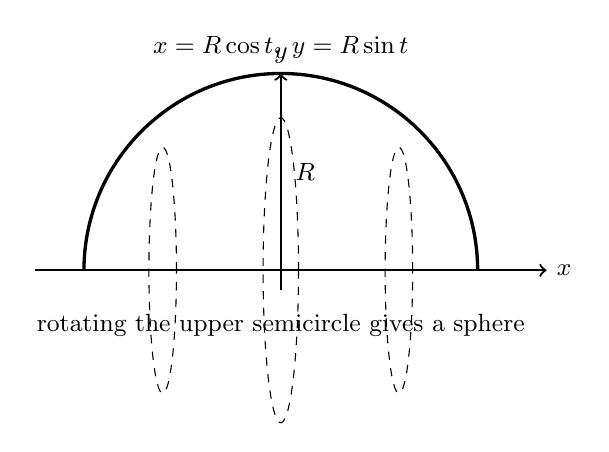
\begin{tikzpicture}[scale=1.25, every node/.style={font=\small}]
  % axes
  \draw[->, thick] (-2.5,0) -- (2.7,0) node[right] {\(x\)};
  \draw[->, thick] (0,-0.2) -- (0,2.0) node[above] {\(y\)};

  % semicircle
  \draw[very thick] (-2,0) arc (180:0:2);

  % rotation hints
  \draw[dashed] (0,0) ellipse (0.18 and 1.55);
  \draw[dashed] (-1.2,0) ellipse (0.14 and 1.25);
  \draw[dashed] (1.2,0) ellipse (0.14 and 1.25);

  % sample point/radius
  \draw[thick] (0,0) -- (0,2);
  \node[right] at (0.05,1.0) {\(R\)};

  \node[above] at (0,2.05) {\(x=R\cos t,\; y=R\sin t\)};
  \node[below] at (0,-0.35) {rotating the upper semicircle gives a sphere};
\end{tikzpicture}
\caption{The sphere is built from rotating small arc segments of the upper semicircle.}
\label{fig:sphere-from-parametric-semicircle}
\end{figure}

\begin{quote}
\textbf{Warning about the radius.}
In a surface area formula, the factor \(2\pi(\text{radius})\) must use a nonnegative
distance to the axis of rotation.

If the curve crosses the axis, or if a parametrization uses negative coordinates, check
the geometry before inserting a formula.
\end{quote}

\subsection{Area enclosed by a parametric curve}
\label{subsec:area-enclosed-parametric-curve}

Area also has a parametric form.

Start with the ordinary formula for area under a graph:

\[
A=\int y\,dx.
\]

If

\[
x=x(t),
\qquad
y=y(t),
\]

then

\[
dx=x'(t)\,dt.
\]

So whenever the curve is used as the upper boundary and \(x\) increases from left to
right, the area under the curve is

\[
\boxed{
A=\int_a^b y(t)x'(t)\,dt.
}
\]

This formula is a change of variable in disguise.  It says:

\[
\int y\,dx
=
\int y(t)\frac{dx}{dt}\,dt.
\]

\paragraph{Example: area under one arch of a parabola.}
The curve

\[
x=t,
\qquad
y=4-t^2,
\qquad
-2\le t\le 2
\]

is the graph

\[
y=4-x^2
\]

from \(x=-2\) to \(x=2\).  Since

\[
x'(t)=1,
\]

the area under the curve and above the \(x\)-axis is

\[
A=\int_{-2}^{2} (4-t^2)\,dt.
\]

Compute:

\[
A=
\left(4t-\frac{t^3}{3}\right)\Big|_{-2}^{2}
=
\left(8-\frac83\right)-\left(-8+\frac83\right).
\]

Thus

\[
A=\frac{16}{3}+\frac{16}{3}
=
\boxed{\frac{32}{3}}.
\]

The parametric formula reduces to the ordinary area formula because \(x=t\).

\paragraph{Closed curves and orientation.}
For a closed curve, the formula \(\int y\,dx\) becomes a signed quantity.  Its sign depends
on orientation.

If a simple closed curve is traced once counterclockwise, then

\[
\int y\,dx
\]

is negative.  The positive enclosed area is

\[
-\int y\,dx.
\]

A symmetric and orientation-friendly formula is

\[
\boxed{
A=
\frac12\int_a^b
\left(
x(t)y'(t)-y(t)x'(t)
\right)\,dt
}
\]

when the curve is traced once counterclockwise.

If the curve is traced clockwise, this integral is negative, and the positive area is its
absolute value.

\begin{quote}
\textbf{Area enclosed by a parametric curve.}
For a simple closed curve traced once counterclockwise,

\[
\boxed{
A=
\int_a^b x(t)y'(t)\,dt
=
-\int_a^b y(t)x'(t)\,dt
=
\frac12\int_a^b
\bigl(x(t)y'(t)-y(t)x'(t)\bigr)\,dt.
}
\]

If the orientation is clockwise, these signed formulas change sign.
\end{quote}

\paragraph{Example: area of an ellipse.}
Parametrize the ellipse

\[
\frac{x^2}{a^2}+\frac{y^2}{b^2}=1
\]

by

\[
x=a\cos t,
\qquad
y=b\sin t,
\qquad
0\le t\le2\pi.
\]

This traces the ellipse counterclockwise.

We use

\[
A=
\frac12\int_0^{2\pi}
\bigl(x(t)y'(t)-y(t)x'(t)\bigr)\,dt.
\]

Compute the derivatives:

\[
x'(t)=-a\sin t,
\qquad
y'(t)=b\cos t.
\]

Then

\[
x(t)y'(t)-y(t)x'(t)
=
(a\cos t)(b\cos t)-(b\sin t)(-a\sin t).
\]

So

\[
x(t)y'(t)-y(t)x'(t)
=
ab\cos^2t+ab\sin^2t
=
ab.
\]

Therefore

\[
A=
\frac12\int_0^{2\pi} ab\,dt
=
\frac12 ab(2\pi)
=
\boxed{\pi ab}.
\]

When \(a=b=R\), this becomes

\[
\pi R^2,
\]

the area of a circle.

\begin{figure}[h]
\centering
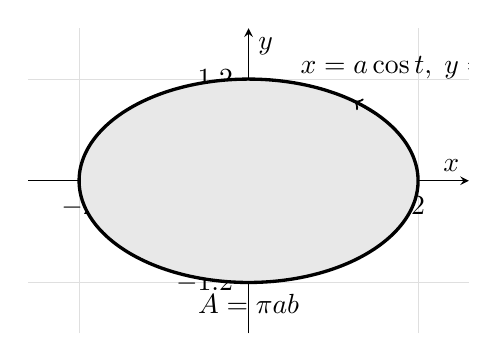
\begin{tikzpicture}
\begin{axis}[
    width=0.72\textwidth,
    height=0.45\textwidth,
    xmin=-2.6, xmax=2.6,
    ymin=-1.8, ymax=1.8,
    axis lines=middle,
    xlabel={\(x\)},
    ylabel={\(y\)},
    xtick={-2,0,2},
    ytick={-1.2,0,1.2},
    axis equal image,
    grid=both,
    grid style={line width=.1pt, draw=gray!25},
]
\addplot[domain=0:360, samples=240, fill=gray!18, draw=none]
    ({2*cos(x)},{1.2*sin(x)}) \closedcycle;
\addplot[very thick, domain=0:360, samples=240]
    ({2*cos(x)},{1.2*sin(x)});
\draw[->, thick] (axis cs:1.5,0.79) -- (axis cs:1.25,0.94);
\node[anchor=west] at (axis cs:0.5,1.35) {\(x=a\cos t,\;y=b\sin t\)};
\node at (axis cs:0,-1.45) {\(A=\pi ab\)};
\end{axis}
\end{tikzpicture}
\caption{The counterclockwise parametrization of an ellipse gives the area \(\pi ab\).}
\label{fig:parametric-ellipse-area}
\end{figure}

\begin{quote}
\textbf{Warning about repeated tracing.}
The area formulas count with the parametrization.

If a curve is traced twice counterclockwise, the signed area integral doubles.  If one
part is traced clockwise and another counterclockwise, cancellation can occur.

Before using a closed-curve area formula, check how many times the curve is traced and
in which direction.
\end{quote}

\subsection{Cycloids and rolling motion}
\label{subsec:cycloids-rolling-motion}

A wheel rolling along a road draws one of the most beautiful curves in calculus.

Fix a point on the rim of a circle of radius \(R\).  Let the circle roll to the right without
slipping.  The point on the rim traces a curve called a \emph{cycloid}.

If \(t\) is the angle through which the wheel has rotated, then the center of the wheel has
moved horizontally a distance

\[
Rt.
\]

Relative to the center, the point on the rim has coordinates

\[
(-R\sin t,\,-R\cos t).
\]

Since the center is at

\[
(Rt,R),
\]

the point on the rim is

\[
\boxed{
x=R(t-\sin t),
\qquad
y=R(1-\cos t).
}
\]

One arch of the cycloid occurs for

\[
0\le t\le 2\pi.
\]

At \(t=0\), the point is on the ground:

\[
(x,y)=(0,0).
\]

At \(t=2\pi\), the point returns to the ground:

\[
(x,y)=(2\pi R,0).
\]

\begin{figure}[h]
\centering
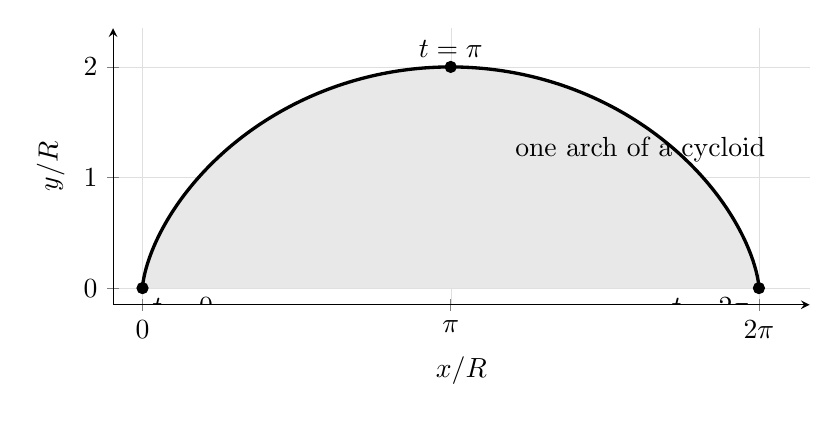
\begin{tikzpicture}
\begin{axis}[
    width=0.86\textwidth,
    height=0.42\textwidth,
    xmin=-0.3, xmax=6.8,
    ymin=-0.15, ymax=2.35,
    axis lines=left,
    xlabel={\(x/R\)},
    ylabel={\(y/R\)},
    xtick={0,3.14159,6.28318},
    xticklabels={\(0\),\(\pi\),\(2\pi\)},
    ytick={0,1,2},
    grid=both,
    grid style={line width=.1pt, draw=gray!25},
]
\addplot[domain=0:6.283185, samples=240, fill=gray!18, draw=none]
    ({x - sin(deg(x))},{1 - cos(deg(x))}) \closedcycle;
\addplot[very thick, domain=0:6.283185, samples=240]
    ({x - sin(deg(x))},{1 - cos(deg(x))});
\addplot[only marks, mark=*] coordinates {(0,0) (3.14159,2) (6.28318,0)};
\node[anchor=south] at (axis cs:3.14159,2) {\(t=\pi\)};
\node[anchor=north west] at (axis cs:0,0) {\(t=0\)};
\node[anchor=north east] at (axis cs:6.28318,0) {\(t=2\pi\)};
\node[anchor=west] at (axis cs:3.7,1.25) {one arch of a cycloid};
\end{axis}
\end{tikzpicture}
\caption{A point on a rolling wheel traces a cycloid.  The picture is scaled by \(R\).}
\label{fig:cycloid-one-arch}
\end{figure}

\paragraph{Length of one arch.}
Differentiate:

\[
\frac{dx}{dt}=R(1-\cos t),
\qquad
\frac{dy}{dt}=R\sin t.
\]

The speed is

\[
\sqrt{R^2(1-\cos t)^2+R^2\sin^2t}.
\]

Factor out \(R\):

\[
\text{speed}
=
R\sqrt{(1-\cos t)^2+\sin^2t}.
\]

Simplify the expression inside the square root:

\[
(1-\cos t)^2+\sin^2t
=
1-2\cos t+\cos^2t+\sin^2t
=
2-2\cos t.
\]

Using

\[
1-\cos t=2\sin^2\left(\frac t2\right),
\]

we get

\[
2-2\cos t=4\sin^2\left(\frac t2\right).
\]

On \(0\le t\le2\pi\),

\[
\sin\left(\frac t2\right)\ge0.
\]

Therefore

\[
\text{speed}=2R\sin\left(\frac t2\right).
\]

The length of one arch is

\[
L=\int_0^{2\pi}2R\sin\left(\frac t2\right)\,dt.
\]

Compute:

\[
L
=
2R\left[-2\cos\left(\frac t2\right)\right]_0^{2\pi}.
\]

So

\[
L
=
-4R\left(\cos\pi-\cos0\right)
=
-4R(-1-1)
=
\boxed{8R}.
\]

This is a surprising answer.  The width of one arch is \(2\pi R\), but the length of the
curved arch is \(8R\).

\paragraph{Area under one arch.}
Since

\[
x'(t)=R(1-\cos t)
\]

and

\[
y(t)=R(1-\cos t),
\]

the area under one arch is

\[
A=\int_0^{2\pi} y(t)x'(t)\,dt
=
R^2\int_0^{2\pi}(1-\cos t)^2\,dt.
\]

Expand:

\[
(1-\cos t)^2=1-2\cos t+\cos^2t.
\]

Therefore

\[
A=
R^2\int_0^{2\pi}
\left(1-2\cos t+\cos^2t\right)\,dt.
\]

Now

\[
\int_0^{2\pi}1\,dt=2\pi,
\]

\[
\int_0^{2\pi}\cos t\,dt=0,
\]

and

\[
\int_0^{2\pi}\cos^2t\,dt=\pi.
\]

Thus

\[
A=R^2(2\pi+\pi)=\boxed{3\pi R^2}.
\]

One arch of a cycloid encloses exactly three times the area of the rolling circle.

\begin{quote}
\textbf{Cycloid facts.}
For the cycloid

\[
x=R(t-\sin t),
\qquad
y=R(1-\cos t),
\qquad
0\le t\le2\pi,
\]

one arch has

\[
\boxed{L=8R}
\qquad\text{and}\qquad
\boxed{A=3\pi R^2}.
\]
\end{quote}

At the endpoints of the arch,

\[
x'(t)=0
\qquad\text{and}\qquad
y'(t)=0.
\]

The point on the wheel momentarily stops when it touches the ground.  The curve has
cusps there.  This is exactly the kind of behavior that parametric equations handle
naturally: the formulas describe not only the curve, but also the motion that creates it.

The next coordinate system also comes from motion, but of a different kind.  Instead of
following horizontal and vertical coordinates, we measure a point by how far it is from
the origin and which direction it lies.

\section{Polar coordinates}
\label{sec:polar-coordinates}

Cartesian coordinates answer two questions:

\[
\text{How far left or right?}
\qquad
\text{How far up or down?}
\]

Polar coordinates answer different questions:

\[
\text{How far from the origin?}
\qquad
\text{At what angle?}
\]

This is often the natural language of rotation, spirals, circular motion, and orbits.

\subsection{Distance and angle as coordinates}
\label{subsec:distance-angle-coordinates}

Fix an origin \(O\) and a positive \(x\)-axis.  A point \(P\) can be described by:

\[
r=\text{directed distance from the origin},
\]

and

\[
\theta=\text{angle measured from the positive \(x\)-axis}.
\]

The pair

\[
(r,\theta)
\]

is called a pair of \emph{polar coordinates}.

If \(r>0\), the point lies \(r\) units from the origin in the direction of angle \(\theta\).

\begin{figure}[h]
\centering
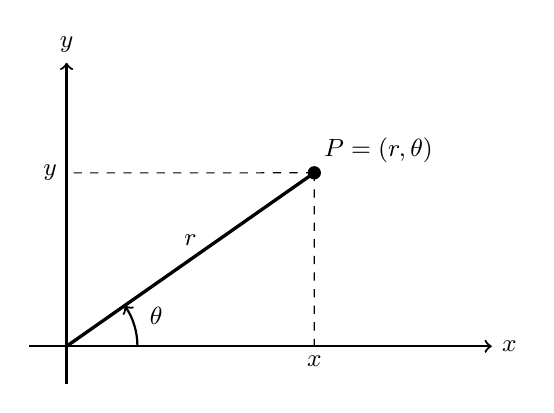
\begin{tikzpicture}[scale=1.2, every node/.style={font=\small}]
  % axes
  \draw[->, thick] (-0.4,0) -- (4.5,0) node[right] {\(x\)};
  \draw[->, thick] (0,-0.4) -- (0,3.0) node[above] {\(y\)};

  % point
  \coordinate (P) at ({3.2*cos(35)},{3.2*sin(35)});
  \draw[very thick] (0,0) -- (P);
  \fill (P) circle (2pt);
  \node[above right] at (P) {\(P=(r,\theta)\)};

  % angle
  \draw[->, thick] (0.75,0) arc (0:35:0.75);
  \node at (0.95,0.32) {\(\theta\)};

  % radius label
  \node[above] at ({1.6*cos(35)},{1.6*sin(35)+0.05}) {\(r\)};

  % projections
  \draw[dashed] (P) -- ({3.2*cos(35)},0);
  \draw[dashed] (P) -- (0,{3.2*sin(35)});
  \node[below] at ({3.2*cos(35)},0) {\(x\)};
  \node[left] at (0,{3.2*sin(35)}) {\(y\)};
\end{tikzpicture}
\caption{Polar coordinates describe a point by distance from the origin and angle from the positive \(x\)-axis.}
\label{fig:polar-coordinate-point}
\end{figure}

The angle \(\theta\) is measured in radians unless stated otherwise.  Positive angles are
measured counterclockwise.  Negative angles are measured clockwise.

For example,

\[
\left(2,\frac{\pi}{3}\right)
\]

means: go distance \(2\) from the origin in the direction \(60^\circ\) above the positive
\(x\)-axis.

\paragraph{Polar coordinates are not unique.}
The point

\[
\left(2,\frac{\pi}{3}\right)
\]

is the same as

\[
\left(2,\frac{\pi}{3}+2\pi\right),
\]

because adding \(2\pi\) makes one full turn.

More generally,

\[
(r,\theta)
\]

and

\[
(r,\theta+2k\pi)
\]

represent the same point for any integer \(k\).

There is another source of nonuniqueness.  A negative \(r\) means that the point is
plotted in the opposite direction from the angle \(\theta\).  Thus

\[
(-r,\theta)
\]

represents the same point as

\[
(r,\theta+\pi).
\]

For example,

\[
\left(-2,\frac{\pi}{3}\right)
\]

is the same point as

\[
\left(2,\frac{4\pi}{3}\right).
\]

The origin is even more nonunique.  It can be written as

\[
(0,\theta)
\]

for every angle \(\theta\).

\begin{quote}
\textbf{Polar warning.}
A Cartesian point usually has one coordinate pair.

A polar point has many coordinate pairs:

\[
(r,\theta)=(r,\theta+2\pi)=(-r,\theta+\pi)=\cdots.
\]

This nonuniqueness is useful, but it also makes polar graphs easy to misread.
\end{quote}

\subsection{Converting between polar and Cartesian coordinates}
\label{subsec:polar-cartesian-conversion}

The right triangle in Figure \ref{fig:polar-coordinate-point} gives the conversion formulas.

If a point has polar coordinates \((r,\theta)\), then

\[
\boxed{
x=r\cos\theta,
\qquad
y=r\sin\theta.
}
\]

Conversely, if a point has Cartesian coordinates \((x,y)\), then

\[
\boxed{
r^2=x^2+y^2.
}
\]

When \(r>0\), the angle satisfies

\[
\boxed{
\tan\theta=\frac{y}{x}
}
\]

when \(x\neq0\).  The quadrant must be chosen from the signs of \(x\) and \(y\).

\paragraph{Example: polar to Cartesian.}
Convert

\[
\left(2,\frac{\pi}{6}\right)
\]

to Cartesian coordinates.

Use

\[
x=r\cos\theta,
\qquad
y=r\sin\theta.
\]

Then

\[
x=2\cos\frac{\pi}{6}=2\cdot\frac{\sqrt3}{2}=\sqrt3,
\]

and

\[
y=2\sin\frac{\pi}{6}=2\cdot\frac12=1.
\]

So

\[
\boxed{
\left(2,\frac{\pi}{6}\right)=(\sqrt3,1).
}
\]

\paragraph{Example: Cartesian to polar.}
Convert

\[
(-1,\sqrt3)
\]

to polar coordinates with \(r>0\) and \(0\le\theta<2\pi\).

First,

\[
r^2=(-1)^2+(\sqrt3)^2=1+3=4,
\]

so

\[
r=2.
\]

Next,

\[
\tan\theta=\frac{\sqrt3}{-1}=-\sqrt3.
\]

The point lies in Quadrant II, so

\[
\theta=\frac{2\pi}{3}.
\]

Thus one polar representation is

\[
\boxed{
(-1,\sqrt3)=\left(2,\frac{2\pi}{3}\right).
}
\]

Other representations include

\[
\left(2,\frac{2\pi}{3}+2\pi\right)
\]

and

\[
\left(-2,-\frac{\pi}{3}\right).
\]

\paragraph{Example: a circle in polar form.}
Convert

\[
r=2\cos\theta
\]

to a Cartesian equation.

Multiply both sides by \(r\):

\[
r^2=2r\cos\theta.
\]

Now use

\[
r^2=x^2+y^2
\]

and

\[
r\cos\theta=x.
\]

So

\[
x^2+y^2=2x.
\]

Complete the square:

\[
x^2-2x+y^2=0,
\]

\[
(x-1)^2+y^2=1.
\]

Thus

\[
\boxed{
r=2\cos\theta
}
\]

is the circle centered at \((1,0)\) with radius \(1\).

This example is important.  A circle that is slightly awkward in Cartesian coordinates may
be very simple in polar coordinates.

\paragraph{Example: a line through the origin.}
The equation

\[
\theta=\frac{\pi}{4}
\]

means all points whose direction from the origin is \(45^\circ\).  This is the line

\[
y=x.
\]

If we allow \(r\) to be negative as well as positive, then one equation

\[
\theta=\frac{\pi}{4}
\]

traces the whole line.  Positive \(r\) gives the ray in Quadrant I.  Negative \(r\) gives
the opposite ray in Quadrant III.

\subsection{Polar graphs}
\label{subsec:polar-graphs}

A polar equation usually gives \(r\) as a function of \(\theta\):

\[
r=f(\theta).
\]

For each angle \(\theta\), we compute the distance \(r\), then plot the point

\[
(r,\theta).
\]

But there is a second way to see the same graph.  Every polar equation

\[
r=f(\theta)
\]

is automatically a parametric curve:

\[
\boxed{
x=f(\theta)\cos\theta,
\qquad
y=f(\theta)\sin\theta.
}
\]

The angle \(\theta\) is the parameter.

This is why polar coordinates belong in the same chapter as parametric curves.  A polar
graph is a curve traced by a rotating ray.

\paragraph{Example: the circle \(r=2\).}
The equation

\[
r=2
\]

means that every point on the graph has distance \(2\) from the origin.  Therefore the
graph is the circle

\[
x^2+y^2=4.
\]

In parametric form,

\[
x=2\cos\theta,
\qquad
y=2\sin\theta.
\]

So the polar circle is the same circle parametrization we already know.

\paragraph{Example: the spiral \(r=\theta\).}
The equation

\[
r=\theta,
\qquad
\theta\ge0,
\]

says that the distance from the origin grows at the same rate as the angle.

At

\[
\theta=0,
\]

we have

\[
r=0.
\]

At

\[
\theta=2\pi,
\]

we have

\[
r=2\pi.
\]

After one full turn, the point is farther from the origin.  After another full turn, it is
farther still.  The curve is a spiral.

This curve is called an \emph{Archimedean spiral}.  More generally,

\[
r=a\theta
\]

has radius increasing linearly with angle.

\begin{figure}[h]
\centering
\begin{minipage}{0.45\textwidth}
\centering
\begin{tikzpicture}
\begin{axis}[
    width=\textwidth,
    height=\textwidth,
    xmin=-2.3, xmax=2.3,
    ymin=-2.3, ymax=2.3,
    axis lines=middle,
    xtick={-2,0,2},
    ytick={-2,0,2},
    axis equal image,
    grid=both,
    grid style={line width=.1pt, draw=gray!25},
    title={\(r=2\)}
]
\addplot[very thick, domain=0:6.283185, samples=200]
    ({2*cos(deg(x))},{2*sin(deg(x))});
\end{axis}
\end{tikzpicture}
\end{minipage}
\hfill
\begin{minipage}{0.45\textwidth}
\centering
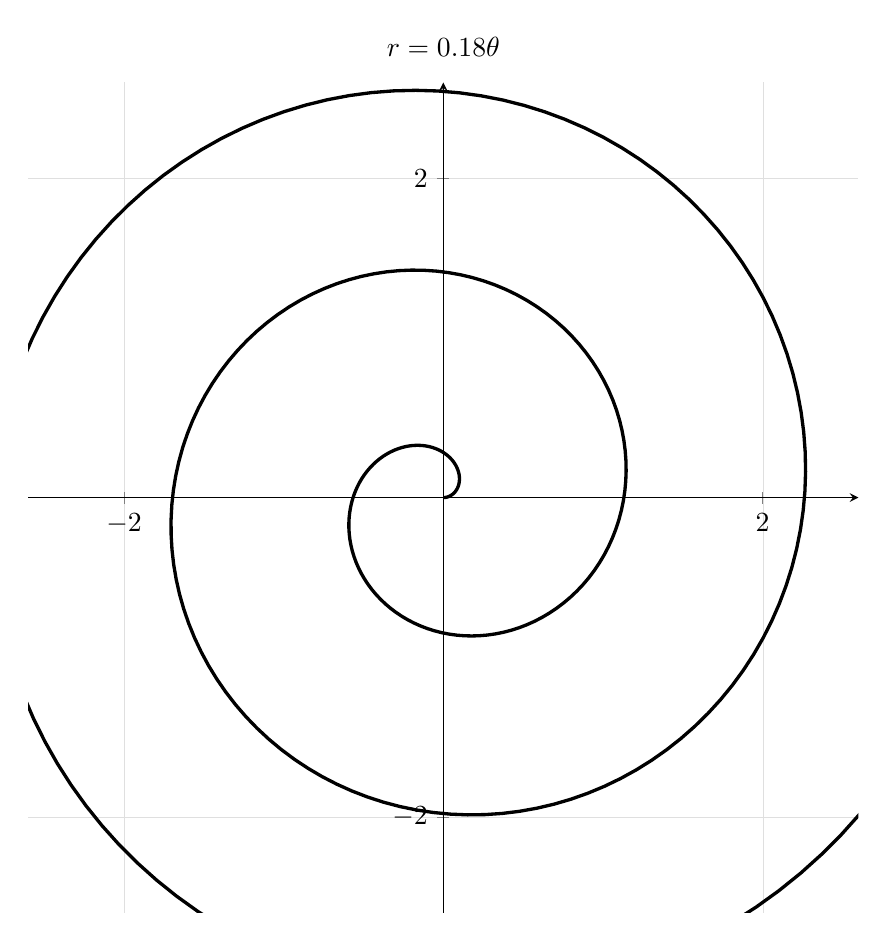
\begin{tikzpicture}
\begin{axis}[
    width=\textwidth,
    height=\textwidth,
    xmin=-2.6, xmax=2.6,
    ymin=-2.6, ymax=2.6,
    axis lines=middle,
    xtick={-2,0,2},
    ytick={-2,0,2},
    axis equal image,
    grid=both,
    grid style={line width=.1pt, draw=gray!25},
    title={\(r=0.18\theta\)}
]
\addplot[very thick, domain=0:18.8495559, samples=350]
    ({0.18*x*cos(deg(x))},{0.18*x*sin(deg(x))});
\end{axis}
\end{tikzpicture}
\end{minipage}
\caption{A constant radius gives a circle.  A radius growing with angle gives a spiral.}
\label{fig:circle-and-spiral-polar}
\end{figure}

\paragraph{How to sketch a polar graph.}
A polar graph is easier to sketch if we ask four questions.

\begin{center}
\begin{tabular}{c|p{0.62\textwidth}}
\textbf{Question} & \textbf{Why it helps} \\ \hline
What values of \(\theta\) are needed? & The curve may be traced once on a smaller interval than \(0\le\theta\le2\pi\). \\[3pt]
When is \(r=0\)? & These angles send the curve through the origin. \\[3pt]
When is \(r\) largest or smallest? & These angles locate the outermost and innermost points. \\[3pt]
Can \(r\) be negative? & Negative \(r\) plots the point in the opposite direction.
\end{tabular}
\end{center}

The last question is the one most students forget.

\begin{quote}
\textbf{Negative \(r\) is not an error.}
If a polar equation gives \(r<0\), plot the point by turning the ray through angle
\(\theta\), then moving \(|r|\) units in the opposite direction.

Equivalently,

\[
(r,\theta)=(-r,\theta+\pi).
\]
\end{quote}

\subsection{Circles, spirals, roses, and limacons}
\label{subsec:polar-families}

Polar coordinates make several families of curves appear with simple equations.

\subsubsection*{Circles}

The equation

\[
r=a
\]

is the circle centered at the origin with radius \(a\), assuming \(a>0\).

The equation

\[
r=2a\cos\theta
\]

is a circle centered at \((a,0)\) with radius \(a\).  To see this, multiply by \(r\):

\[
r^2=2ar\cos\theta.
\]

Convert:

\[
x^2+y^2=2ax.
\]

Complete the square:

\[
(x-a)^2+y^2=a^2.
\]

Similarly,

\[
r=2a\sin\theta
\]

is the circle centered at \((0,a)\) with radius \(a\).

\begin{figure}[h]
\centering
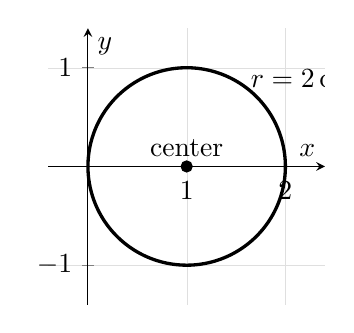
\begin{tikzpicture}
\begin{axis}[
    width=0.58\textwidth,
    height=0.42\textwidth,
    xmin=-0.4, xmax=2.4,
    ymin=-1.4, ymax=1.4,
    axis lines=middle,
    xlabel={\(x\)},
    ylabel={\(y\)},
    xtick={0,1,2},
    ytick={-1,0,1},
    axis equal image,
    grid=both,
    grid style={line width=.1pt, draw=gray!25},
]
\addplot[very thick, domain=-1.5707963:1.5707963, samples=180]
    ({2*cos(deg(x))*cos(deg(x))},{2*cos(deg(x))*sin(deg(x))});
\addplot[only marks, mark=*] coordinates {(1,0)};
\node[anchor=south] at (axis cs:1,0) {center};
\node[anchor=west] at (axis cs:1.55,0.9) {\(r=2\cos\theta\)};
\end{axis}
\end{tikzpicture}
\caption{The polar equation \(r=2\cos\theta\) is the circle \((x-1)^2+y^2=1\).}
\label{fig:polar-circle-offset}
\end{figure}

\subsubsection*{Spirals}

The equation

\[
r=a\theta,
\qquad
a>0,
\]

is an Archimedean spiral.  Each full turn increases the radius by

\[
2\pi a.
\]

Indeed, increasing \(\theta\) by \(2\pi\) changes \(r\) by

\[
a(\theta+2\pi)-a\theta=2\pi a.
\]

So the turns of the spiral are evenly spaced.

This is different from exponential spirals, where the radius multiplies after each turn.
Polar coordinates make both kinds natural because the angle is already part of the
coordinate system.

\subsubsection*{Roses}

Equations such as

\[
r=a\cos(n\theta)
\qquad\text{or}\qquad
r=a\sin(n\theta)
\]

produce flower-shaped curves called \emph{roses}.

For example,

\[
r=2\cos(3\theta)
\]

has three petals.  The factor \(3\theta\) makes the radius oscillate three times as the
angle runs from \(0\) to \(2\pi\).

\begin{figure}[h]
\centering
\begin{minipage}{0.45\textwidth}
\centering
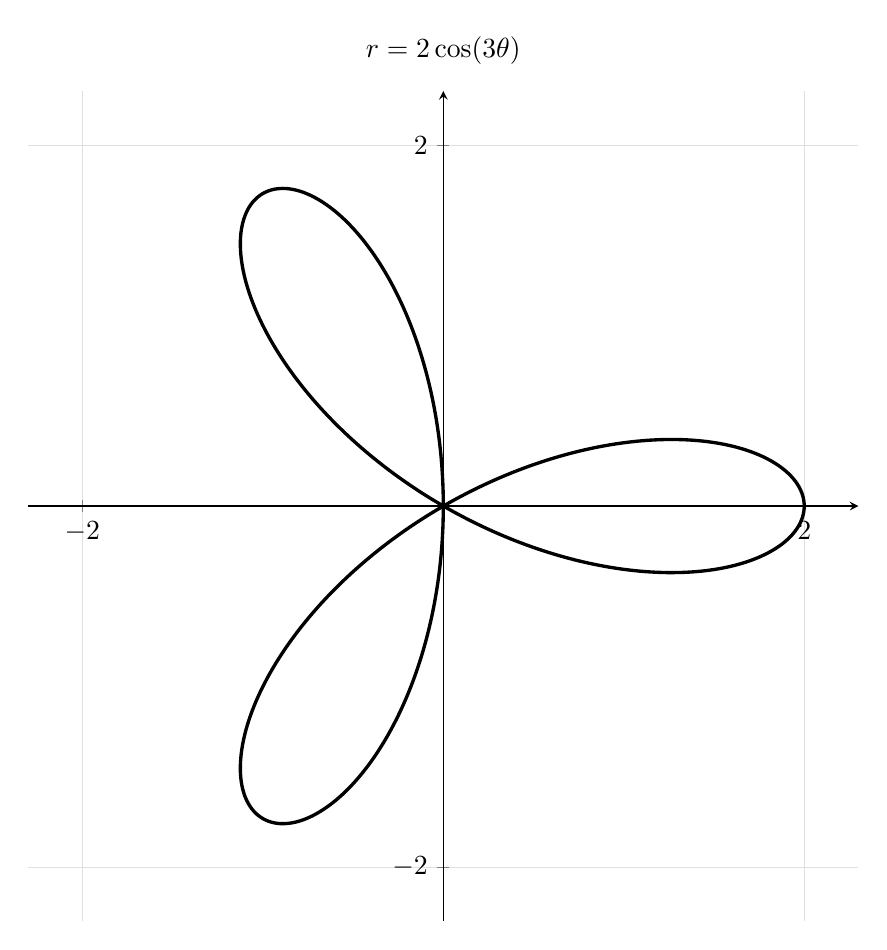
\begin{tikzpicture}
\begin{axis}[
    width=\textwidth,
    height=\textwidth,
    xmin=-2.3, xmax=2.3,
    ymin=-2.3, ymax=2.3,
    axis lines=middle,
    xtick={-2,0,2},
    ytick={-2,0,2},
    axis equal image,
    grid=both,
    grid style={line width=.1pt, draw=gray!25},
    title={\(r=2\cos(3\theta)\)}
]
\addplot[very thick, domain=0:6.283185, samples=500]
    ({2*cos(deg(3*x))*cos(deg(x))},{2*cos(deg(3*x))*sin(deg(x))});
\end{axis}
\end{tikzpicture}
\end{minipage}
\hfill
\begin{minipage}{0.45\textwidth}
\centering
\begin{tikzpicture}
\begin{axis}[
    width=\textwidth,
    height=\textwidth,
    xmin=-2.3, xmax=2.3,
    ymin=-2.3, ymax=2.3,
    axis lines=middle,
    xtick={-2,0,2},
    ytick={-2,0,2},
    axis equal image,
    grid=both,
    grid style={line width=.1pt, draw=gray!25},
    title={\(r=1+\cos\theta\)}
]
\addplot[very thick, domain=0:6.283185, samples=400]
    ({(1+cos(deg(x)))*cos(deg(x))},{(1+cos(deg(x)))*sin(deg(x))});
\end{axis}
\end{tikzpicture}
\end{minipage}
\caption{Rose curves and limacons are simple in polar coordinates but awkward in Cartesian coordinates.}
\label{fig:rose-cardioid-polar}
\end{figure}

A useful rule of thumb is:

\begin{center}
\begin{tabular}{c|c}
\textbf{rose equation} & \textbf{number of petals} \\ \hline
\(r=a\cos(n\theta)\) or \(r=a\sin(n\theta)\), \(n\) odd & \(n\) petals \\[3pt]
\(r=a\cos(n\theta)\) or \(r=a\sin(n\theta)\), \(n\) even & \(2n\) petals
\end{tabular}
\end{center}

This rule describes the usual full polar graph.  The reason comes from periodicity and
negative \(r\).  When \(r\) becomes negative, the graph is not discarded; it is plotted in
the opposite direction, which may create another petal or retrace one already drawn.

\subsubsection*{Limacons and cardioids}

Equations of the form

\[
r=a+b\cos\theta
\qquad\text{or}\qquad
r=a+b\sin\theta
\]

produce curves called \emph{limacons}.  The name comes from a word for snail, and the
curves often have a rounded shell-like shape.

The special case

\[
a=b
\]

is called a \emph{cardioid}.  For example,

\[
r=1+\cos\theta
\]

is a cardioid.  It has a cusp at the origin because

\[
r=1+\cos\pi=0.
\]

The largest radius occurs at

\[
\theta=0,
\]

where

\[
r=2.
\]

So the curve points to the right and pinches at the origin on the left.

If \(b>a>0\), then \(r=a+b\cos\theta\) becomes negative for some angles.  The graph
develops an inner loop.

\begin{figure}[h]
\centering
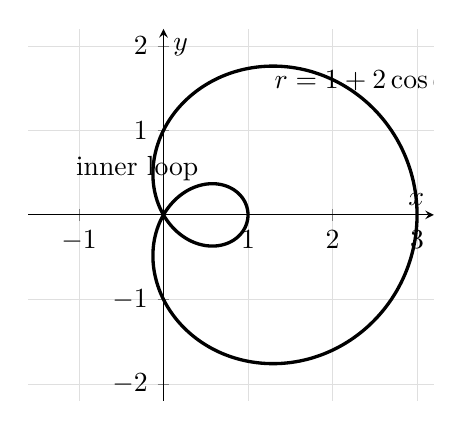
\begin{tikzpicture}
\begin{axis}[
    width=0.64\textwidth,
    height=0.52\textwidth,
    xmin=-1.6, xmax=3.2,
    ymin=-2.2, ymax=2.2,
    axis lines=middle,
    xlabel={\(x\)},
    ylabel={\(y\)},
    xtick={-1,0,1,2,3},
    ytick={-2,-1,0,1,2},
    axis equal image,
    grid=both,
    grid style={line width=.1pt, draw=gray!25},
]
\addplot[very thick, domain=0:6.283185, samples=500]
    ({(1+2*cos(deg(x)))*cos(deg(x))},{(1+2*cos(deg(x)))*sin(deg(x))});
\node[anchor=west] at (axis cs:1.2,1.6) {\(r=1+2\cos\theta\)};
\node[anchor=west] at (axis cs:-1.15,0.55) {inner loop};
\end{axis}
\end{tikzpicture}
\caption{When \(r=1+2\cos\theta\), negative values of \(r\) create an inner loop.}
\label{fig:limacon-inner-loop}
\end{figure}

\begin{quote}
\textbf{Why polar coordinates matter.}
Curves involving circles, rotations, angles, or distance from a fixed point often have
simple polar equations and complicated Cartesian equations.

Polar coordinates do not replace Cartesian coordinates.  They give us another language,
better suited to radial and angular geometry.
\end{quote}

A polar equation

\[
r=f(\theta)
\]

is already a parametric curve:

\[
x=f(\theta)\cos\theta,
\qquad
y=f(\theta)\sin\theta.
\]

So the calculus we built for parametric curves should also give slopes, areas, and lengths
for polar curves.  The next section does exactly that.
\section{Calculus in polar coordinates}
\label{sec:calculus-polar-coordinates}

The last section ended with one important observation:

\[
r=f(\theta)
\]

is already a parametric curve, because

\[
x=f(\theta)\cos\theta,
\qquad
y=f(\theta)\sin\theta.
\]

So polar calculus is not a new kind of calculus.  It is parametric calculus with the angle
\(\theta\) as the parameter.

The polar picture, however, gives new geometry.  A small change in \(\theta\) sweeps
out a small sector.  A small change in \(r\) moves the point in or out along a ray.  That
is why the formulas for slope, area, and length look different from the ones for ordinary
graphs.

\subsection{Slope of a polar curve}
\label{subsec:slope-polar-curve}

Start with a simple polar curve:

\[
r=\theta,
\qquad
\theta\ge0.
\]

This is a spiral.  It is not naturally a graph \(y=f(x)\).  But it is naturally a moving point:

\[
x=\theta\cos\theta,
\qquad
y=\theta\sin\theta.
\]

The slope is still

\[
\frac{dy}{dx}.
\]

Because both \(x\) and \(y\) depend on \(\theta\), we use the parametric slope formula:

\[
\frac{dy}{dx}
=
\frac{dy/d\theta}{dx/d\theta}.
\]

For the spiral,

\[
\frac{dx}{d\theta}
=
\cos\theta-\theta\sin\theta,
\]

and

\[
\frac{dy}{d\theta}
=
\sin\theta+\theta\cos\theta.
\]

Therefore

\[
\frac{dy}{dx}
=
\frac{\sin\theta+\theta\cos\theta}
{\cos\theta-\theta\sin\theta}.
\]

At

\[
\theta=\pi,
\]

the point is

\[
r=\pi,
\]

so

\[
x=\pi\cos\pi=-\pi,
\qquad
y=\pi\sin\pi=0.
\]

The slope is

\[
\frac{\sin\pi+\pi\cos\pi}
{\cos\pi-\pi\sin\pi}
=
\frac{0-\pi}{-1-0}
=
\pi.
\]

So the tangent line to the spiral at the point \((-\pi,0)\) has slope \(\pi\).

\begin{figure}[h]
\centering
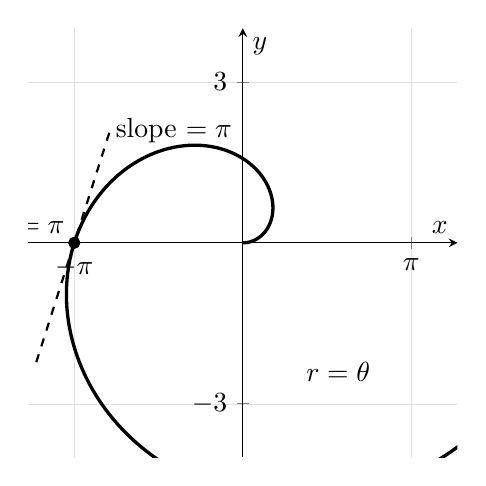
\begin{tikzpicture}
\begin{axis}[
    width=0.74\textwidth,
    height=0.58\textwidth,
    xmin=-4.0, xmax=4.0,
    ymin=-4.0, ymax=4.0,
    axis lines=middle,
    xlabel={\(x\)},
    ylabel={\(y\)},
    xtick={-3.14159,0,3.14159},
    xticklabels={\(-\pi\),\(0\),\(\pi\)},
    ytick={-3,0,3},
    axis equal image,
    grid=both,
    grid style={line width=.1pt, draw=gray!25},
]
\addplot[very thick, domain=0:6.283185, samples=350]
    ({x*cos(deg(x))},{x*sin(deg(x))});

% tangent at theta=pi: point (-pi,0), slope pi
\addplot[thick, dashed, domain=-3.85:-2.45, samples=2]
    {3.14159*(x+3.14159)};

\addplot[only marks, mark=*] coordinates {(-3.14159,0)};
\node[anchor=south east] at (axis cs:-3.14159,0) {\(\theta=\pi\)};
\node[anchor=west] at (axis cs:-2.55,2.1) {slope \(=\pi\)};
\node[anchor=west] at (axis cs:1.0,-2.4) {\(r=\theta\)};
\end{axis}
\end{tikzpicture}
\caption{A polar graph is a parametric curve with \(\theta\) as the parameter.}
\label{fig:polar-spiral-slope}
\end{figure}

Now do the same calculation for a general polar curve

\[
r=f(\theta).
\]

To keep the notation light, write

\[
r=r(\theta).
\]

Then

\[
x=r\cos\theta,
\qquad
y=r\sin\theta.
\]

Differentiate with respect to \(\theta\).  By the product rule,

\[
\frac{dx}{d\theta}
=
\frac{dr}{d\theta}\cos\theta-r\sin\theta,
\]

and

\[
\frac{dy}{d\theta}
=
\frac{dr}{d\theta}\sin\theta+r\cos\theta.
\]

Therefore

\[
\boxed{
\frac{dy}{dx}
=
\frac{\dfrac{dr}{d\theta}\sin\theta+r\cos\theta}
{\dfrac{dr}{d\theta}\cos\theta-r\sin\theta}
}
\]

whenever the denominator is not zero.

\begin{quote}
\textbf{Slope of a polar curve.}
For a polar curve

\[
r=r(\theta),
\]

the slope is

\[
\boxed{
\frac{dy}{dx}
=
\frac{r'(\theta)\sin\theta+r(\theta)\cos\theta}
{r'(\theta)\cos\theta-r(\theta)\sin\theta}.
}
\]

This is just the parametric formula

\[
\frac{dy/d\theta}{dx/d\theta}
\]

applied to

\[
x=r\cos\theta,
\qquad
y=r\sin\theta.
\]
\end{quote}

\paragraph{Example: a circle in polar form.}
The polar equation

\[
r=2\cos\theta
\]

is the circle

\[
(x-1)^2+y^2=1.
\]

Find the slope when

\[
\theta=\frac{\pi}{4}.
\]

First,

\[
r=2\cos\theta,
\qquad
r'=-2\sin\theta.
\]

The numerator of the slope formula is

\[
r'\sin\theta+r\cos\theta
=
(-2\sin\theta)\sin\theta+(2\cos\theta)\cos\theta.
\]

So

\[
r'\sin\theta+r\cos\theta
=
2(\cos^2\theta-\sin^2\theta)
=
2\cos(2\theta).
\]

The denominator is

\[
r'\cos\theta-r\sin\theta
=
(-2\sin\theta)\cos\theta-(2\cos\theta)\sin\theta.
\]

Thus

\[
r'\cos\theta-r\sin\theta
=
-4\sin\theta\cos\theta
=
-2\sin(2\theta).
\]

Therefore

\[
\frac{dy}{dx}
=
\frac{2\cos(2\theta)}{-2\sin(2\theta)}
=
-\cot(2\theta).
\]

At

\[
\theta=\frac{\pi}{4},
\]

we get

\[
\frac{dy}{dx}
=
-\cot\left(\frac{\pi}{2}\right)=0.
\]

The point is

\[
r=2\cos\frac{\pi}{4}=\sqrt2,
\]

so

\[
x=r\cos\theta=1,
\qquad
y=r\sin\theta=1.
\]

This is the top of the circle \((x-1)^2+y^2=1\), where the tangent is horizontal.

\begin{figure}[h]
\centering
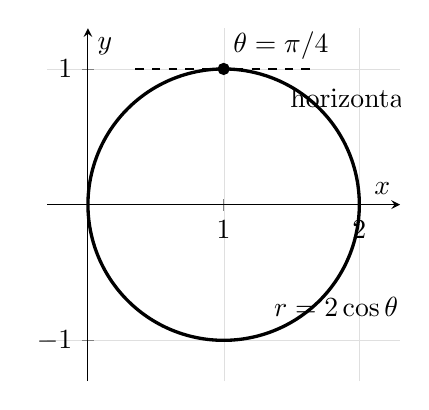
\begin{tikzpicture}
\begin{axis}[
    width=0.62\textwidth,
    height=0.50\textwidth,
    xmin=-0.3, xmax=2.3,
    ymin=-1.3, ymax=1.3,
    axis lines=middle,
    xlabel={\(x\)},
    ylabel={\(y\)},
    xtick={0,1,2},
    ytick={-1,0,1},
    axis equal image,
    grid=both,
    grid style={line width=.1pt, draw=gray!25},
]
\addplot[very thick, domain=-1.5707963:1.5707963, samples=240]
    ({2*cos(deg(x))*cos(deg(x))},{2*cos(deg(x))*sin(deg(x))});

\addplot[only marks, mark=*] coordinates {(1,1)};
\addplot[thick, dashed, domain=0.35:1.65, samples=2] {1};

\node[anchor=south west] at (axis cs:1,1) {\(\theta=\pi/4\)};
\node[anchor=west] at (axis cs:1.42,0.77) {horizontal tangent};
\node[anchor=west] at (axis cs:1.3,-0.75) {\(r=2\cos\theta\)};
\end{axis}
\end{tikzpicture}
\caption{The polar slope formula gives a horizontal tangent at the top of the circle \(r=2\cos\theta\).}
\label{fig:polar-circle-slope}
\end{figure}

\paragraph{Horizontal and vertical tangents.}
The polar slope formula also tells us when tangents are horizontal or vertical.

A horizontal tangent occurs when

\[
\frac{dy}{d\theta}=0
\]

and

\[
\frac{dx}{d\theta}\neq0.
\]

So for a polar curve,

\[
\boxed{
r'(\theta)\sin\theta+r(\theta)\cos\theta=0
}
\]

with

\[
r'(\theta)\cos\theta-r(\theta)\sin\theta\neq0.
\]

A vertical tangent occurs when

\[
\frac{dx}{d\theta}=0
\]

and

\[
\frac{dy}{d\theta}\neq0.
\]

So

\[
\boxed{
r'(\theta)\cos\theta-r(\theta)\sin\theta=0
}
\]

with

\[
r'(\theta)\sin\theta+r(\theta)\cos\theta\neq0.
\]

\begin{quote}
\textbf{Warning.}
If both

\[
\frac{dx}{d\theta}=0
\qquad\text{and}\qquad
\frac{dy}{d\theta}=0,
\]

then the quotient gives \(0/0\).  The tangent is not decided by direct substitution.
Study the nearby motion.
\end{quote}

This warning is especially important at cusps.

For the cardioid

\[
r=1+\cos\theta,
\]

the point \(\theta=\pi\) gives

\[
r=0,
\qquad
r'=-\sin\pi=0.
\]

Thus

\[
x'(\pi)=0,
\qquad
y'(\pi)=0.
\]

The moving point has stopped at the origin.  The curve still has a tangent there, but the
simple slope formula cannot find it by direct substitution.

\subsection{Area in polar coordinates}
\label{subsec:area-polar-coordinates}

The ordinary area formula for a graph uses vertical strips:

\[
dA=y\,dx.
\]

A polar graph suggests a different small piece.  When \(\theta\) changes by a small amount
\(\Delta\theta\), the radius sweeps out a thin sector.

For a circle of radius \(r\), a sector with angle \(\Delta\theta\) has area

\[
\frac12 r^2\Delta\theta.
\]

For a polar curve \(r=f(\theta)\), if \(\Delta\theta\) is small, the radius is nearly constant
on that small angular interval.  So the small sector area is approximately

\[
\Delta A\approx \frac12 r^2\Delta\theta.
\]

Adding these small sectors gives the polar area formula.

\begin{quote}
\textbf{Area in polar coordinates.}
If the polar curve

\[
r=f(\theta),
\qquad
\alpha\le\theta\le\beta,
\]

traces a region once, then the area swept out by the radius vector is

\[
\boxed{
A=\frac12\int_\alpha^\beta \bigl(f(\theta)\bigr)^2\,d\theta.
}
\]
\end{quote}

This formula is easy to remember:

\[
\boxed{
dA=\frac12r^2\,d\theta.
}
\]

It is the small area of a thin sector.

\begin{figure}[h]
\centering
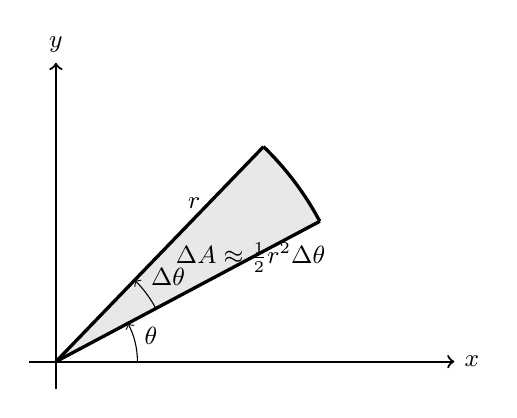
\begin{tikzpicture}[scale=1.15, every node/.style={font=\small}]
  % axes
  \draw[->, thick] (-0.3,0) -- (4.4,0) node[right] {\(x\)};
  \draw[->, thick] (0,-0.3) -- (0,3.3) node[above] {\(y\)};

  % angles
  \def\a{28}
  \def\b{46}
  \def\rA{3.3}
  \def\rB{3.3}

  % sector
  \fill[gray!18] (0,0) -- ({\rA*cos(\a)},{\rA*sin(\a)})
    arc (\a:\b:\rA) -- cycle;
  \draw[very thick] (0,0) -- ({\rA*cos(\a)},{\rA*sin(\a)});
  \draw[very thick] (0,0) -- ({\rA*cos(\b)},{\rA*sin(\b)});
  \draw[very thick] ({\rA*cos(\a)},{\rA*sin(\a)})
    arc (\a:\b:\rA);

  % angle arcs
  \draw[->] (0.9,0) arc (0:\a:0.9);
  \node at (1.05,0.28) {\(\theta\)};
  \draw[->] ({1.25*cos(\a)},{1.25*sin(\a)})
    arc (\a:\b:1.25);
  \node at ({1.55*cos(37)},{1.55*sin(37)}) {\(\Delta\theta\)};

  \node[above] at ({2.2*cos(\b)},{2.2*sin(\b)}) {\(r\)};
  \node at (2.15,1.15) {\(\Delta A\approx \frac12 r^2\Delta\theta\)};
\end{tikzpicture}
\caption{A small angular slice is approximately a sector of area \(\frac12r^2\Delta\theta\).}
\label{fig:polar-sector-area}
\end{figure}

There is also a parametric reason for the same formula.  For a closed curve traced
counterclockwise,

\[
A=\frac12\int (x y'-y x')\,d\theta.
\]

With

\[
x=r\cos\theta,
\qquad
y=r\sin\theta,
\]

we have

\[
x y'-y x'=r^2.
\]

So

\[
A=\frac12\int r^2\,d\theta.
\]

The sector picture and the parametric area formula agree.

\paragraph{Example: area of a circle.}
The polar equation

\[
r=R
\]

traces a circle of radius \(R\) centered at the origin when

\[
0\le\theta\le2\pi.
\]

The polar area formula gives

\[
A=\frac12\int_0^{2\pi}R^2\,d\theta.
\]

Thus

\[
A=\frac12R^2(2\pi)=\boxed{\pi R^2}.
\]

The familiar circle area formula is a sector accumulation.

\paragraph{Example: area inside a cardioid.}
Find the area enclosed by

\[
r=1+\cos\theta.
\]

The cardioid is traced once for

\[
0\le\theta\le2\pi.
\]

So

\[
A=\frac12\int_0^{2\pi}(1+\cos\theta)^2\,d\theta.
\]

Expand:

\[
(1+\cos\theta)^2=1+2\cos\theta+\cos^2\theta.
\]

Therefore

\[
A
=
\frac12\int_0^{2\pi}
\left(1+2\cos\theta+\cos^2\theta\right)\,d\theta.
\]

Now

\[
\int_0^{2\pi}1\,d\theta=2\pi,
\]

\[
\int_0^{2\pi}\cos\theta\,d\theta=0,
\]

and

\[
\int_0^{2\pi}\cos^2\theta\,d\theta=\pi.
\]

Thus

\[
A=\frac12(2\pi+\pi)=\boxed{\frac{3\pi}{2}}.
\]

\begin{figure}[h]
\centering
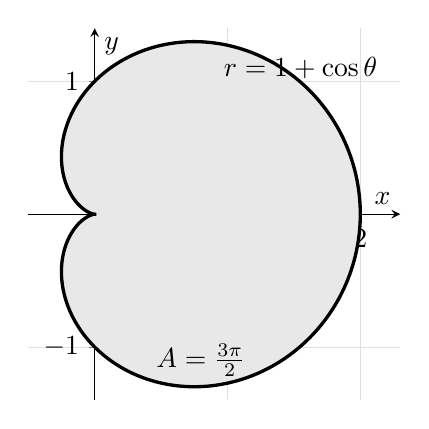
\begin{tikzpicture}
\begin{axis}[
    width=0.66\textwidth,
    height=0.52\textwidth,
    xmin=-0.5, xmax=2.3,
    ymin=-1.4, ymax=1.4,
    axis lines=middle,
    xlabel={\(x\)},
    ylabel={\(y\)},
    xtick={0,1,2},
    ytick={-1,0,1},
    axis equal image,
    grid=both,
    grid style={line width=.1pt, draw=gray!25},
]
\addplot[domain=0:6.283185, samples=400, fill=gray!18, draw=none]
    ({(1+cos(deg(x)))*cos(deg(x))},{(1+cos(deg(x)))*sin(deg(x))}) \closedcycle;
\addplot[very thick, domain=0:6.283185, samples=400]
    ({(1+cos(deg(x)))*cos(deg(x))},{(1+cos(deg(x)))*sin(deg(x))});
\node[anchor=west] at (axis cs:0.9,1.1) {\(r=1+\cos\theta\)};
\node at (axis cs:0.8,-1.1) {\(A=\frac{3\pi}{2}\)};
\end{axis}
\end{tikzpicture}
\caption{The cardioid area is found by accumulating small sectors.}
\label{fig:cardioid-area-polar}
\end{figure}

\paragraph{Area between two polar curves.}
If two polar curves share the same angular interval and one lies outside the other, then
we subtract sector areas.

Suppose

\[
r=R(\theta)
\]

is the outer curve and

\[
r=\rho(\theta)
\]

is the inner curve on

\[
\alpha\le\theta\le\beta.
\]

Then

\[
\boxed{
A=\frac12\int_\alpha^\beta
\left(R(\theta)^2-\rho(\theta)^2\right)\,d\theta.
}
\]

In words,

\[
\boxed{
\text{polar area between curves}
=
\frac12\int
\left((\text{outer radius})^2-(\text{inner radius})^2\right)\,d\theta.
}
\]

The square is not optional.  Sector area depends on \(r^2\), not on \(r\).

\paragraph{Example: one petal of a rose.}
Find the area of one petal of

\[
r=2\cos(3\theta).
\]

One petal is traced while \(r\ge0\) around \(\theta=0\).  The zeros occur when

\[
2\cos(3\theta)=0,
\]

so

\[
3\theta=\pm\frac{\pi}{2}.
\]

Thus one petal is traced for

\[
-\frac{\pi}{6}\le\theta\le\frac{\pi}{6}.
\]

The area is

\[
A=\frac12\int_{-\pi/6}^{\pi/6}4\cos^2(3\theta)\,d\theta.
\]

So

\[
A=2\int_{-\pi/6}^{\pi/6}\cos^2(3\theta)\,d\theta.
\]

Let

\[
u=3\theta,
\qquad
du=3\,d\theta.
\]

Then

\[
A=\frac23\int_{-\pi/2}^{\pi/2}\cos^2 u\,du.
\]

Since

\[
\int_{-\pi/2}^{\pi/2}\cos^2u\,du=\frac{\pi}{2},
\]

we get

\[
\boxed{
A=\frac{\pi}{3}.
}
\]

The whole rose has three petals, so its total area is

\[
\pi.
\]

\begin{quote}
\textbf{Warning.}
Before using

\[
A=\frac12\int r^2\,d\theta,
\]

check what interval traces the region exactly once.  Polar curves can retrace themselves,
and negative \(r\) can send points to the opposite side of the origin.
\end{quote}

\subsection{Arc length in polar coordinates}
\label{subsec:arc-length-polar-coordinates}

A polar curve is parametric:

\[
x=r\cos\theta,
\qquad
y=r\sin\theta.
\]

So its length is

\[
L=\int_\alpha^\beta
\sqrt{\left(\frac{dx}{d\theta}\right)^2+
      \left(\frac{dy}{d\theta}\right)^2}\,d\theta.
\]

We already computed

\[
\frac{dx}{d\theta}
=
r'\cos\theta-r\sin\theta,
\]

and

\[
\frac{dy}{d\theta}
=
r'\sin\theta+r\cos\theta.
\]

Now square and add:

\[
\left(r'\cos\theta-r\sin\theta\right)^2
+
\left(r'\sin\theta+r\cos\theta\right)^2.
\]

Expand:

\[
(r')^2\cos^2\theta-2rr'\sin\theta\cos\theta+r^2\sin^2\theta
\]

\[
+
(r')^2\sin^2\theta+2rr'\sin\theta\cos\theta+r^2\cos^2\theta.
\]

The cross terms cancel.  The remaining terms give

\[
(r')^2(\cos^2\theta+\sin^2\theta)
+
r^2(\sin^2\theta+\cos^2\theta).
\]

So the square of the speed is

\[
(r')^2+r^2.
\]

Therefore

\[
\boxed{
L=\int_\alpha^\beta
\sqrt{\left(\frac{dr}{d\theta}\right)^2+r^2}\,d\theta.
}
\]

\begin{quote}
\textbf{Arc length in polar coordinates.}
For

\[
r=r(\theta),
\qquad
\alpha\le\theta\le\beta,
\]

the length of the polar curve is

\[
\boxed{
L=\int_\alpha^\beta
\sqrt{r(\theta)^2+\bigl(r'(\theta)\bigr)^2}\,d\theta.
}
\]
\end{quote}

The formula has a nice geometric meaning.  As \(\theta\) changes, the point may move
radially because \(r\) changes, and it may move around the origin because the angle
changes.  The two effects combine by the Pythagorean theorem.

\paragraph{Example: circumference of a circle.}
For

\[
r=R,
\]

we have

\[
r'=0.
\]

Thus

\[
L=\int_0^{2\pi}\sqrt{R^2+0^2}\,d\theta
=
\int_0^{2\pi}R\,d\theta
=
\boxed{2\pi R}.
\]

\paragraph{Example: length of a cardioid.}
Find the length of

\[
r=1+\cos\theta,
\qquad
0\le\theta\le2\pi.
\]

We have

\[
r'=-\sin\theta.
\]

So

\[
r^2+(r')^2
=
(1+\cos\theta)^2+\sin^2\theta.
\]

Expand and simplify:

\[
(1+\cos\theta)^2+\sin^2\theta
=
1+2\cos\theta+\cos^2\theta+\sin^2\theta
=
2+2\cos\theta.
\]

Using

\[
1+\cos\theta=2\cos^2\left(\frac{\theta}{2}\right),
\]

we get

\[
2+2\cos\theta
=
4\cos^2\left(\frac{\theta}{2}\right).
\]

Therefore

\[
\sqrt{r^2+(r')^2}
=
2\left|\cos\left(\frac{\theta}{2}\right)\right|.
\]

So

\[
L=\int_0^{2\pi}
2\left|\cos\left(\frac{\theta}{2}\right)\right|\,d\theta.
\]

On \(0\le\theta\le\pi\), \(\cos(\theta/2)\ge0\).  On \(\pi\le\theta\le2\pi\), it is
nonpositive.  Therefore

\[
L=
\int_0^\pi 2\cos\left(\frac{\theta}{2}\right)\,d\theta
+
\int_\pi^{2\pi} -2\cos\left(\frac{\theta}{2}\right)\,d\theta.
\]

Compute:

\[
\int 2\cos\left(\frac{\theta}{2}\right)\,d\theta
=
4\sin\left(\frac{\theta}{2}\right).
\]

Thus the first integral is

\[
4\sin\left(\frac{\pi}{2}\right)-4\sin0=4.
\]

The second integral is

\[
-4\sin\left(\frac{\theta}{2}\right)\Big|_\pi^{2\pi}
=
-4\sin\pi+4\sin\left(\frac{\pi}{2}\right)
=
4.
\]

So

\[
\boxed{
L=8.
}
\]

\begin{quote}
\textbf{A small absolute value warning.}
The expression

\[
\sqrt{4\cos^2(\theta/2)}
\]

equals

\[
2|\cos(\theta/2)|,
\]

not always \(2\cos(\theta/2)\).  Dropping the absolute value would incorrectly make
the length cancel to zero.
\end{quote}

\subsection{Intersections and repeated tracing}
\label{subsec:polar-intersections-repeated-tracing}

Polar coordinates are not unique.  That nonuniqueness is useful, but it makes
intersections more delicate than in Cartesian coordinates.

Two polar curves can meet even when their equations do not give the same \(r\) at the
same \(\theta\).

There are three common issues.

\begin{center}
\begin{tabular}{c|p{0.62\textwidth}}
\textbf{Issue} & \textbf{What to check} \\ \hline
Same ray intersections & Solve \(r_1(\theta)=r_2(\theta)\). \\[3pt]
The origin & Check whether each curve reaches \(r=0\), possibly at different angles. \\[3pt]
Negative \(r\) and alternate angles & Remember \((r,\theta)=(-r,\theta+\pi)\).
\end{tabular}
\end{center}

\paragraph{Example: an intersection missed by the same-angle equation.}
Consider

\[
r=2\cos\theta
\]

and

\[
r=2\sin\theta.
\]

These are two circles:

\[
(x-1)^2+y^2=1
\]

and

\[
x^2+(y-1)^2=1.
\]

Solving with the same angle gives

\[
2\cos\theta=2\sin\theta.
\]

So

\[
\cos\theta=\sin\theta,
\]

and hence

\[
\theta=\frac{\pi}{4}.
\]

At this angle,

\[
r=\sqrt2,
\]

so the point is

\[
(1,1).
\]

But the circles also meet at the origin.

Why did the same-angle equation miss it?

For

\[
r=2\cos\theta,
\]

the origin occurs when

\[
\cos\theta=0,
\]

for example at

\[
\theta=\frac{\pi}{2}.
\]

For

\[
r=2\sin\theta,
\]

the origin occurs when

\[
\sin\theta=0,
\]

for example at

\[
\theta=0.
\]

The two curves reach the same Cartesian point with different polar angles.  Therefore
the same-angle equation did not see that intersection.

\begin{figure}[h]
\centering
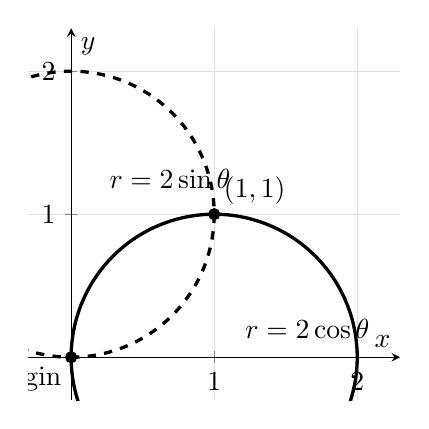
\begin{tikzpicture}
\begin{axis}[
    width=0.62\textwidth,
    height=0.52\textwidth,
    xmin=-0.3, xmax=2.3,
    ymin=-0.3, ymax=2.3,
    axis lines=middle,
    xlabel={\(x\)},
    ylabel={\(y\)},
    xtick={0,1,2},
    ytick={0,1,2},
    axis equal image,
    grid=both,
    grid style={line width=.1pt, draw=gray!25},
]
\addplot[very thick, domain=-1.5707963:1.5707963, samples=240]
    ({2*cos(deg(x))*cos(deg(x))},{2*cos(deg(x))*sin(deg(x))});
\addplot[very thick, dashed, domain=0:3.1415926, samples=240]
    ({2*sin(deg(x))*cos(deg(x))},{2*sin(deg(x))*sin(deg(x))});

\addplot[only marks, mark=*] coordinates {(0,0) (1,1)};
\node[anchor=north east] at (axis cs:0,0) {origin};
\node[anchor=south west] at (axis cs:1,1) {\((1,1)\)};
\node[anchor=west] at (axis cs:1.15,0.2) {\(r=2\cos\theta\)};
\node[anchor=west] at (axis cs:0.2,1.25) {\(r=2\sin\theta\)};
\end{axis}
\end{tikzpicture}
\caption{The two circles intersect at \((1,1)\) and at the origin.  The origin is reached at different polar angles.}
\label{fig:polar-intersections-origin}
\end{figure}

\paragraph{Repeated tracing.}
Polar curves can also trace the same geometric curve more than once.

For example,

\[
r=2\cos\theta
\]

is one circle.  The interval

\[
-\frac{\pi}{2}\le\theta\le\frac{\pi}{2}
\]

traces it once.

But the interval

\[
0\le\theta\le2\pi
\]

traces the same circle twice.

If we blindly use the polar area formula on \(0\le\theta\le2\pi\), we get

\[
A=\frac12\int_0^{2\pi}(2\cos\theta)^2\,d\theta.
\]

This becomes

\[
A=2\int_0^{2\pi}\cos^2\theta\,d\theta
=
2\pi.
\]

But the circle has radius \(1\), so its area is only

\[
\pi.
\]

The integral doubled the answer because the parametrization traced the circle twice.

Using the once-around interval gives

\[
A=\frac12\int_{-\pi/2}^{\pi/2}(2\cos\theta)^2\,d\theta.
\]

So

\[
A=2\int_{-\pi/2}^{\pi/2}\cos^2\theta\,d\theta
=
2\cdot\frac{\pi}{2}
=
\pi.
\]

That is correct.

\begin{quote}
\textbf{Polar checklist before computing area or length.}

Before using a polar formula, ask:

\begin{enumerate}
\item What interval of \(\theta\) traces the desired curve?

\item Is the curve traced once or more than once?

\item Does \(r\) become negative, creating points on the opposite ray?

\item Does the curve pass through the origin?

\item If two curves intersect, are there intersections reached at different angles?
\end{enumerate}
\end{quote}

Polar coordinates are powerful because they match circular and radial geometry.  But
the price is that the same point may have many names.

The next family of curves makes especially good use of polar coordinates.  It includes
parabolas, ellipses, and hyperbolas.  These curves can be described by distance from a
fixed point and a fixed line, and in polar form they appear in one equation.

\section{Conic sections}
\label{sec:conic-sections}

Circles, parabolas, ellipses, and hyperbolas look like different curves.  But they belong
to one family.

One way to discover them is to slice a cone.  A horizontal slice gives a circle.  A slanted
slice may give an ellipse, a parabola, or a hyperbola.

There is another way, better suited to calculus and polar coordinates: compare distances.

A conic is controlled by a fixed point and a fixed line.

\[
\text{fixed point: focus}
\qquad
\text{fixed line: directrix}
\]

The curve consists of all points whose distance to the focus has a constant ratio to their
distance to the directrix.

That ratio is called the eccentricity.

\subsection{Parabolas, ellipses, and hyperbolas from focus and directrix}
\label{subsec:conics-focus-directrix}

Start with the most familiar focus-directrix example.

Let the focus be

\[
F=(0,p),
\qquad p>0,
\]

and let the directrix be the horizontal line

\[
y=-p.
\]

A point \(P=(x,y)\) is on the parabola if its distance to the focus equals its distance to
the directrix.

The distance from \(P=(x,y)\) to the focus \(F=(0,p)\) is

\[
\sqrt{x^2+(y-p)^2}.
\]

The distance from \(P=(x,y)\) to the directrix \(y=-p\) is

\[
y+p
\]

for points above the directrix.

Set the distances equal:

\[
\sqrt{x^2+(y-p)^2}=y+p.
\]

Square both sides:

\[
x^2+(y-p)^2=(y+p)^2.
\]

Expand:

\[
x^2+y^2-2py+p^2=y^2+2py+p^2.
\]

Cancel \(y^2\) and \(p^2\):

\[
x^2-2py=2py.
\]

So

\[
\boxed{
x^2=4py.
}
\]

This is the standard upward-opening parabola with vertex at the origin.

\begin{figure}[h]
\centering
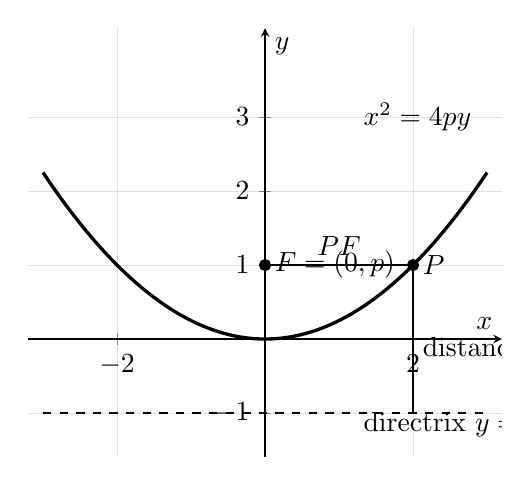
\begin{tikzpicture}
\begin{axis}[
    width=0.66\textwidth,
    height=0.58\textwidth,
    xmin=-3.2, xmax=3.2,
    ymin=-1.6, ymax=4.2,
    axis lines=middle,
    xlabel={\(x\)},
    ylabel={\(y\)},
    xtick={-2,0,2},
    ytick={-1,0,1,2,3},
    axis equal image,
    grid=both,
    grid style={line width=.1pt, draw=gray!25},
]
% p=1, parabola x^2=4y -> y=x^2/4
\addplot[very thick, domain=-3:3, samples=160] {x^2/4};

% directrix
\addplot[thick, dashed, domain=-3:3, samples=2] {-1};

% focus
\addplot[only marks, mark=*] coordinates {(0,1)};
\node[anchor=west] at (axis cs:0,1) {\(F=(0,p)\)};

% sample point x=2, y=1
\addplot[only marks, mark=*] coordinates {(2,1)};
\node[anchor=west] at (axis cs:2,1) {\(P\)};

% distance to focus and directrix
\draw[thick] (axis cs:2,1) -- (axis cs:0,1);
\draw[thick] (axis cs:2,1) -- (axis cs:2,-1);
\node[anchor=south] at (axis cs:1,1) {\(PF\)};
\node[anchor=west] at (axis cs:2,-0.1) {distance to directrix};

\node[anchor=west] at (axis cs:1.2,-1.15) {directrix \(y=-p\)};
\node[anchor=west] at (axis cs:1.2,3.0) {\(x^2=4py\)};
\end{axis}
\end{tikzpicture}
\caption{A parabola is the set of points equidistant from a focus and a directrix.}
\label{fig:parabola-focus-directrix}
\end{figure}

The parabola is only one member of the family.  To get the whole family, allow a constant
ratio.

\begin{quote}
\textbf{Focus-directrix definition of a conic.}
Fix a point \(F\), called the \emph{focus}, and a line \(\ell\), called the \emph{directrix}.
For a positive number \(e\), the conic with eccentricity \(e\) is the set of points \(P\)
such that

\[
\boxed{
\operatorname{dist}(P,F)=e\,\operatorname{dist}(P,\ell).
}
\]

The number \(e\) is called the \emph{eccentricity}.
\end{quote}

The value of \(e\) determines the kind of conic.

\begin{center}
\begin{tabular}{c|c}
\textbf{eccentricity} & \textbf{type of conic} \\ \hline
\(0<e<1\) & ellipse \\
\(e=1\) & parabola \\
\(e>1\) & hyperbola
\end{tabular}
\end{center}

A circle is the perfectly symmetric special case of an ellipse.  In the usual two-focus
description of ellipses, a circle has eccentricity \(e=0\).  The focus-directrix description
above is most useful for \(e>0\).

\paragraph{Why the ratio matters.}
If

\[
e=1,
\]

then the point is equally far from the focus and the directrix.  This gives a parabola.

If

\[
0<e<1,
\]

then

\[
\operatorname{dist}(P,F)<\operatorname{dist}(P,\ell).
\]

The focus distance is smaller than the directrix distance.  The resulting curve closes up
into an ellipse.

If

\[
e>1,
\]

then

\[
\operatorname{dist}(P,F)>\operatorname{dist}(P,\ell).
\]

The focus distance is larger than the directrix distance.  The resulting curve opens into
a hyperbola.

\subsection{Standard equations}
\label{subsec:standard-equations-conics}

The focus-directrix definition gives the geometry.  The standard equations give the
algebra.

\subsubsection*{Parabolas}

We already derived

\[
\boxed{
x^2=4py.
}
\]

This parabola has

\[
\text{vertex }(0,0),
\qquad
\text{focus }(0,p),
\qquad
\text{directrix }y=-p.
\]

It opens upward when \(p>0\) and downward when \(p<0\).

The sideways form is

\[
\boxed{
y^2=4px.
}
\]

This parabola has

\[
\text{focus }(p,0),
\qquad
\text{directrix }x=-p.
\]

It opens right when \(p>0\) and left when \(p<0\).

\paragraph{Example.}
Find the focus and directrix of

\[
y^2=12x.
\]

Compare with

\[
y^2=4px.
\]

So

\[
4p=12,
\qquad
p=3.
\]

Therefore the focus is

\[
(3,0),
\]

and the directrix is

\[
x=-3.
\]

\subsubsection*{Ellipses}

An ellipse can be described as the set of points whose distances to two fixed foci have
constant sum.

For the horizontal ellipse centered at the origin,

\[
\boxed{
\frac{x^2}{a^2}+\frac{y^2}{b^2}=1,
\qquad
a\ge b>0.
}
\]

The longer axis is along the \(x\)-axis.  The vertices are

\[
(\pm a,0),
\]

and the endpoints of the shorter axis are

\[
(0,\pm b).
\]

The foci are

\[
(\pm c,0),
\]

where

\[
\boxed{
c^2=a^2-b^2.
}
\]

The eccentricity is

\[
\boxed{
e=\frac{c}{a}.
}
\]

Because \(c<a\), an ellipse has

\[
0\le e<1.
\]

If \(a=b\), then \(c=0\), the two foci coincide at the center, and the ellipse is a circle.

\paragraph{Example.}
Find the foci and eccentricity of

\[
\frac{x^2}{25}+\frac{y^2}{9}=1.
\]

Here

\[
a^2=25,
\qquad
b^2=9.
\]

So

\[
a=5,
\qquad
b=3.
\]

Then

\[
c^2=a^2-b^2=25-9=16,
\]

so

\[
c=4.
\]

The foci are

\[
(\pm4,0).
\]

The eccentricity is

\[
e=\frac{c}{a}=\frac45.
\]

\subsubsection*{Hyperbolas}

A hyperbola can be described as the set of points whose distances to two fixed foci have
constant difference.

For the horizontal hyperbola centered at the origin,

\[
\boxed{
\frac{x^2}{a^2}-\frac{y^2}{b^2}=1.
}
\]

The vertices are

\[
(\pm a,0).
\]

The foci are

\[
(\pm c,0),
\]

where

\[
\boxed{
c^2=a^2+b^2.
}
\]

The eccentricity is

\[
\boxed{
e=\frac{c}{a}.
}
\]

Because \(c>a\), a hyperbola has

\[
e>1.
\]

The asymptotes are

\[
\boxed{
y=\pm\frac{b}{a}x.
}
\]

\paragraph{Example.}
Find the foci and asymptotes of

\[
\frac{x^2}{9}-\frac{y^2}{16}=1.
\]

Here

\[
a^2=9,
\qquad
b^2=16,
\]

so

\[
a=3,
\qquad
b=4.
\]

For a hyperbola,

\[
c^2=a^2+b^2=9+16=25,
\]

so

\[
c=5.
\]

The foci are

\[
(\pm5,0).
\]

The asymptotes are

\[
y=\pm\frac{4}{3}x.
\]

The eccentricity is

\[
e=\frac{c}{a}=\frac53.
\]

\begin{center}
\begin{tabular}{c|c|c|c}
\textbf{conic} & \textbf{standard equation} & \textbf{focal relation} & \textbf{eccentricity} \\ \hline
parabola & \(x^2=4py\) & one focus and one directrix & \(e=1\) \\[3pt]
ellipse & \(\dfrac{x^2}{a^2}+\dfrac{y^2}{b^2}=1\) & \(c^2=a^2-b^2\) & \(0\le e<1\) \\[8pt]
hyperbola & \(\dfrac{x^2}{a^2}-\dfrac{y^2}{b^2}=1\) & \(c^2=a^2+b^2\) & \(e>1\)
\end{tabular}
\end{center}

\begin{figure}[h]
\centering
\begin{minipage}{0.47\textwidth}
\centering
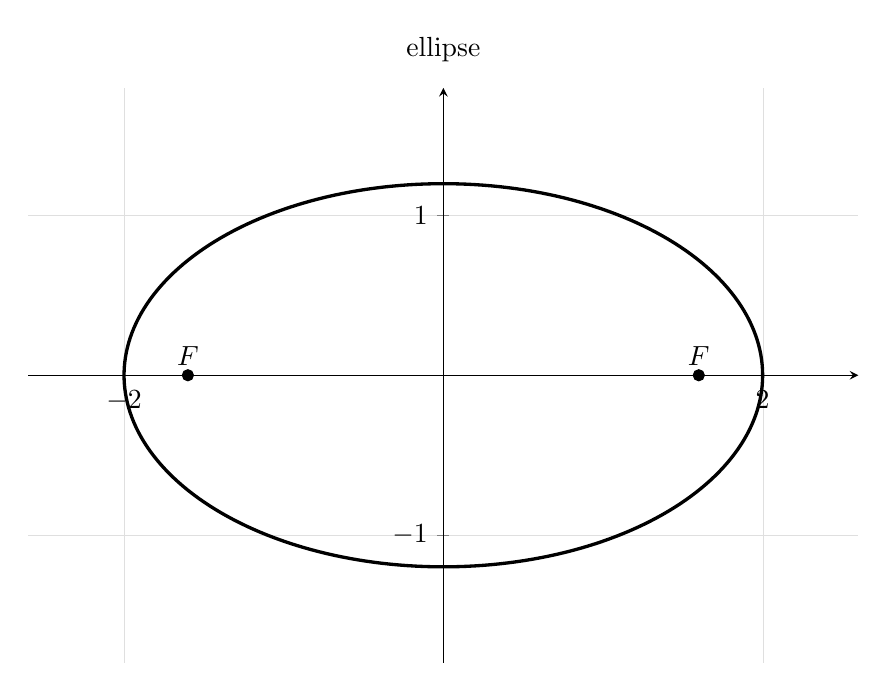
\begin{tikzpicture}
\begin{axis}[
    width=\textwidth,
    height=0.80\textwidth,
    xmin=-2.6, xmax=2.6,
    ymin=-1.8, ymax=1.8,
    axis lines=middle,
    xtick={-2,0,2},
    ytick={-1,0,1},
    axis equal image,
    grid=both,
    grid style={line width=.1pt, draw=gray!25},
    title={ellipse}
]
\addplot[very thick, domain=0:360, samples=240]
    ({2*cos(x)},{1.2*sin(x)});
\addplot[only marks, mark=*] coordinates {(-1.6,0) (1.6,0)};
\node[anchor=south] at (axis cs:-1.6,0) {\(F\)};
\node[anchor=south] at (axis cs:1.6,0) {\(F\)};
\end{axis}
\end{tikzpicture}
\end{minipage}
\hfill
\begin{minipage}{0.47\textwidth}
\centering
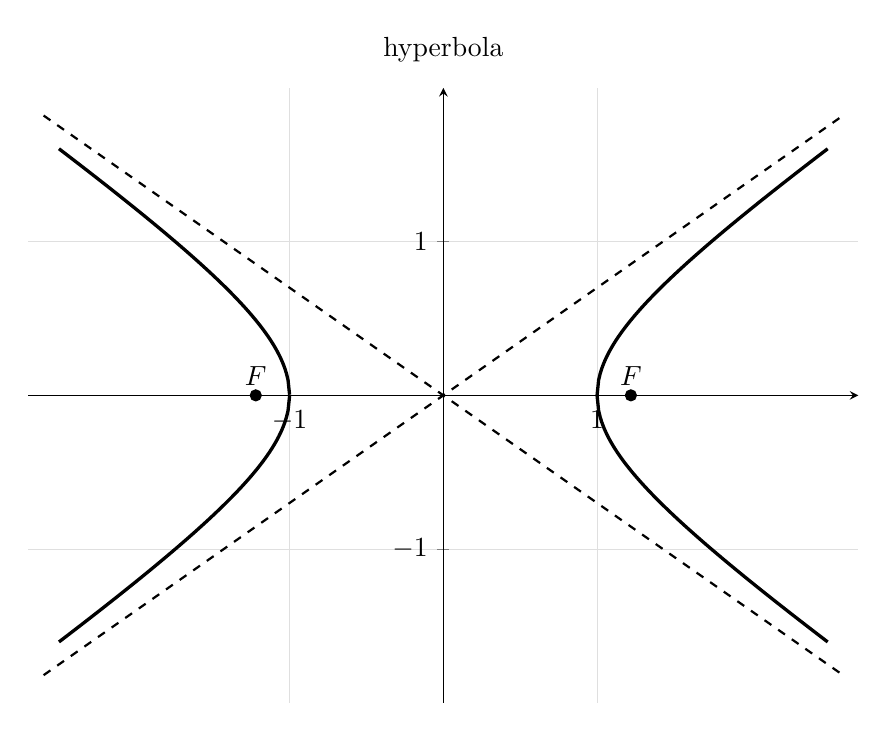
\begin{tikzpicture}
\begin{axis}[
    width=\textwidth,
    height=0.80\textwidth,
    xmin=-2.7, xmax=2.7,
    ymin=-2.0, ymax=2.0,
    axis lines=middle,
    xtick={-1,0,1},
    ytick={-1,0,1},
    axis equal image,
    grid=both,
    grid style={line width=.1pt, draw=gray!25},
    title={hyperbola}
]
\addplot[very thick, domain=1:2.5, samples=150] {0.7*sqrt(x^2-1)};
\addplot[very thick, domain=1:2.5, samples=150] {-0.7*sqrt(x^2-1)};
\addplot[very thick, domain=-2.5:-1, samples=150] {0.7*sqrt(x^2-1)};
\addplot[very thick, domain=-2.5:-1, samples=150] {-0.7*sqrt(x^2-1)};
\addplot[thick, dashed, domain=-2.6:2.6, samples=2] {0.7*x};
\addplot[thick, dashed, domain=-2.6:2.6, samples=2] {-0.7*x};
\addplot[only marks, mark=*] coordinates {(-1.22,0) (1.22,0)};
\node[anchor=south] at (axis cs:-1.22,0) {\(F\)};
\node[anchor=south] at (axis cs:1.22,0) {\(F\)};
\end{axis}
\end{tikzpicture}
\end{minipage}
\caption{Ellipses close up because \(0\le e<1\).  Hyperbolas open because \(e>1\).}
\label{fig:ellipse-hyperbola-standard}
\end{figure}

\subsection{Polar equations of conics}
\label{subsec:polar-equations-conics}

The focus-directrix definition becomes especially simple in polar coordinates if we place
the focus at the origin.

Let the focus be the pole.  Let the directrix be the vertical line

\[
x=d,
\qquad d>0.
\]

For a point \(P\) with polar coordinates \((r,\theta)\), the distance to the focus is

\[
r.
\]

The Cartesian \(x\)-coordinate of \(P\) is

\[
x=r\cos\theta.
\]

So the distance from \(P\) to the directrix \(x=d\), for points to the left of the directrix,
is

\[
d-r\cos\theta.
\]

The focus-directrix condition is

\[
r=e(d-r\cos\theta).
\]

Solve for \(r\):

\[
r=ed-er\cos\theta.
\]

Move the \(r\)-terms together:

\[
r+er\cos\theta=ed.
\]

Factor:

\[
r(1+e\cos\theta)=ed.
\]

Therefore

\[
r=\frac{ed}{1+e\cos\theta}.
\]

If we write

\[
p=ed,
\]

then

\[
\boxed{
r=\frac{p}{1+e\cos\theta}.
}
\]

The number \(p\) is called the \emph{semi-latus rectum}.  It is the radius when

\[
\theta=\frac{\pi}{2}
\]

or

\[
\theta=\frac{3\pi}{2},
\]

provided those points are on the curve.

Changing the position of the directrix changes the sign or replaces cosine by sine.  The
common polar forms are

\[
\boxed{
r=\frac{p}{1\pm e\cos\theta}
}
\]

and

\[
\boxed{
r=\frac{p}{1\pm e\sin\theta}.
}
\]

The same eccentricity test applies:

\begin{center}
\begin{tabular}{c|c}
\textbf{eccentricity in polar equation} & \textbf{conic} \\ \hline
\(0<e<1\) & ellipse \\
\(e=1\) & parabola \\
\(e>1\) & hyperbola
\end{tabular}
\end{center}

\paragraph{Example: identify a polar conic.}
Classify

\[
r=\frac{6}{2+\cos\theta}.
\]

First rewrite the denominator so that it has the form \(1+e\cos\theta\):

\[
r
=
\frac{6}{2+\cos\theta}
=
\frac{3}{1+\frac12\cos\theta}.
\]

Thus

\[
p=3,
\qquad
e=\frac12.
\]

Since

\[
0<e<1,
\]

the conic is an ellipse.

\paragraph{Example: a parabola in polar form.}
Consider

\[
r=\frac{4}{1+\cos\theta}.
\]

Here

\[
e=1,
\]

so the curve is a parabola.

We can also convert it to Cartesian form.  Multiply both sides by the denominator:

\[
r(1+\cos\theta)=4.
\]

Since

\[
r\cos\theta=x,
\]

this becomes

\[
r+x=4.
\]

Thus

\[
r=4-x.
\]

Now use

\[
r=\sqrt{x^2+y^2}.
\]

So

\[
\sqrt{x^2+y^2}=4-x.
\]

Square both sides:

\[
x^2+y^2=(4-x)^2.
\]

Expand:

\[
x^2+y^2=16-8x+x^2.
\]

Cancel \(x^2\):

\[
y^2=16-8x.
\]

So

\[
\boxed{
y^2=-8(x-2).
}
\]

This is a parabola opening left.  Its focus is at the origin, exactly as the polar setup
promised.

\begin{figure}[h]
\centering
\begin{tikzpicture}
\begin{axis}[
    width=0.70\textwidth,
    height=0.54\textwidth,
    xmin=-4.0, xmax=2.5,
    ymin=-4.0, ymax=4.0,
    axis lines=middle,
    xlabel={\(x\)},
    ylabel={\(y\)},
    xtick={-4,-2,0,2},
    ytick={-4,-2,0,2,4},
    axis equal image,
    grid=both,
    grid style={line width=.1pt, draw=gray!25},
]
\addplot[very thick, domain=-2.75:2.75, samples=250]
    ({(4/(1+cos(deg(x))))*cos(deg(x))},
     {(4/(1+cos(deg(x))))*sin(deg(x))});

\addplot[only marks, mark=*] coordinates {(0,0) (2,0)};
\node[anchor=south east] at (axis cs:0,0) {focus};
\node[anchor=south] at (axis cs:2,0) {vertex};
\node[anchor=west] at (axis cs:-3.4,2.8) {\(r=\dfrac{4}{1+\cos\theta}\)};
\node[anchor=west] at (axis cs:-3.4,2.2) {\(y^2=-8(x-2)\)};
\end{axis}
\end{tikzpicture}
\caption{The polar equation \(r=\frac{4}{1+\cos\theta}\) is a parabola with focus at the pole.}
\label{fig:polar-parabola-conic}
\end{figure}

\paragraph{Example: classify several polar conics.}
Classify each curve.

\[
r=\frac{10}{3+2\cos\theta}.
\]

Rewrite:

\[
r=\frac{10/3}{1+\frac23\cos\theta}.
\]

So

\[
e=\frac23.
\]

This is an ellipse.

Next,

\[
r=\frac{5}{1-\sin\theta}.
\]

Here

\[
e=1.
\]

This is a parabola.

Finally,

\[
r=\frac{7}{1-3\cos\theta}.
\]

Here

\[
e=3.
\]

This is a hyperbola.

The classification comes from the coefficient of the sine or cosine after the constant
term in the denominator has been made \(1\).

\subsection{Eccentricity}
\label{subsec:eccentricity}

Eccentricity measures how far a conic is from being circular.

For ellipses,

\[
e=\frac{c}{a},
\]

where \(a\) is the semi-major axis and \(c\) is the distance from the center to either
focus.

If

\[
e=0,
\]

then \(c=0\), the foci coincide at the center, and the ellipse is a circle.

As \(e\) approaches \(1\), the ellipse becomes more stretched.  It is still closed as long
as

\[
e<1.
\]

At

\[
e=1,
\]

the conic becomes a parabola.  It is no longer closed.

For

\[
e>1,
\]

the conic becomes a hyperbola, with two branches and asymptotes.

\begin{center}
\begin{tabular}{c|c|c}
\textbf{eccentricity} & \textbf{curve} & \textbf{shape behavior} \\ \hline
\(e=0\) & circle & perfectly round ellipse \\[3pt]
\(0<e<1\) & ellipse & closed curve, more stretched as \(e\) increases \\[3pt]
\(e=1\) & parabola & boundary between closed and open behavior \\[3pt]
\(e>1\) & hyperbola & open branches with asymptotes
\end{tabular}
\end{center}

\begin{figure}[h]
\centering
\begin{minipage}{0.31\textwidth}
\centering
\begin{tikzpicture}
\begin{axis}[
    width=\textwidth,
    height=\textwidth,
    xmin=-2.8, xmax=2.8,
    ymin=-2.8, ymax=2.8,
    axis lines=middle,
    xtick=\empty,
    ytick=\empty,
    axis equal image,
    grid=both,
    grid style={line width=.1pt, draw=gray!25},
    title={\(e=0.5\)}
]
\addplot[very thick, domain=0:6.283185, samples=300]
    ({(2/(1+0.5*cos(deg(x))))*cos(deg(x))},
     {(2/(1+0.5*cos(deg(x))))*sin(deg(x))});
\end{axis}
\end{tikzpicture}

ellipse
\end{minipage}
\hfill
\begin{minipage}{0.31\textwidth}
\centering
\begin{tikzpicture}
\begin{axis}[
    width=\textwidth,
    height=\textwidth,
    xmin=-4.0, xmax=2.4,
    ymin=-3.2, ymax=3.2,
    axis lines=middle,
    xtick=\empty,
    ytick=\empty,
    axis equal image,
    grid=both,
    grid style={line width=.1pt, draw=gray!25},
    title={\(e=1\)}
]
\addplot[very thick, domain=-2.45:2.45, samples=260]
    ({(2/(1+cos(deg(x))))*cos(deg(x))},
     {(2/(1+cos(deg(x))))*sin(deg(x))});
\end{axis}
\end{tikzpicture}

parabola
\end{minipage}
\hfill
\begin{minipage}{0.31\textwidth}
\centering
\begin{tikzpicture}
\begin{axis}[
    width=\textwidth,
    height=\textwidth,
    xmin=-4.0, xmax=2.4,
    ymin=-3.4, ymax=3.4,
    axis lines=middle,
    xtick=\empty,
    ytick=\empty,
    axis equal image,
    grid=both,
    grid style={line width=.1pt, draw=gray!25},
    title={\(e=1.4\)}
]
\addplot[very thick, domain=-2.1:2.1, samples=260]
    ({(2/(1+1.4*cos(deg(x))))*cos(deg(x))},
     {(2/(1+1.4*cos(deg(x))))*sin(deg(x))});
\end{axis}
\end{tikzpicture}

hyperbola branch
\end{minipage}
\caption{In polar form, changing \(e\) changes the conic type.  The focus is at the pole.}
\label{fig:eccentricity-polar-conics}
\end{figure}

The polar form

\[
r=\frac{p}{1+e\cos\theta}
\]

makes eccentricity visible.  The single number \(e\) decides whether the orbit closes,
opens into a parabola, or splits into hyperbola branches.

That fact is more than geometry.  It is one of the reasons polar coordinates are central
in astronomy and mechanics.  Planetary orbits are conics with the sun at a focus.  The
same polar equation that classifies conics will become an orbit equation.

The next optional project follows that thread.  It asks why an ellipse is the natural curve
for a planet, and why equal areas swept out by the radius vector correspond to equal
times.
\section{Planetary motion as a capstone}
\label{sec:planetary-motion-capstone}

The last section brought conics into one family.  A parabola, ellipse, or hyperbola can
be described by one polar equation:

\[
r=\frac{p}{1+e\cos\theta}.
\]

The number \(e\) decides the type of curve.  When \(0<e<1\), the curve is an ellipse.

This is not only a classification trick.  It is the equation that appears in one of the
great discoveries of science: planets move on ellipses with the sun at a focus.

That sentence is Kepler's first law.  It belongs naturally here because the focus of a
polar conic sits at the pole.

\subsection{Ellipses in polar form}
\label{subsec:ellipses-polar-form}

A usual Cartesian ellipse centered at the origin has equation

\[
\frac{x^2}{a^2}+\frac{y^2}{b^2}=1.
\]

That equation puts the center at the origin.

For an orbit, the most important point is not the center.  It is the focus, where the sun
sits.  Polar coordinates are better suited to that geometry because the pole can be placed
at the focus.

For an ellipse with focus at the pole, one standard polar form is

\[
\boxed{
r=\frac{p}{1+e\cos\theta},
\qquad 0<e<1.
}
\]

Here \(e\) is the eccentricity, and \(p\) is the semi-latus rectum.

The closest point to the focus occurs when

\[
\theta=0.
\]

Then

\[
r_{\min}=\frac{p}{1+e}.
\]

The farthest point occurs when

\[
\theta=\pi.
\]

Then

\[
r_{\max}=\frac{p}{1-e}.
\]

For an ellipse, the sum of the closest and farthest distances from one focus is the length
of the major axis:

\[
r_{\min}+r_{\max}=2a.
\]

Using the polar formula,

\[
\frac{p}{1+e}+\frac{p}{1-e}=2a.
\]

The left side simplifies:

\[
p\left(\frac{1-e+1+e}{1-e^2}\right)
=
\frac{2p}{1-e^2}.
\]

So

\[
\frac{2p}{1-e^2}=2a,
\]

and therefore

\[
\boxed{
p=a(1-e^2).
}
\]

Since

\[
b^2=a^2(1-e^2),
\]

we can also write

\[
\boxed{
p=\frac{b^2}{a}.
}
\]

Thus an ellipse with a focus at the pole can be written as

\[
\boxed{
r=\frac{a(1-e^2)}{1+e\cos\theta}.
}
\]

\paragraph{Example.}
Suppose an elliptical orbit has semi-major axis

\[
a=10
\]

and eccentricity

\[
e=0.3.
\]

Then

\[
p=a(1-e^2)=10(1-0.09)=9.1.
\]

So the polar equation is

\[
\boxed{
r=\frac{9.1}{1+0.3\cos\theta}.
}
\]

The closest distance to the focus is

\[
r_{\min}=\frac{9.1}{1.3}=7.
\]

The farthest distance is

\[
r_{\max}=\frac{9.1}{0.7}=13.
\]

Their average is

\[
\frac{7+13}{2}=10,
\]

which is the semi-major axis \(a\).

\begin{figure}[h]
\centering
\begin{tikzpicture}
\begin{axis}[
    width=0.78\textwidth,
    height=0.52\textwidth,
    xmin=-3.4, xmax=1.35,
    ymin=-1.9, ymax=1.9,
    axis lines=middle,
    xlabel={\(x\)},
    ylabel={\(y\)},
    xtick={-3,-2,-1,0,1},
    ytick={-1,0,1},
    axis equal image,
    grid=both,
    grid style={line width=.1pt, draw=gray!25},
]
% ellipse with a=2, e=0.55, p=1.395
\addplot[domain=0:6.283185, samples=450, fill=gray!12, draw=none]
    ({(1.395/(1+0.55*cos(deg(x))))*cos(deg(x))},
     {(1.395/(1+0.55*cos(deg(x))))*sin(deg(x))}) \closedcycle;
\addplot[very thick, domain=0:6.283185, samples=450]
    ({(1.395/(1+0.55*cos(deg(x))))*cos(deg(x))},
     {(1.395/(1+0.55*cos(deg(x))))*sin(deg(x))});

% focus, center, perihelion, aphelion
\addplot[only marks, mark=*] coordinates {(0,0) (-1.1,0) (0.9,0) (-3.1,0)};
\node[anchor=south west] at (axis cs:0,0) {focus};
\node[anchor=north] at (axis cs:-1.1,0) {center};
\node[anchor=south] at (axis cs:0.9,0) {closest};
\node[anchor=south east] at (axis cs:-3.1,0) {farthest};

% radial lines
\draw[thick, dashed] (axis cs:0,0) -- (axis cs:0.9,0);
\draw[thick, dashed] (axis cs:0,0) -- (axis cs:-3.1,0);

\node[anchor=west] at (axis cs:-2.8,1.45) {\(r=\dfrac{p}{1+e\cos\theta}\)};
\node[anchor=west] at (axis cs:-2.8,1.10) {\(0<e<1\)};
\end{axis}
\end{tikzpicture}
\caption{In the polar form of an ellipse, the focus is placed at the pole.  The center is not at the pole.}
\label{fig:ellipse-focus-at-pole}
\end{figure}

This is why polar coordinates are natural for orbits.  The force of gravity comes from the
sun, so the sun should be one of the main points in the coordinate system.

\subsection{Kepler's second law as swept area}
\label{subsec:kepler-second-law-swept-area}

Kepler's first law says that a planet moves on an ellipse with the sun at one focus.

Kepler's second law says something about the speed of the motion.

\begin{quote}
\textbf{Kepler's second law.}
The line segment from the sun to the planet sweeps out equal areas in equal times.
\end{quote}

This is an area statement, so it should remind us of the polar area formula:

\[
dA=\frac12 r^2\,d\theta.
\]

If the planet's polar coordinates are

\[
r=r(t),
\qquad
\theta=\theta(t),
\]

then the swept area changes with time.  During a small time interval \(dt\), the angle
changes by

\[
d\theta=\frac{d\theta}{dt}\,dt.
\]

So the small swept area is

\[
dA
=
\frac12 r^2\,d\theta
=
\frac12 r^2\frac{d\theta}{dt}\,dt.
\]

Therefore the rate at which area is swept out is

\[
\boxed{
\frac{dA}{dt}
=
\frac12 r^2\frac{d\theta}{dt}.
}
\]

Kepler's second law says that this quantity is constant:

\[
\boxed{
\frac12 r^2\frac{d\theta}{dt}=\text{constant}.
}
\]

Equivalently,

\[
\boxed{
r^2\frac{d\theta}{dt}=\text{constant}.
}
\]

This equation has a simple geometric meaning.  When the planet is close to the sun,
\(r\) is small.  To keep

\[
r^2\frac{d\theta}{dt}
\]

constant, the angular speed \(\dfrac{d\theta}{dt}\) must be larger.  When the planet is
far from the sun, \(r\) is large, so the angular speed is smaller.

\[
\boxed{
\text{Planets move faster near the sun and slower far from the sun.}
}
\]

The equal-area law says this precisely.

\paragraph{Example: comparing angular speeds.}
Suppose an orbit has eccentricity

\[
e=0.5.
\]

Then

\[
r_{\min}=a(1-e)=\frac{a}{2},
\]

and

\[
r_{\max}=a(1+e)=\frac{3a}{2}.
\]

At the closest and farthest points, Kepler's second law gives

\[
r_{\min}^2\theta'_{\min}=r_{\max}^2\theta'_{\max}.
\]

Therefore

\[
\frac{\theta'_{\min}}{\theta'_{\max}}
=
\frac{r_{\max}^2}{r_{\min}^2}.
\]

Substitute the distances:

\[
\frac{\theta'_{\min}}{\theta'_{\max}}
=
\frac{(3a/2)^2}{(a/2)^2}
=
9.
\]

So the angular speed at the closest point is \(9\) times the angular speed at the farthest
point.

This does not mean the planet has changed orbit.  It means the same ellipse is traced at
different speeds.

\begin{quote}
\textbf{Curve versus motion.}
The equation

\[
r=\frac{p}{1+e\cos\theta}
\]

describes the shape of the orbit.

Kepler's second law

\[
\frac{dA}{dt}=\frac12 r^2\frac{d\theta}{dt}
\]

describes how the planet moves along that shape.
\end{quote}

This is the same distinction we met at the beginning of the chapter.  A parametrization
contains more information than the geometric curve alone.

\subsection{Central force preview}
\label{subsec:central-force-preview}

Kepler discovered his laws from astronomical data.  Newton explained them from a force
law.

The key idea is that gravity is a \emph{central force}.  It points along the line from the
planet to the sun.

So gravity can pull the planet inward or outward along the radial direction, but it does
not push sideways.

This sideways fact is what produces equal areas in equal times.

Here is the calculation, as a preview of multivariable calculus.

Let

\[
\mathbf e_r
\]

be the unit vector pointing from the sun to the planet, and let

\[
\mathbf e_\theta
\]

be the unit vector perpendicular to \(\mathbf e_r\), in the direction of increasing
\(\theta\).

The planet's position can be written as

\[
\mathbf r(t)=r(t)\mathbf e_r.
\]

Because the directions \(\mathbf e_r\) and \(\mathbf e_\theta\) rotate as the planet moves,
the velocity has two pieces:

\[
\mathbf v
=
r'\mathbf e_r+r\theta'\mathbf e_\theta.
\]

The first term is radial motion.  The second term is sideways motion around the sun.

A calculation gives the acceleration:

\[
\mathbf a
=
\bigl(r''-r(\theta')^2\bigr)\mathbf e_r
+
\bigl(r\theta''+2r'\theta'\bigr)\mathbf e_\theta.
\]

The \(\mathbf e_\theta\)-component is the sideways component of acceleration.  If the
force is central, there is no sideways acceleration.  Therefore

\[
r\theta''+2r'\theta'=0.
\]

Multiply by \(r\):

\[
r^2\theta''+2rr'\theta'=0.
\]

But the left side is exactly the derivative of

\[
r^2\theta'.
\]

Indeed,

\[
\frac{d}{dt}\bigl(r^2\theta'\bigr)
=
2rr'\theta'+r^2\theta''.
\]

So

\[
\frac{d}{dt}\bigl(r^2\theta'\bigr)=0.
\]

Therefore

\[
\boxed{
r^2\theta'=\text{constant}.
}
\]

And this is Kepler's second law.

\[
\frac{dA}{dt}
=
\frac12 r^2\theta'
=
\text{constant}.
\]

\begin{quote}
\textbf{Central force \(\Longrightarrow\) equal areas.}
A central force has no sideways component.  That makes \(r^2\theta'\) constant.
Since

\[
\frac{dA}{dt}=\frac12 r^2\theta',
\]

the swept area rate is constant.
\end{quote}

This is one of the beautiful moments in calculus: geometry, motion, and area become
one statement.

\subsection{Why this belongs to multivariable calculus next}
\label{subsec:planetary-motion-next-multivariable}

We have enough single-variable calculus to understand the formulas:

\[
r=\frac{p}{1+e\cos\theta}
\]

and

\[
\frac{dA}{dt}=\frac12 r^2\frac{d\theta}{dt}.
\]

We also have enough to see the beginning of the dynamics:

\[
\frac{d}{dt}\bigl(r^2\theta'\bigr)=0.
\]

But the full story naturally belongs to multivariable calculus.

There are several reasons.

First, a planet moves in a plane, so its position is not one number.  It is a vector:

\[
\mathbf r(t)=\langle x(t),y(t)\rangle.
\]

Second, gravity is a vector force.  It has magnitude and direction.

Third, the compact form of Newton's law is

\[
m\mathbf r''=\mathbf F.
\]

For gravity, the force points toward the sun and has magnitude proportional to

\[
\frac{1}{r^2}.
\]

This inverse-square law is what leads to conic orbits.

\begin{quote}
\textbf{What we have seen.}
Single-variable calculus can describe the orbit as a polar curve and compute swept area.

Multivariable calculus explains why the motion follows that curve.
\end{quote}

The bridge is already visible.  A planet is a moving point, like the parametric curves at
the start of this chapter.  Its coordinates change with time.  Its velocity and acceleration
are pairs of derivatives.  Its force has a direction.

So the chapter's first idea returns in a richer form:

\[
\text{a curve is not only a set of points; it can be a motion.}
\]

The next optional bridge uses the same plane in a different language.  Instead of writing a
point as \((x,y)\), or as \((r,\theta)\), we write it as one number:

\[
x+iy.
\]

That number is complex, and multiplication by it knows about rotation.

\section{Complex numbers and polar form}
\label{sec:complex-numbers-polar-form}

Polar coordinates describe a point by distance and angle.  Complex numbers give another
way to do the same thing.

At first this looks like notation.  Then multiplication reveals the surprise.

In ordinary coordinates, multiplying two points does not make sense.  In complex
coordinates, multiplying two points means:

\[
\boxed{
\text{multiply the distances and add the angles.}
}
\]

That is why complex numbers are so useful for rotation and oscillation.

\subsection{Complex numbers as points in the plane}
\label{subsec:complex-numbers-points-plane}

A complex number has the form

\[
z=a+bi,
\]

where \(a\) and \(b\) are real numbers, and

\[
i^2=-1.
\]

The number \(a\) is the real part.  The number \(b\) is the imaginary part.

We picture

\[
z=a+bi
\]

as the point

\[
(a,b)
\]

in the plane.

\[
\boxed{
a+bi
\quad\longleftrightarrow\quad
(a,b).
}
\]

The horizontal axis is called the real axis.  The vertical axis is called the imaginary axis.

\begin{figure}[h]
\centering
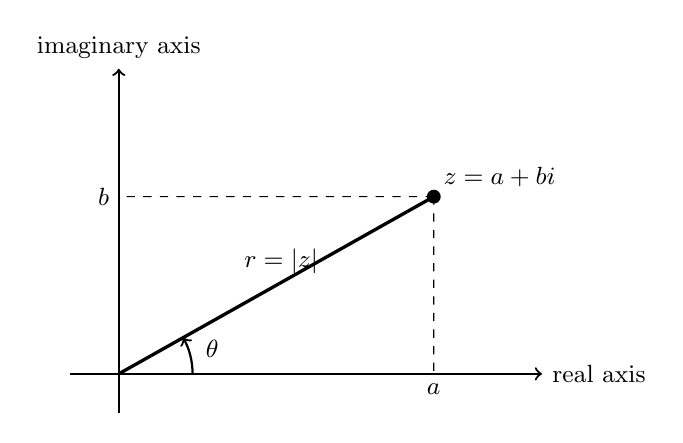
\begin{tikzpicture}[scale=1.25, every node/.style={font=\small}]
  \draw[->, thick] (-0.5,0) -- (4.3,0) node[right] {real axis};
  \draw[->, thick] (0,-0.4) -- (0,3.1) node[above] {imaginary axis};

  \coordinate (Z) at (3.2,1.8);

  \draw[very thick] (0,0) -- (Z);
  \draw[dashed] (Z) -- (3.2,0);
  \draw[dashed] (Z) -- (0,1.8);
  \fill (Z) circle (2pt);

  \node[below] at (3.2,0) {\(a\)};
  \node[left] at (0,1.8) {\(b\)};
  \node[above right] at (Z) {\(z=a+bi\)};

  \draw[->, thick] (0.75,0) arc (0:29.36:0.75);
  \node at (0.95,0.25) {\(\theta\)};
  \node[above] at (1.65,0.92) {\(r=|z|\)};
\end{tikzpicture}
\caption{The complex number \(a+bi\) is the point \((a,b)\) in the plane.}
\label{fig:complex-number-as-point}
\end{figure}

The distance from \(0\) to \(z\) is called the \emph{modulus} of \(z\):

\[
\boxed{
|z|=\sqrt{a^2+b^2}.
}
\]

The angle \(\theta\) that \(z\) makes with the positive real axis is called an
\emph{argument} of \(z\).

Thus

\[
a=r\cos\theta,
\qquad
b=r\sin\theta.
\]

So

\[
z=a+bi
=
r\cos\theta+i r\sin\theta.
\]

Factor out \(r\):

\[
\boxed{
z=r(\cos\theta+i\sin\theta).
}
\]

This is the polar form of a complex number.

\paragraph{Example.}
Write

\[
z=1+i\sqrt3
\]

in polar form.

The modulus is

\[
r=\sqrt{1^2+(\sqrt3)^2}=\sqrt4=2.
\]

The point \((1,\sqrt3)\) lies in Quadrant I, and

\[
\tan\theta=\sqrt3.
\]

Thus

\[
\theta=\frac{\pi}{3}.
\]

So

\[
\boxed{
1+i\sqrt3
=
2\left(\cos\frac{\pi}{3}+i\sin\frac{\pi}{3}\right).
}
\]

As with polar coordinates, the angle is not unique.  We can also write

\[
\theta=\frac{\pi}{3}+2\pi k
\]

for any integer \(k\).

\subsection{Multiplication as scaling and rotation}
\label{subsec:complex-multiplication-scaling-rotation}

The real advantage of polar form appears when we multiply.

Let

\[
z_1=r_1(\cos\alpha+i\sin\alpha)
\]

and

\[
z_2=r_2(\cos\beta+i\sin\beta).
\]

Then

\[
z_1z_2
=
r_1r_2(\cos\alpha+i\sin\alpha)(\cos\beta+i\sin\beta).
\]

Multiply the two parentheses:

\[
(\cos\alpha\cos\beta-\sin\alpha\sin\beta)
+
i(\sin\alpha\cos\beta+\cos\alpha\sin\beta).
\]

By the angle addition formulas,

\[
\cos\alpha\cos\beta-\sin\alpha\sin\beta=\cos(\alpha+\beta),
\]

and

\[
\sin\alpha\cos\beta+\cos\alpha\sin\beta=\sin(\alpha+\beta).
\]

Therefore

\[
\boxed{
z_1z_2
=
r_1r_2\bigl(\cos(\alpha+\beta)+i\sin(\alpha+\beta)\bigr).
}
\]

This is the key rule.

\begin{quote}
\textbf{Multiplication in polar form.}
When complex numbers are multiplied:

\[
\boxed{
\text{moduli multiply}
}
\]

and

\[
\boxed{
\text{arguments add}.
}
\]
\end{quote}

So multiplication by a complex number has two geometric effects:

\[
\text{scale by its modulus}
\]

and

\[
\text{rotate by its argument}.
\]

\paragraph{Example: multiplying by \(i\).}
The number \(i\) has polar form

\[
i=\cos\frac{\pi}{2}+i\sin\frac{\pi}{2}.
\]

Its modulus is \(1\), and its angle is \(\pi/2\).  Therefore multiplying by \(i\) rotates
a point by \(90^\circ\) counterclockwise without changing its distance from the origin.

Algebraically,

\[
i(a+bi)=ai+b i^2=-b+ai.
\]

So multiplication by \(i\) sends

\[
(a,b)
\]

to

\[
(-b,a).
\]

That is exactly a \(90^\circ\) counterclockwise rotation.

\begin{figure}[h]
\centering
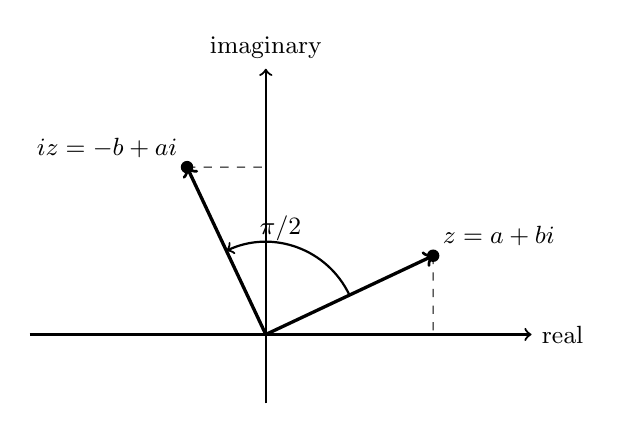
\begin{tikzpicture}[scale=1.25, every node/.style={font=\small}]
  \draw[->, thick] (-2.4,0) -- (2.7,0) node[right] {real};
  \draw[->, thick] (0,-0.7) -- (0,2.7) node[above] {imaginary};

  \coordinate (Z) at (1.7,0.8);
  \coordinate (IZ) at (-0.8,1.7);

  \draw[very thick,->] (0,0) -- (Z);
  \draw[very thick,->] (0,0) -- (IZ);

  \node[anchor=south west] at (Z) {\(z=a+bi\)};
  \node[anchor=south east] at (IZ) {\(iz=-b+ai\)};

  \draw[->, thick] (0.85,0.4) arc (25.2:115.2:0.94);
  \node at (0.15,1.08) {\(\pi/2\)};

  \draw[dashed] (Z) -- (1.7,0);
  \draw[dashed] (IZ) -- (0,1.7);

  \fill (Z) circle (1.8pt);
  \fill (IZ) circle (1.8pt);
\end{tikzpicture}
\caption{Multiplication by \(i\) rotates the plane by \(90^\circ\) counterclockwise.}
\label{fig:multiply-by-i-rotation}
\end{figure}

\paragraph{Example: multiplying two polar numbers.}
Let

\[
z_1=2\left(\cos\frac{\pi}{6}+i\sin\frac{\pi}{6}\right)
\]

and

\[
z_2=3\left(\cos\frac{\pi}{4}+i\sin\frac{\pi}{4}\right).
\]

Then

\[
z_1z_2
=
6\left(\cos\left(\frac{\pi}{6}+\frac{\pi}{4}\right)
+i\sin\left(\frac{\pi}{6}+\frac{\pi}{4}\right)\right).
\]

Since

\[
\frac{\pi}{6}+\frac{\pi}{4}
=
\frac{2\pi}{12}+\frac{3\pi}{12}
=
\frac{5\pi}{12},
\]

we get

\[
\boxed{
z_1z_2
=
6\left(\cos\frac{5\pi}{12}+i\sin\frac{5\pi}{12}\right).
}
\]

The moduli multiplied:

\[
2\cdot3=6.
\]

The angles added:

\[
\frac{\pi}{6}+\frac{\pi}{4}=\frac{5\pi}{12}.
\]

That is the whole multiplication.

\subsection{Euler's formula preview}
\label{subsec:euler-formula-preview}

The expression

\[
\cos\theta+i\sin\theta
\]

appears so often that it deserves a shorter name.

Later, power series will justify the remarkable identity

\[
\boxed{
e^{i\theta}=\cos\theta+i\sin\theta.
}
\]

This is Euler's formula.

For now, read it as a preview and a compact notation for a point on the unit circle.

With Euler's formula, the polar form

\[
z=r(\cos\theta+i\sin\theta)
\]

becomes

\[
\boxed{
z=re^{i\theta}.
}
\]

The multiplication rule becomes almost effortless:

\[
(r_1e^{i\alpha})(r_2e^{i\beta})
=
r_1r_2e^{i(\alpha+\beta)}.
\]

So the usual exponential law

\[
e^Ae^B=e^{A+B}
\]

matches the geometry of rotations.

\begin{quote}
\textbf{Euler's formula as geometry.}
The formula

\[
e^{i\theta}=\cos\theta+i\sin\theta
\]

puts the unit circle into exponential notation.  The angle \(\theta\) becomes the
exponent.
\end{quote}

Some famous special cases fall out immediately.

When

\[
\theta=0,
\]

we get

\[
e^{0}=1.
\]

When

\[
\theta=\frac{\pi}{2},
\]

we get

\[
e^{i\pi/2}=i.
\]

When

\[
\theta=\pi,
\]

we get

\[
e^{i\pi}=-1.
\]

So

\[
\boxed{
e^{i\pi}+1=0.
}
\]

This compact equation connects five fundamental constants:

\[
e,\quad i,\quad \pi,\quad 1,\quad 0.
\]

We will return to the proof after Taylor series, where \(e^x\), \(\sin x\), and \(\cos x\)
will all be written as infinite polynomials.

\subsection{Oscillation written exponentially}
\label{subsec:oscillation-written-exponentially}

Complex numbers also simplify oscillation.

A point moving around the unit circle at angular speed \(\omega\) has complex position

\[
z(t)=e^{i\omega t}.
\]

Using Euler's formula,

\[
z(t)=\cos(\omega t)+i\sin(\omega t).
\]

The real part is

\[
\cos(\omega t),
\]

and the imaginary part is

\[
\sin(\omega t).
\]

So ordinary sine and cosine oscillations are shadows of circular motion.

\begin{figure}[h]
\centering
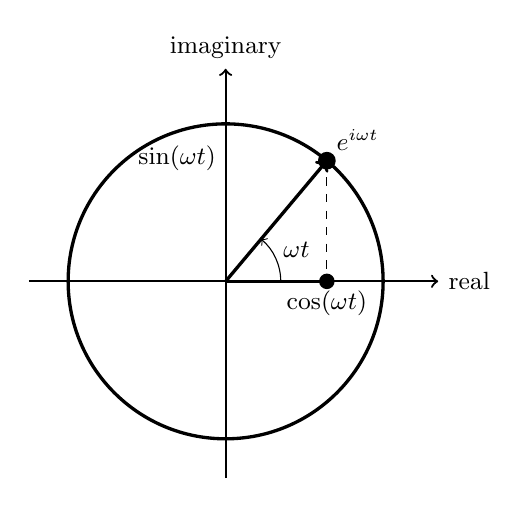
\begin{tikzpicture}[scale=2.0, every node/.style={font=\small}]
  \def\ang{50}
  \coordinate (O) at (0,0);
  \coordinate (P) at ({cos(\ang)},{sin(\ang)});
  \coordinate (X) at ({cos(\ang)},0);

  \draw[->, thick] (-1.25,0) -- (1.35,0) node[right] {real};
  \draw[->, thick] (0,-1.25) -- (0,1.35) node[above] {imaginary};

  \draw[very thick] (O) circle (1);
  \draw[very thick,->] (O) -- (P);
  \draw[dashed] (P) -- (X);
  \draw[very thick] (O) -- (X);

  \fill (P) circle (1.6pt);
  \fill (X) circle (1.4pt);

  \draw[->] (0.35,0) arc (0:\ang:0.35);
  \node at (0.45,0.2) {\(\omega t\)};

  \node[above right] at (P) {\(e^{i\omega t}\)};
  \node[below] at (X) {\(\cos(\omega t)\)};
  \node[left] at (0,0.78) {\(\sin(\omega t)\)};
\end{tikzpicture}
\caption{Sine and cosine are projections of circular motion.  Euler's formula writes that motion as \(e^{i\omega t}\).}
\label{fig:oscillation-complex-exponential}
\end{figure}

The derivative is especially clean.  Starting from

\[
z(t)=\cos(\omega t)+i\sin(\omega t),
\]

differentiate:

\[
z'(t)
=
-\omega\sin(\omega t)+i\omega\cos(\omega t).
\]

Factor out \(i\omega\):

\[
i\omega z(t)
=
i\omega\bigl(\cos(\omega t)+i\sin(\omega t)\bigr).
\]

Since \(i^2=-1\),

\[
i\omega z(t)
=
i\omega\cos(\omega t)-\omega\sin(\omega t).
\]

This matches \(z'(t)\).  Therefore

\[
\boxed{
z'(t)=i\omega z(t).
}
\]

Differentiating again gives

\[
z''(t)=i\omega z'(t)=i\omega(i\omega z(t)).
\]

Since

\[
i^2=-1,
\]

we get

\[
\boxed{
z''(t)=-\omega^2 z(t).
}
\]

Thus

\[
z''+\omega^2z=0.
\]

Taking the real part gives

\[
x(t)=\cos(\omega t),
\]

and

\[
x''+\omega^2x=0.
\]

Taking the imaginary part gives

\[
y(t)=\sin(\omega t),
\]

and again

\[
y''+\omega^2y=0.
\]

\begin{quote}
\textbf{Why complex exponentials are useful.}
The oscillation equation

\[
x''+\omega^2x=0
\]

has sine and cosine solutions.  Complex notation packages both into one function:

\[
e^{i\omega t}.
\]

Differentiation becomes multiplication by \(i\omega\).
\end{quote}

This is a bridge, not a new requirement for the rest of the chapter.  But it shows where
the story is going.

Parametric curves taught us to let time move a point in the plane.  Polar coordinates
taught us to measure that point by radius and angle.  Complex numbers show that the
same plane can be treated as a number system, where multiplication rotates.

The proof of Euler's formula still waits.  To prove it, we need a new kind of infinite
process: not an infinite area, but an infinite sum of functions.
\section{Warning examples}
\label{sec:parametric-polar-warning-examples}

This chapter gave us three new languages for plane curves:

\[
x=x(t),\quad y=y(t),
\]

\[
r=f(\theta),
\]

and

\[
z=re^{i\theta}.
\]

Each language is powerful because it carries more information than a plain Cartesian
equation.  It can tell direction, speed, repeated tracing, and rotation.

That extra information is useful.  It is also dangerous if we forget what the
parameters are doing.

The safest habit is simple:

\[
\boxed{
\text{Before using a formula, ask how the curve is being traced.}
}
\]

\subsection{A parametrization stops even when the curve continues}
\label{subsec:parametrization-stops-curve-continues}

A moving point can pause without the geometric curve having a corner or endpoint.

Consider

\[
x=t^3,
\qquad
y=t^6.
\]

Eliminate the parameter.  Since

\[
x=t^3,
\]

we have

\[
y=t^6=(t^3)^2=x^2.
\]

So the geometric curve is the parabola

\[
y=x^2.
\]

As \(t\) increases through \(0\), the point moves along the parabola through the
origin.

But the velocity is

\[
\frac{dx}{dt}=3t^2,
\qquad
\frac{dy}{dt}=6t^5.
\]

At \(t=0\),

\[
\frac{dx}{dt}=0,
\qquad
\frac{dy}{dt}=0.
\]

The point has zero speed at the origin.

The curve, however, is perfectly smooth there.  The parabola \(y=x^2\) has horizontal
tangent at \((0,0)\).

For \(t\neq0\), the parametric slope is

\[
\frac{dy}{dx}
=
\frac{6t^5}{3t^2}
=
2t^3.
\]

As \(t\to0\),

\[
2t^3\to0.
\]

Thus the tangent slope at the origin is \(0\), even though direct substitution into

\[
\frac{dy/dt}{dx/dt}
\]

would give the meaningless quotient

\[
\frac00.
\]

\begin{figure}[h]
\centering
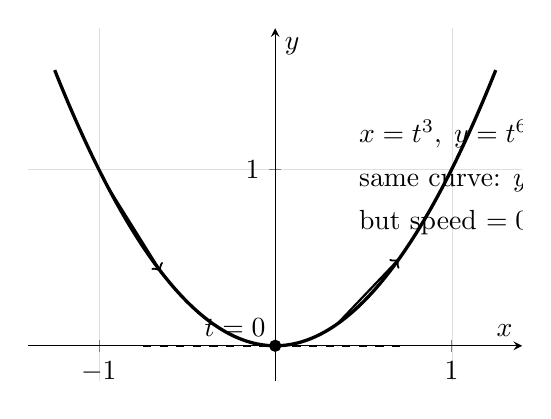
\begin{tikzpicture}
\begin{axis}[
    width=0.70\textwidth,
    height=0.50\textwidth,
    xmin=-1.4, xmax=1.4,
    ymin=-0.2, ymax=1.8,
    axis lines=middle,
    xlabel={\(x\)},
    ylabel={\(y\)},
    xtick={-1,0,1},
    ytick={0,1},
    axis equal image,
    grid=both,
    grid style={line width=.1pt, draw=gray!25},
]
\addplot[very thick, domain=-1.25:1.25, samples=200] {x^2};

% horizontal tangent at origin
\addplot[thick, dashed, domain=-0.75:0.75, samples=2] {0};

% points and arrows along motion
\addplot[only marks, mark=*] coordinates {(0,0)};
\draw[->, thick] (axis cs:-0.95,0.9025) -- (axis cs:-0.65,0.4225);
\draw[->, thick] (axis cs:0.35,0.1225) -- (axis cs:0.70,0.49);

\node[anchor=south east] at (axis cs:0,0) {\(t=0\)};
\node[anchor=west] at (axis cs:0.42,1.2) {\(x=t^3,\;y=t^6\)};
\node[anchor=west] at (axis cs:0.42,0.95) {same curve: \(y=x^2\)};
\node[anchor=west] at (axis cs:0.42,0.70) {but speed \(=0\) at the origin};
\end{axis}
\end{tikzpicture}
\caption{The parametrization \(x=t^3,\;y=t^6\) pauses at the origin, but the geometric curve is the smooth parabola \(y=x^2\).}
\label{fig:parametric-pause-smooth-parabola}
\end{figure}

This is the first warning.

\begin{quote}
\textbf{A zero velocity may be a feature of the parametrization, not a feature of the curve.}

When

\[
x'(t_0)=0
\qquad\text{and}\qquad
y'(t_0)=0,
\]

the moving point stops at \(t=t_0\).  The curve may still be smooth.  The tangent must be
found by looking nearby, not by substituting into the slope quotient.
\end{quote}

A parametrization is a schedule.  A bad or unusual schedule can pause on an otherwise
ordinary road.

\subsection{A polar curve traced twice}
\label{subsec:polar-curve-traced-twice-warning}

Polar coordinates have another kind of trap.  The same point can have many polar
names.

\[
(r,\theta)=(r,\theta+2\pi)=(-r,\theta+\pi).
\]

Because of this, a polar equation may trace a geometric curve more than once.

Consider

\[
r=2\cos\theta.
\]

We converted this earlier:

\[
r^2=2r\cos\theta,
\]

so

\[
x^2+y^2=2x.
\]

Completing the square,

\[
(x-1)^2+y^2=1.
\]

Thus the curve is the circle centered at \((1,0)\) with radius \(1\).

A once-around interval is

\[
-\frac{\pi}{2}\le \theta\le \frac{\pi}{2},
\]

because on that interval

\[
\cos\theta\ge0.
\]

But if we use

\[
0\le\theta\le2\pi,
\]

the circle is traced twice.  The second half is not a new region.  It is the same circle
again, because \(r\) becomes negative and the points are plotted in the opposite
direction.

\begin{figure}[h]
\centering
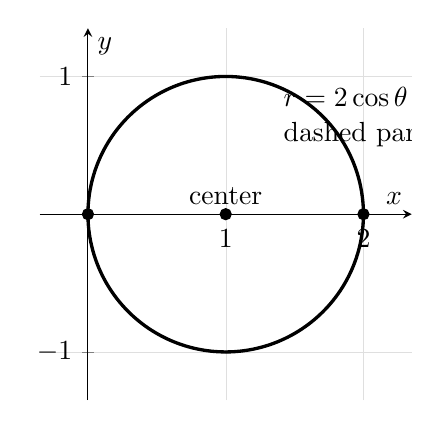
\begin{tikzpicture}
\begin{axis}[
    width=0.68\textwidth,
    height=0.52\textwidth,
    xmin=-0.35, xmax=2.35,
    ymin=-1.35, ymax=1.35,
    axis lines=middle,
    xlabel={\(x\)},
    ylabel={\(y\)},
    xtick={0,1,2},
    ytick={-1,0,1},
    axis equal image,
    grid=both,
    grid style={line width=.1pt, draw=gray!25},
]
% once-around trace
\addplot[very thick, domain=-1.5707963:1.5707963, samples=220]
    ({2*cos(deg(x))*cos(deg(x))},{2*cos(deg(x))*sin(deg(x))});

% retracing interval, drawn dashed on top
\addplot[thick, dashed, domain=1.5707963:4.712389, samples=220]
    ({2*cos(deg(x))*cos(deg(x))},{2*cos(deg(x))*sin(deg(x))});

\addplot[only marks, mark=*] coordinates {(0,0) (2,0) (1,0)};
\node[anchor=south] at (axis cs:1,0) {center};
\node[anchor=west] at (axis cs:1.35,0.85) {\(r=2\cos\theta\)};
\node[anchor=west] at (axis cs:1.35,0.58) {dashed part retraces};
\end{axis}
\end{tikzpicture}
\caption{Using \(0\le\theta\le2\pi\) for \(r=2\cos\theta\) traces the same circle twice.}
\label{fig:polar-circle-traced-twice}
\end{figure}

The area formula reveals the mistake.

If we blindly use \(0\le\theta\le2\pi\), then

\[
A=
\frac12\int_0^{2\pi}(2\cos\theta)^2\,d\theta.
\]

So

\[
A
=
2\int_0^{2\pi}\cos^2\theta\,d\theta
=
2\pi.
\]

But the circle has radius \(1\), so its area is

\[
\pi.
\]

The integral doubled the area because the curve was traced twice.

Use a once-around interval instead:

\[
A=
\frac12\int_{-\pi/2}^{\pi/2}(2\cos\theta)^2\,d\theta.
\]

Then

\[
A=
2\int_{-\pi/2}^{\pi/2}\cos^2\theta\,d\theta
=
2\cdot\frac{\pi}{2}
=
\pi.
\]

\begin{quote}
\textbf{Polar warning.}
The formula

\[
A=\frac12\int_\alpha^\beta r^2\,d\theta
\]

counts how the polar curve is traced on the interval \([\alpha,\beta]\).

If the same region is swept twice, the integral counts it twice.
\end{quote}

The square \(r^2\) makes negative \(r\) look harmless algebraically.  But negative \(r\)
can still change the tracing.

\subsection{A tangent formula fails when both derivatives vanish}
\label{subsec:tangent-formula-fails-both-derivatives-zero}

The parametric slope formula is

\[
\frac{dy}{dx}
=
\frac{dy/dt}{dx/dt}.
\]

It works when

\[
\frac{dx}{dt}\neq0.
\]

For horizontal and vertical tangent tests, we used

\[
\frac{dy}{dt}=0,\quad \frac{dx}{dt}\neq0
\]

and

\[
\frac{dx}{dt}=0,\quad \frac{dy}{dt}\neq0.
\]

Both tests deliberately avoid the case

\[
x'(t)=0
\qquad\text{and}\qquad
y'(t)=0.
\]

Here is why.

At \(t=0\), all three parametrizations below have

\[
x'(0)=0,
\qquad
y'(0)=0.
\]

But their tangent behavior is different.

\[
P_1(t)=(t^2,t^3),
\]

\[
P_2(t)=(t^3,t^2),
\]

\[
P_3(t)=(t^2,t^2).
\]

For \(P_1\),

\[
\frac{dy}{dx}
=
\frac{3t^2}{2t}
=
\frac32t
\qquad (t\neq0).
\]

As \(t\to0\),

\[
\frac32t\to0.
\]

So \(P_1\) has a horizontal tangent at the cusp.

For \(P_2\),

\[
\frac{dy}{dx}
=
\frac{2t}{3t^2}
=
\frac{2}{3t}
\qquad (t\neq0).
\]

As \(t\to0\), this becomes unbounded.  The tangent is vertical.

For \(P_3\),

\[
\frac{dy}{dx}
=
\frac{2t}{2t}
=
1
\qquad (t\neq0).
\]

The curve is the line

\[
y=x
\]

with \(x\ge0\), traced in and out.  Its tangent slope is \(1\).

The same direct substitution,

\[
\frac00,
\]

has hidden three different outcomes.

\begin{figure}[h]
\centering
\begin{minipage}{0.31\textwidth}
\centering
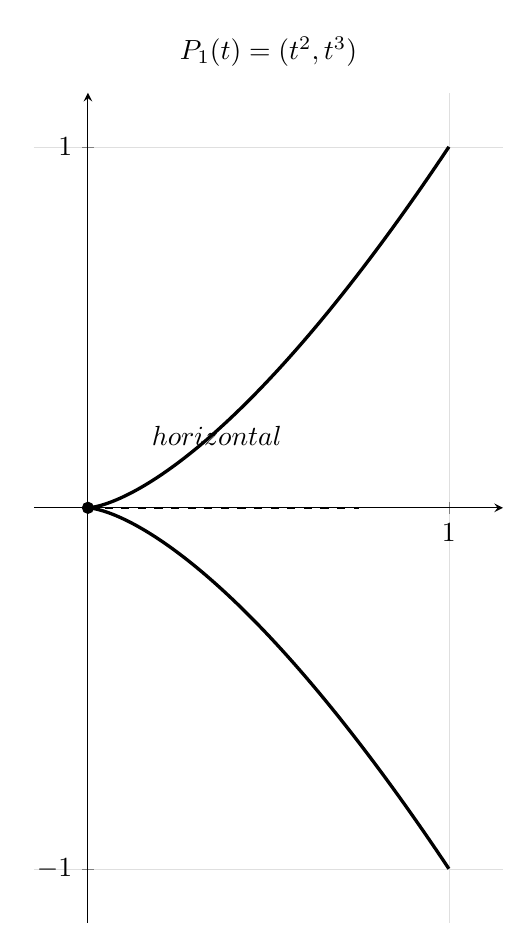
\begin{tikzpicture}
\begin{axis}[
    width=\textwidth,
    height=\textwidth,
    xmin=-0.15, xmax=1.15,
    ymin=-1.15, ymax=1.15,
    axis lines=middle,
    xtick={0,1},
    ytick={-1,0,1},
    axis equal image,
    title={\(P_1(t)=(t^2,t^3)\)},
    grid=both,
    grid style={line width=.1pt, draw=gray!25},
]
\addplot[very thick, domain=-1:1, samples=220] ({x^2},{x^3});
\addplot[thick, dashed, domain=0:0.75, samples=2] {0};
\addplot[only marks, mark=*] coordinates {(0,0)};
\node[anchor=west] at (axis cs:0.15,0.2) {\(\text{horizontal}\)};
\end{axis}
\end{tikzpicture}
\end{minipage}
\hfill
\begin{minipage}{0.31\textwidth}
\centering
\begin{tikzpicture}
\begin{axis}[
    width=\textwidth,
    height=\textwidth,
    xmin=-1.15, xmax=1.15,
    ymin=-0.15, ymax=1.15,
    axis lines=middle,
    xtick={-1,0,1},
    ytick={0,1},
    axis equal image,
    title={\(P_2(t)=(t^3,t^2)\)},
    grid=both,
    grid style={line width=.1pt, draw=gray!25},
]
\addplot[very thick, domain=-1:1, samples=220] ({x^3},{x^2});
\draw[thick, dashed] (axis cs:0,0) -- (axis cs:0,0.8);
\addplot[only marks, mark=*] coordinates {(0,0)};
\node[anchor=west] at (axis cs:0.12,0.55) {\(\text{vertical}\)};
\end{axis}
\end{tikzpicture}
\end{minipage}
\hfill
\begin{minipage}{0.31\textwidth}
\centering
\begin{tikzpicture}
\begin{axis}[
    width=\textwidth,
    height=\textwidth,
    xmin=-0.15, xmax=1.15,
    ymin=-0.15, ymax=1.15,
    axis lines=middle,
    xtick={0,1},
    ytick={0,1},
    axis equal image,
    title={\(P_3(t)=(t^2,t^2)\)},
    grid=both,
    grid style={line width=.1pt, draw=gray!25},
]
\addplot[very thick, domain=-1:1, samples=220] ({x^2},{x^2});
\addplot[thick, dashed, domain=0:0.85, samples=2] {x};
\addplot[only marks, mark=*] coordinates {(0,0)};
\node[anchor=west] at (axis cs:0.15,0.75) {\(\text{slope }1\)};
\end{axis}
\end{tikzpicture}
\end{minipage}
\caption{At \(t=0\), all three parametrizations have \(x'(0)=y'(0)=0\), but their tangents are different.}
\label{fig:three-zero-velocity-tangent-outcomes}
\end{figure}

\begin{quote}
\textbf{The \(0/0\) tangent warning.}
When both coordinate derivatives vanish, the slope formula does not decide the
tangent.

Look at the nearby slopes, eliminate the parameter if possible, or study the local
geometry.
\end{quote}

The same warning applies to polar curves.  For

\[
x=r(\theta)\cos\theta,
\qquad
y=r(\theta)\sin\theta,
\]

if

\[
\frac{dx}{d\theta}=0
\qquad\text{and}\qquad
\frac{dy}{d\theta}=0,
\]

then the polar slope formula gives \(0/0\).  A cusp, a smooth pause, a retracing, or a
more complicated behavior may be hiding there.

\subsection{The chapter's main cautions}
\label{subsec:chapter-main-cautions}

The formulas in this chapter are reliable when their hypotheses match the tracing.

\begin{center}
\begin{tabular}{c|p{0.62\textwidth}}
\textbf{situation} & \textbf{what to check} \\ \hline
Parametric slope & Is \(dx/dt\neq0\)? If both \(dx/dt\) and \(dy/dt\) vanish, study nearby motion. \\[3pt]
Parametric length & Does the parametrization retrace the curve? The length integral counts distance traveled. \\[3pt]
Parametric area & Is the curve traced once? What is the orientation? \\[3pt]
Polar area & What interval of \(\theta\) sweeps the region exactly once? Does \(r\) become negative? \\[3pt]
Polar intersections & Did the curves meet at the origin or with different polar names? \\[3pt]
Conic classification & First rewrite the denominator so the constant term is \(1\), then read eccentricity. \\[3pt]
Complex polar form & Remember that arguments are not unique: \(\theta\) and \(\theta+2\pi k\) describe the same direction.
\end{tabular}
\end{center}

A formula is a tool, not a substitute for the picture.

\section{Chapter review and projects}
\label{sec:chapter-review-parametric-polar-conics}

This chapter began with a simple move: instead of forcing a curve to be a graph
\(y=f(x)\), let a moving point draw it.

That one move opened many doors.

A circle could be traced by

\[
x=\cos t,
\qquad
y=\sin t.
\]

A rolling wheel produced a cycloid.

A rotating ray produced polar coordinates.

A focus and directrix produced conics.

A point \(x+iy\) became a complex number, and multiplication became scaling plus
rotation.

The theme stayed the same:

\[
\boxed{
\text{Choose coordinates that match the geometry.}
}
\]

\subsection{Chapter map}
\label{subsec:chapter-map-parametric-polar}

\begin{center}
\begin{tabular}{c|p{0.58\textwidth}}
\textbf{language} & \textbf{best suited for} \\ \hline
Cartesian \(y=f(x)\) & Graphs that pass the vertical line test; ordinary derivative and integral formulas. \\[3pt]
Parametric \(x=x(t),\;y=y(t)\) & Curves traced by motion, loops, cusps, rolling curves, and curves not expressible as one graph. \\[3pt]
Polar \(r=f(\theta)\) & Rotation, spirals, radial distance, roses, limacons, and conics with a focus at the pole. \\[3pt]
Complex \(z=re^{i\theta}\) & Scaling, rotation, circular motion, oscillation, and the preview of Euler's formula.
\end{tabular}
\end{center}

No coordinate system is universally best.  The skill is knowing which one makes the
structure visible.

\subsection{Essential formulas}
\label{subsec:essential-formulas-parametric-polar}

\subsubsection*{Parametric curves}

For

\[
x=x(t),
\qquad
y=y(t),
\]

the velocity components are

\[
x'(t),
\qquad
y'(t).
\]

The speed is

\[
\boxed{
\sqrt{(x'(t))^2+(y'(t))^2}.
}
\]

The slope is

\[
\boxed{
\frac{dy}{dx}
=
\frac{dy/dt}{dx/dt}
}
\]

when \(dx/dt\neq0\).

The second derivative is

\[
\boxed{
\frac{d^2y}{dx^2}
=
\frac{\dfrac{d}{dt}\left(\dfrac{dy}{dx}\right)}{dx/dt}.
}
\]

The length from \(t=a\) to \(t=b\) is

\[
\boxed{
L=
\int_a^b
\sqrt{(x'(t))^2+(y'(t))^2}\,dt.
}
\]

If a simple closed curve is traced once counterclockwise, its area is

\[
\boxed{
A=
\frac12\int_a^b
\left(x(t)y'(t)-y(t)x'(t)\right)\,dt.
}
\]

\subsubsection*{Polar coordinates}

The conversion formulas are

\[
\boxed{
x=r\cos\theta,
\qquad
y=r\sin\theta,
\qquad
r^2=x^2+y^2.
}
\]

For a polar curve

\[
r=r(\theta),
\]

we can view it as the parametric curve

\[
x=r(\theta)\cos\theta,
\qquad
y=r(\theta)\sin\theta.
\]

The slope is

\[
\boxed{
\frac{dy}{dx}
=
\frac{r'(\theta)\sin\theta+r(\theta)\cos\theta}
{r'(\theta)\cos\theta-r(\theta)\sin\theta}.
}
\]

The polar area formula is

\[
\boxed{
A=\frac12\int_\alpha^\beta r(\theta)^2\,d\theta.
}
\]

The polar length formula is

\[
\boxed{
L=
\int_\alpha^\beta
\sqrt{r(\theta)^2+\bigl(r'(\theta)\bigr)^2}\,d\theta.
}
\]

\subsubsection*{Conics}

The focus-directrix definition is

\[
\boxed{
\operatorname{dist}(P,F)=e\,\operatorname{dist}(P,\ell).
}
\]

The eccentricity \(e\) determines the conic:

\begin{center}
\begin{tabular}{c|c}
\textbf{eccentricity} & \textbf{conic} \\ \hline
\(0<e<1\) & ellipse \\[3pt]
\(e=1\) & parabola \\[3pt]
\(e>1\) & hyperbola
\end{tabular}
\end{center}

With the focus at the pole, common polar conic forms are

\[
\boxed{
r=\frac{p}{1\pm e\cos\theta}
}
\]

and

\[
\boxed{
r=\frac{p}{1\pm e\sin\theta}.
}
\]

For an ellipse with semi-major axis \(a\) and eccentricity \(e\),

\[
\boxed{
p=a(1-e^2).
}
\]

\subsubsection*{Complex polar form}

A complex number

\[
z=a+bi
\]

has modulus

\[
|z|=\sqrt{a^2+b^2}.
\]

In polar form,

\[
\boxed{
z=r(\cos\theta+i\sin\theta).
}
\]

Euler's formula, to be justified later by power series, is

\[
\boxed{
e^{i\theta}=\cos\theta+i\sin\theta.
}
\]

So the compact polar form is

\[
\boxed{
z=re^{i\theta}.
}
\]

Multiplication becomes

\[
\boxed{
(r_1e^{i\alpha})(r_2e^{i\beta})
=
r_1r_2e^{i(\alpha+\beta)}.
}
\]

In words:

\[
\boxed{
\text{multiply moduli and add arguments.}
}
\]

\subsection{Skills: parametric and polar calculus}
\label{subsec:skills-parametric-polar-calculus}

By the end of this chapter, the reader should be able to do the following.

\begin{enumerate}
\item Sketch a parametric curve by plotting key parameter values and indicating direction.

\item Eliminate a parameter when possible, while keeping the parameter interval in mind.

\item Distinguish between a geometric curve and a parametrized motion along the curve.

\item Find

\[
\frac{dy}{dx}
\]

for a parametric curve and use it to find tangent lines.

\item Identify horizontal and vertical tangents for parametric and polar curves.

\item Compute parametric arc length as accumulated speed.

\item Compute the area enclosed by a simple closed parametric curve, including the sign
from orientation.

\item Convert between Cartesian and polar coordinates.

\item Sketch basic polar curves: circles, spirals, roses, limacons, and cardioids.

\item Use

\[
A=\frac12\int r^2\,d\theta
\]

to compute polar areas, after choosing an interval that traces the region once.

\item Use

\[
L=\int \sqrt{r^2+(r')^2}\,d\theta
\]

to compute polar arc length.

\item Recognize when a polar curve is retraced or when negative \(r\) creates an inner loop.

\item Classify conics from eccentricity and convert simple conics between standard and polar form.

\item Interpret complex multiplication as scaling and rotation.

\item Recognize \(e^{i\theta}\) as the notation that packages circular motion.
\end{enumerate}

\subsection{Review problems}
\label{subsec:chapter-14-review-problems}

\begin{enumerate}
\item The curve

\[
x=1+2t,
\qquad
y=3-t,
\qquad
0\le t\le2
\]

is a line segment.  Find its endpoints, direction of travel, Cartesian equation, and length.

\item For

\[
x=t^2-4,
\qquad
y=t^3-3t,
\]

find

\[
\frac{dy}{dx}
\]

and determine where the curve has horizontal or vertical tangents.

\item For

\[
x=\cos t+\sin t,
\qquad
y=\sin t-\cos t,
\qquad
0\le t\le2\pi,
\]

show that the curve is a circle.  Determine its center, radius, and speed.

\item Find the length of one arch of the cycloid

\[
x=R(t-\sin t),
\qquad
y=R(1-\cos t),
\qquad
0\le t\le2\pi.
\]

Then explain why the endpoints are cusps.

\item A simple closed curve is traced by

\[
x=2\cos t,
\qquad
y=3\sin t,
\qquad
0\le t\le2\pi.
\]

Use the parametric area formula to find the enclosed area.

\item Convert the polar point

\[
\left(-3,\frac{\pi}{6}\right)
\]

to Cartesian coordinates.  Then give two other polar names for the same point.

\item Convert the polar equation

\[
r=4\sin\theta
\]

to Cartesian form and identify the curve.

\item Find the slope of the polar curve

\[
r=1+\cos\theta
\]

at

\[
\theta=\frac{\pi}{2}.
\]

\item Find the area enclosed by the cardioid

\[
r=2+2\cos\theta.
\]

\item Find the area of one petal of

\[
r=3\sin(2\theta).
\]

Be careful to choose an interval that traces one petal exactly once.

\item Classify the conic

\[
r=\frac{8}{4-3\cos\theta}.
\]

Then identify its eccentricity.

\item Convert

\[
r=\frac{6}{1+\cos\theta}
\]

to Cartesian form and identify the conic.

\item Write

\[
z=-1+i\sqrt3
\]

in polar form.

\item Use polar form to compute

\[
\left(2e^{i\pi/6}\right)\left(5e^{i2\pi/3}\right).
\]

Then describe the multiplication geometrically.

\item For each expression, decide whether it is mainly a Cartesian, parametric, polar, or
complex description.

\[
y=x^2,
\qquad
x=t-\sin t,\;y=1-\cos t,
\qquad
r=1+\cos\theta,
\qquad
z=3e^{i\theta}.
\]

Explain what feature of the curve or motion each description makes easiest to see.
\end{enumerate}

\subsection{Project: design a cycloid animation}
\label{subsec:project-cycloid-animation}

A cycloid is not just a curve.  It is a record of rolling motion.  This project asks for an
animation or a sequence of frames showing how the curve is created.

Use radius

\[
R=1
\]

unless there is a reason to choose another value.

The center of the rolling circle is

\[
C(t)=(t,1).
\]

The point on the rim is

\[
P(t)=(t-\sin t,\,1-\cos t).
\]

The cycloid is the path of \(P(t)\) for

\[
0\le t\le2\pi.
\]

\paragraph{Tasks.}

\begin{enumerate}
\item Draw the wheel at several values of \(t\), such as

\[
0,\quad \frac{\pi}{4},\quad \frac{\pi}{2},\quad \pi,\quad \frac{3\pi}{2},\quad 2\pi.
\]

For each frame, show the center \(C(t)\), the rolling circle, the point \(P(t)\), and the
portion of the cycloid already traced.

\item Verify algebraically that \(P(t)\) lies on the wheel by showing

\[
\operatorname{dist}(P(t),C(t))=1.
\]

\item Explain why the center has moved distance \(t\) when the wheel has rotated through
angle \(t\).  This is the no-slipping condition.

\item Differentiate \(P(t)\) and compute the speed:

\[
\sqrt{(x'(t))^2+(y'(t))^2}.
\]

Show that on \(0\le t\le2\pi\),

\[
\text{speed}=2\sin\left(\frac t2\right).
\]

\item Use numerical integration to estimate the length of one arch.  Compare your estimate
with the exact value

\[
8.
\]

\item Use numerical integration to estimate the area under one arch.  Compare your
estimate with the exact value

\[
3\pi.
\]
\end{enumerate}

\paragraph{Deliverable.}
The final result should include the animation or frame sequence, the formulas used to
generate it, and a short explanation of why the cusps occur at the beginning and end of
the arch.

\begin{figure}[h]
\centering
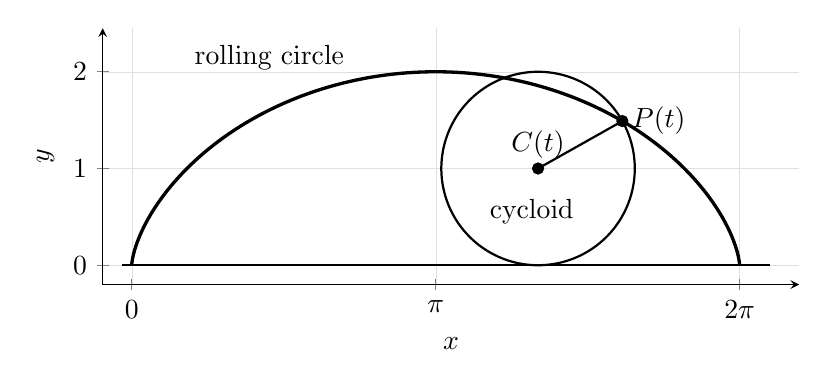
\begin{tikzpicture}
\begin{axis}[
    width=0.86\textwidth,
    height=0.42\textwidth,
    xmin=-0.3, xmax=6.9,
    ymin=-0.2, ymax=2.45,
    axis lines=left,
    xlabel={\(x\)},
    ylabel={\(y\)},
    xtick={0,3.14159,6.28318},
    xticklabels={\(0\),\(\pi\),\(2\pi\)},
    ytick={0,1,2},
    axis equal image,
    grid=both,
    grid style={line width=.1pt, draw=gray!25},
]
% cycloid
\addplot[very thick, domain=0:6.283185, samples=280]
    ({x - sin(deg(x))},{1 - cos(deg(x))});

% wheel at t = 4.2
\def\tval{4.2}
\addplot[thick, domain=0:360, samples=160]
    ({\tval + cos(x)},{1 + sin(x)});

% center and point
\addplot[only marks, mark=*] coordinates {(\tval,1)};
\addplot[only marks, mark=*] coordinates
    {({\tval - sin(deg(\tval))},{1 - cos(deg(\tval))})};

% radius line
\draw[thick] (axis cs:\tval,1) --
    (axis cs:{\tval - sin(deg(\tval))},{1 - cos(deg(\tval))});

% ground
\addplot[thick, domain=-0.1:6.6, samples=2] {0};

\node[anchor=south] at (axis cs:\tval,1) {\(C(t)\)};
\node[anchor=west] at (axis cs:{\tval - sin(deg(\tval))},{1 - cos(deg(\tval))}) {\(P(t)\)};
\node[anchor=west] at (axis cs:0.55,2.15) {rolling circle};
\node[anchor=west] at (axis cs:3.6,0.55) {cycloid};
\end{axis}
\end{tikzpicture}
\caption{A cycloid animation should show the rolling circle and the point \(P(t)\) tracing the curve.}
\label{fig:cycloid-animation-project}
\end{figure}

\subsection{Project: compare polar and Cartesian descriptions of conics}
\label{subsec:project-compare-polar-cartesian-conics}

Conics have two personalities.

A Cartesian equation often makes the center, axes, vertices, and asymptotes visible.

A polar equation often makes the focus, directrix, eccentricity, and orbital meaning
visible.

This project compares those two descriptions.

Start with the polar family

\[
r=\frac{p}{1+e\cos\theta},
\qquad p>0.
\]

The focus is at the pole.

\paragraph{Tasks.}

\begin{enumerate}
\item Choose one value of \(p\), such as

\[
p=2.
\]

Then graph three curves using

\[
e=\frac12,
\qquad
e=1,
\qquad
e=\frac32.
\]

Classify them as ellipse, parabola, or hyperbola.

\item Convert the polar equation to Cartesian form.

Begin with

\[
r(1+e\cos\theta)=p.
\]

Use

\[
r\cos\theta=x
\]

to get

\[
r+ex=p.
\]

Then write

\[
r=\sqrt{x^2+y^2}
\]

and square carefully.

\item Show that the Cartesian equation becomes

\[
(1-e^2)x^2+y^2+2pex-p^2=0.
\]

\item For

\[
0<e<1,
\]

complete the square and write the equation in ellipse form.  Identify the center, the
semi-major axis \(a\), and the eccentricity.

\item For

\[
e=1,
\]

show that the equation reduces to a parabola.  Identify its vertex and direction of
opening.

\item For

\[
e>1,
\]

complete the square and write the equation in hyperbola form.  Identify the center,
vertices, and asymptotes.

\item Write a short comparison answering these questions:

Which form makes eccentricity easiest to read?

Which form makes the center easiest to read?

Which form makes the focus easiest to locate?

Which form is better for describing planetary motion?

Which form is better for graphing with rectangular axes?
\end{enumerate}

\paragraph{Deliverable.}
The final project should include at least three graphs, the algebraic conversion, and a
short written comparison of the two coordinate systems.

\subsection{The bridge to infinite series}
\label{subsec:hook-to-infinite-series}

The chapter ends with a preview that has not yet been proved:

\[
e^{i\theta}=\cos\theta+i\sin\theta.
\]

This formula says that an exponential can move around a circle.

But why should an exponential know anything about sine and cosine?

The proof comes from a new kind of infinite process.  Not an infinite subdivision of an
area.  Not an infinite limiting process of slopes.  This time the infinite process is an
infinite sum:

\[
1+x+\frac{x^2}{2!}+\frac{x^3}{3!}+\cdots.
\]

The next chapter begins there.

\[
\boxed{
\text{Calculus now turns from curves and coordinates to sequences and infinite series.}
}
\]
